\documentclass{beamer}

\usetheme{default}
\usecolortheme{default}
\usefonttheme[onlymath]{serif}

%%%%% PACKAGES

% small tweaks and nicer typography
\usepackage{microtype}

% changes language to German
% gives proper date, and correct hyphenation
\usepackage[ngerman]{babel}
\uselanguage{German}
\languagepath{German}

% display quotes correctly
\usepackage{csquotes}

% basic math stuff
\usepackage{mathtools}
\usepackage{amssymb}
\usepackage{amsthm}
\usepackage{tikz}

% allow for any font-size, alternative mathpazo
\usepackage{mathptmx}

% images
\usepackage{graphicx}
\graphicspath{ {./Plots} }
\usepackage{subcaption}

% tikz
\usepackage{tikz}
\usetikzlibrary{positioning}
\usetikzlibrary{babel}
\tikzset{>=stealth}

\newcommand{\tikzmark}[3][]{\tikz[remember picture,baseline] \node [anchor=base,#1](#2) {$#3$};}

% Tikz librarys
\usetikzlibrary{datavisualization}
\usetikzlibrary{datavisualization.formats.functions}
%\usetikzlibrary{external}
%\tikzexternalize[prefix=../Resources/]


%%%%% CONFIGURATION

% prevents automatic line breaks inside of equations
% since it looks bad
\binoppenalty = \maxdimen
\relpenalty   = \maxdimen

% theorem-like environments
\newcounter{everything}
%\newtheorem{corollary}[everything]{Korollar}
%\newtheorem{lemma}[everything]{Lemma}
\newtheorem{proposition}[everything]{Proposition}



%%%%% CUSTOM COMMANDS


% real numbers via \R
% complex numbers via \C
% general field via \K
\def\C{\mathbb{C}}
\def\R{\mathbb{R}}
\def\K{\mathbb{K}}
\def\Q{\mathbb{Q}}
\def\Z{\mathbb{Z}}
\def\N{\mathbb{N}}
\def\H{\mathbb{H}}
\def\e{\varepsilon}
\def\ev{e}


\newcommand{\cA}{\mathcal{A}}
\newcommand{\cB}{\mathcal{B}}
\newcommand{\cC}{\mathcal{C}}
\newcommand{\cD}{\mathcal{D}}
\newcommand{\cE}{\mathcal{E}}
\newcommand{\cF}{\mathcal{F}}
\newcommand{\cG}{\mathcal{G}}
\newcommand{\cH}{\mathcal{H}}
\newcommand{\cI}{\mathcal{I}}
\newcommand{\cJ}{\mathcal{J}}
\newcommand{\cK}{\mathcal{K}}
\newcommand{\cL}{\mathcal{L}}
\newcommand{\cM}{\mathcal{M}}
\newcommand{\cN}{\mathcal{N}}
\newcommand{\cO}{\mathcal{O}}
\newcommand{\cP}{\mathcal{P}}
\newcommand{\cQ}{\mathcal{Q}}
\newcommand{\cR}{\mathcal{R}}
\newcommand{\cS}{\mathcal{S}}
\newcommand{\cT}{\mathcal{T}}
\newcommand{\cU}{\mathcal{U}}
\newcommand{\cV}{\mathcal{V}}
\newcommand{\cW}{\mathcal{W}}
\newcommand{\cX}{\mathcal{X}}
\newcommand{\cY}{\mathcal{Y}}
\newcommand{\cZ}{\mathcal{Z}}

\newcommand{\bA}{\mathbb{A}}
\newcommand{\bB}{\mathbb{B}}
\newcommand{\bC}{\mathbb{C}}
\newcommand{\bD}{\mathbb{D}}
\newcommand{\bE}{\mathbb{E}}
\newcommand{\bF}{\mathbb{F}}
\newcommand{\bG}{\mathbb{G}}
\newcommand{\bH}{\mathbb{H}}
\newcommand{\bI}{\mathbb{I}}
\newcommand{\bJ}{\mathbb{J}}
\newcommand{\bK}{\mathbb{K}}
\newcommand{\bL}{\mathbb{L}}
\newcommand{\bM}{\mathbb{M}}
\newcommand{\bN}{\mathbb{N}}
\newcommand{\bO}{\mathbb{O}}
\newcommand{\bP}{\mathbb{P}}
\newcommand{\bQ}{\mathbb{Q}}
\newcommand{\bR}{\mathbb{R}}
\newcommand{\bS}{\mathbb{S}}
\newcommand{\bT}{\mathbb{T}}
\newcommand{\bU}{\mathbb{U}}
\newcommand{\bV}{\mathbb{V}}
\newcommand{\bW}{\mathbb{W}}
\newcommand{\bX}{\mathbb{X}}
\newcommand{\bY}{\mathbb{Y}}
\newcommand{\bZ}{\mathbb{Z}}

\newcommand{\hu}{\hat{u}}
\newcommand{\hv}{\hat{v}}
\newcommand{\hV}{\hat{V}}
\newcommand{\hw}{\hat{w}}
\newcommand{\hW}{\hat{W}}
\newcommand{\hA}{\hat{A}}
\newcommand{\hC}{\hat{C}}
\newcommand{\hR}{\hat{R}}
\newcommand{\hQ}{\hat{Q}}
\newcommand{\hq}{\hat{q}}
\newcommand{\hp}{\hat{p}}
\newcommand{\hl}{\hat{\ell}}
\newcommand{\hlambda}{\hat{\lambda}}
\newcommand{\ha}{\hat{a}}
\newcommand{\hb}{\hat{b}}


\newcommand{\tiS}{\tilde{S}}
\newcommand{\tiu}{\tilde{u}}
\newcommand{\tih}{\tilde{h}}
\newcommand{\tie}{\tilde{\e}}
\newcommand{\tisigma}{\tilde{\sigma}}


%%%%%%%%%%%%%%%%%%% Math operators %%%%%%%%%%%%%


\newcommand{\dif}[1]{\,\mathrm{d} #1}
\newcommand{\norm}[1]{\lVert #1 \rVert}
\newcommand{\bnorm}[1]{\left\lVert #1\right\rVert}
\newcommand{\vii}[2]{\ensuremath{\begin{pmatrix}#1 \\ #2 \end{pmatrix}}}
\newcommand{\mii}[4]{\ensuremath{\begin{pmatrix}#1&#2 \\ #3&#4 \end{pmatrix}}}
\newcommand{\mc}[1]{\mathcal{#1}}


% Hom(V,W) via \Hom(V,W)
\DeclareMathOperator{\End}{End}
\DeclareMathOperator{\Hom}{Hom}
\DeclareMathOperator{\Id}{Id}
\DeclareMathOperator{\diver}{Div}
\DeclareMathOperator{\Tr}{Tr}
\DeclareMathOperator{\Image}{Image}
\DeclareMathOperator{\Span}{Span}         % linear span
\DeclareMathOperator{\Vspan}{Span}
\DeclareMathOperator{\Erf}{erf}
\DeclareMathOperator{\epi}{epi}

% inner product (scalar product) via \inner{v, w}
% norm via \norm{x}
% absolute value via \abs{x}
% use the star-version for automatic scaling
\DeclarePairedDelimiter{\abs}{|}{|}
\DeclarePairedDelimiter{\inner}{\langle}{\rangle}

% \vect{ x // y // z } for a column vector with entries x, y, z
% similarly for larger vectors
% in this code:  1 = number of arguments
%               #1 = first argument
\newcommand{\vect}[1]{\begin{bmatrix} #1 \end{bmatrix}}
\newcommand{\conj}{\overline}


% \conj{z} for complex conjugation
% \newcommand{\conj}{\overline}

%%%%% allow for proofs over multiple slides

\makeatletter
\newenvironment<>{proofs}[1][\proofname]{%
    \par
    \def\insertproofname{#1\@addpunct{.}}%
    \usebeamertemplate{proof begin}#2}
  {\usebeamertemplate{proof end}}
\makeatother


%%%%% TITLE PAGE

\subject{Adaptive Finite Elemente für Lineare Elastizität}
\title{Adaptive Finite Elemente für Lineare Elastizität}
%\subtitle{Blatt 0}
\author{Theo Koppenhöfer}
\date{25. Mai 2022}




\begin{document}

\frame[plain]



% Frame 1
\frame[plain]{\titlepage}

\begin{frame}
	\begin{center}
		\Large{{Es wird spannender...}}
	\end{center}
\end{frame}

% Frame 3
\frame{ \frametitle{Outline} \tableofcontents }

\section{Einführendes Beispiel}
\begin{frame}
	\frametitle{Ein einführendes Beispiel}
	\begin{figure}[h]
	    \centering
	    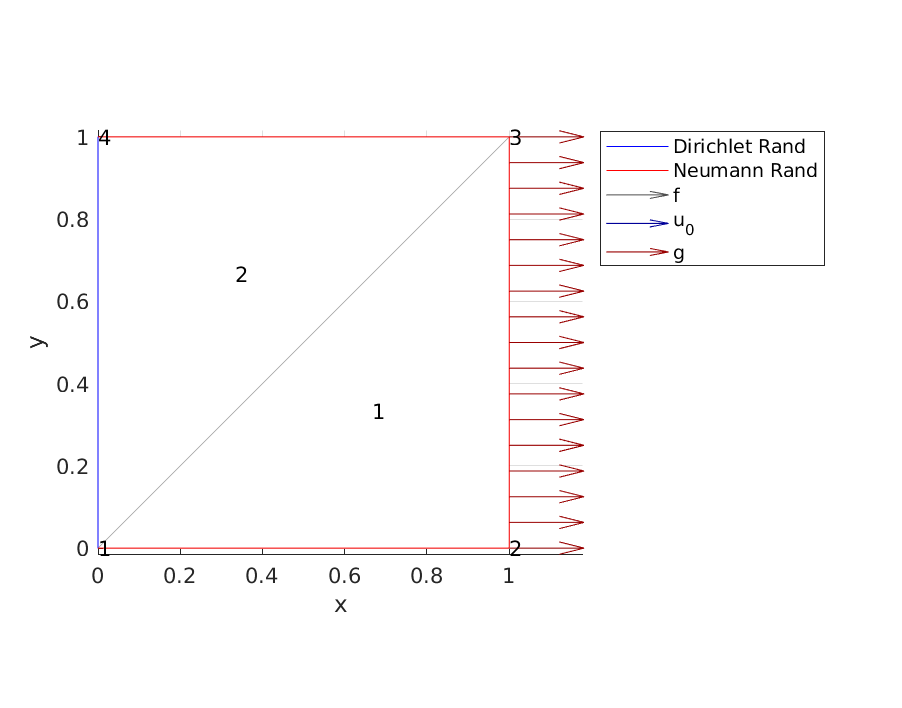
\includegraphics[width=\textwidth]{./Plots/PullBoxInitial1}
	    \caption{Anfangskonfiguration}
	\end{figure}
\end{frame}

\begin{frame}
	\begin{figure}[h]
	    \centering
	    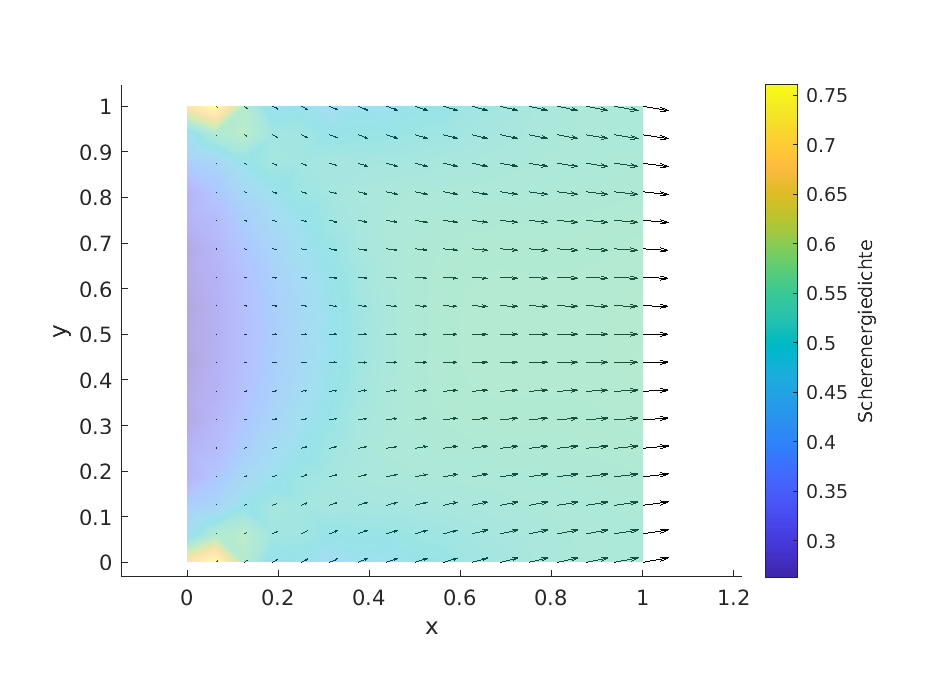
\includegraphics[width=\textwidth]{./Plots/PullBoxSoln1}
	    \caption{Numerische Lösung auf dem Gebiet}
	\end{figure}
\end{frame}

\begin{frame}
	\begin{figure}[h]
	    \centering
	    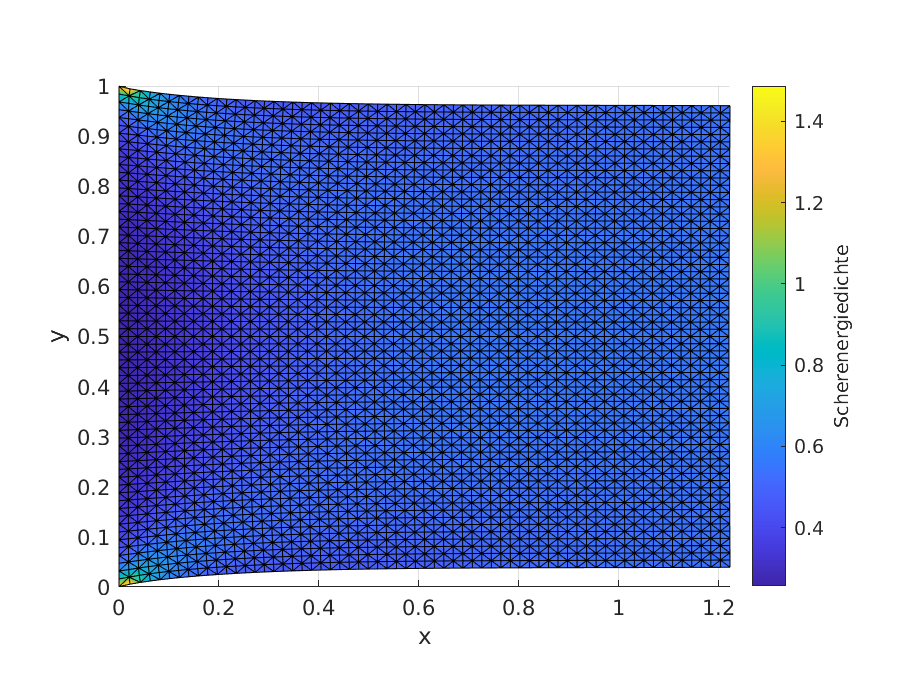
\includegraphics[width=\textwidth]{./Plots/PullBoxUniformSoln1}
	    \caption{Lösung mit uniformer Triangulierung}
	\end{figure}
\end{frame}

\begin{frame}
	Fragen, die man sich stellen kann
	\begin{itemize}
		\item 
		Wie kann ich den Fehler der berechneten Lösung abschätzen, ohne die genaue Lösung zu kennen? $\rightarrow$ Fehlerschätzer
		\item
		Wie kann ich das die Kenntnis über diesen Fehler gewinnbringend verwenden? $\rightarrow$ adaptive Gitterverfeinerung
	\end{itemize}
\end{frame}

\begin{frame}
	\begin{figure}[h]
	    \centering
	    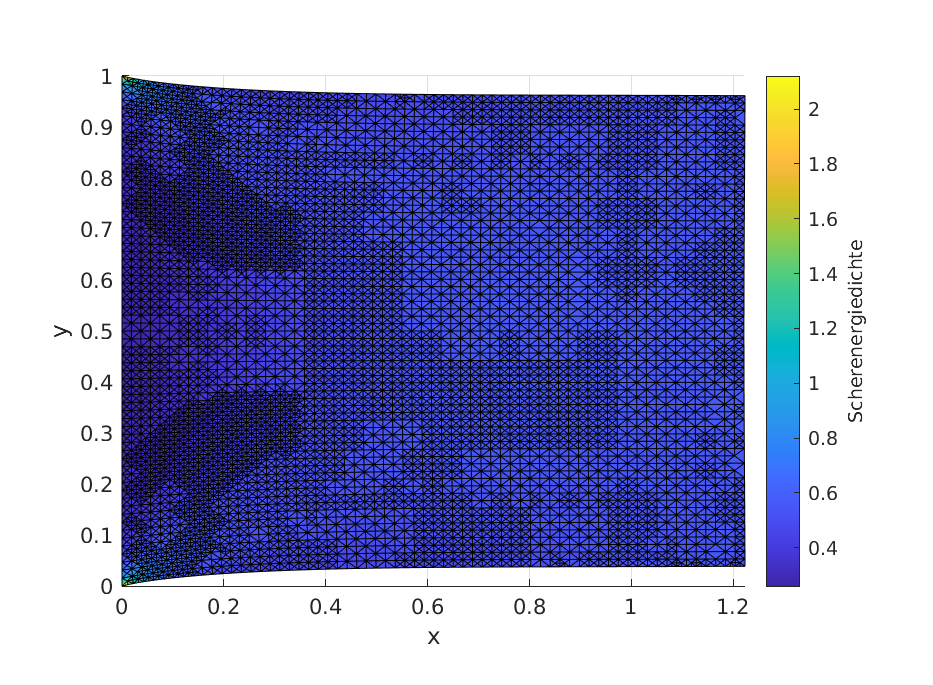
\includegraphics[width=\textwidth]{./Plots/PullBoxAdaptiveSoln1}
	    \caption{Lösung mit adaptiven Methoden}
	\end{figure}
\end{frame}


\section{Formulierungen des kontinuierlichen Problems}
\subsection*{Erste Formulierung}
\subsubsection*{Geometrische Betrachtungen}
\begin{frame}
	\frametitle{Formulierung des Problems}
	Wir nehmen an, der Körper nimmt in Referenzkonfiguration (Lagrange-Koordinaten) das Gebiet $\overline{\Omega}\subseteq\R^d$ ein. Wir bezeichnen
	\begin{itemize}
		\item Deformation: Eine Abbildung $\chi\colon\overline{\Omega}\to\R^d$ mit $\det\nabla\chi>0$
		\item Verschiebung: Eine Abbildung $u$, gegeben durch $\chi=\Id+u$
	\end{itemize}
	Die Menge an zulässigen Verschiebungen bezeichnen wir mit $V$ (wir verwenden für eine generische Verschiebung den Buchstaben $v$).
\end{frame}
\begin{frame}
	\begin{figure}[h]
	\centering
	% Graphic for TeX using PGF
% Title: /mnt/12CCB7B3CCB79009/Filing/Education/University/Bonn/Courses/Bachelorarbeit/Resources/Deformation1.dia
% Creator: Dia v0.97+git
% CreationDate: Mon Apr  4 15:27:10 2022
% For: theo
% \usepackage{tikz}
% The following commands are not supported in PSTricks at present
% We define them conditionally, so when they are implemented,
% this pgf file will use them.
\ifx\du\undefined
  \newlength{\du}
\fi
\setlength{\du}{15\unitlength}
\begin{tikzpicture}[even odd rule]
\pgftransformxscale{0.5}
\pgftransformyscale{-0.5}
\definecolor{dialinecolor}{rgb}{0.000000, 0.000000, 0.000000}
\pgfsetstrokecolor{dialinecolor}
\pgfsetstrokeopacity{1.000000}
\definecolor{diafillcolor}{rgb}{1.000000, 1.000000, 1.000000}
\pgfsetfillcolor{diafillcolor}
\pgfsetfillopacity{1.000000}
\pgfsetlinewidth{0.100000\du}
\pgfsetdash{}{0pt}
\pgfsetbuttcap
{
\definecolor{diafillcolor}{rgb}{0.000000, 0.000000, 0.000000}
\pgfsetfillcolor{diafillcolor}
\pgfsetfillopacity{1.000000}
% was here!!!
\pgfsetarrowsend{latex}
\definecolor{dialinecolor}{rgb}{0.000000, 0.000000, 0.000000}
\pgfsetstrokecolor{dialinecolor}
\pgfsetstrokeopacity{1.000000}
\draw (0.000000\du,0.000000\du)--(5.000000\du,0.000000\du);
}
\pgfsetlinewidth{0.100000\du}
\pgfsetdash{}{0pt}
\pgfsetbuttcap
{
\definecolor{diafillcolor}{rgb}{0.000000, 0.000000, 0.000000}
\pgfsetfillcolor{diafillcolor}
\pgfsetfillopacity{1.000000}
% was here!!!
\pgfsetarrowsend{latex}
\definecolor{dialinecolor}{rgb}{0.000000, 0.000000, 0.000000}
\pgfsetstrokecolor{dialinecolor}
\pgfsetstrokeopacity{1.000000}
\draw (0.000000\du,0.000000\du)--(0.000000\du,-5.000000\du);
}
\pgfsetlinewidth{0.100000\du}
\pgfsetdash{}{0pt}
\pgfsetbuttcap
{
\definecolor{diafillcolor}{rgb}{0.000000, 0.000000, 0.000000}
\pgfsetfillcolor{diafillcolor}
\pgfsetfillopacity{1.000000}
% was here!!!
\definecolor{dialinecolor}{rgb}{0.000000, 0.000000, 0.000000}
\pgfsetstrokecolor{dialinecolor}
\pgfsetstrokeopacity{1.000000}
\draw (7.000000\du,-5.000000\du)--(18.000000\du,-5.000000\du);
}
\pgfsetlinewidth{0.100000\du}
\pgfsetdash{}{0pt}
\pgfsetbuttcap
{
\definecolor{diafillcolor}{rgb}{0.000000, 0.000000, 0.000000}
\pgfsetfillcolor{diafillcolor}
\pgfsetfillopacity{1.000000}
% was here!!!
\definecolor{dialinecolor}{rgb}{0.000000, 0.000000, 0.000000}
\pgfsetstrokecolor{dialinecolor}
\pgfsetstrokeopacity{1.000000}
\draw (18.000000\du,-5.000000\du)--(18.000000\du,-13.000000\du);
}
\pgfsetlinewidth{0.100000\du}
\pgfsetdash{}{0pt}
\pgfsetbuttcap
{
\definecolor{diafillcolor}{rgb}{0.000000, 0.000000, 0.000000}
\pgfsetfillcolor{diafillcolor}
\pgfsetfillopacity{1.000000}
% was here!!!
\definecolor{dialinecolor}{rgb}{0.000000, 0.000000, 0.000000}
\pgfsetstrokecolor{dialinecolor}
\pgfsetstrokeopacity{1.000000}
\draw (18.000000\du,-13.000000\du)--(10.000000\du,-13.000000\du);
}
\pgfsetlinewidth{0.100000\du}
\pgfsetdash{}{0pt}
\pgfsetbuttcap
{
\definecolor{diafillcolor}{rgb}{0.000000, 0.000000, 0.000000}
\pgfsetfillcolor{diafillcolor}
\pgfsetfillopacity{1.000000}
% was here!!!
\definecolor{dialinecolor}{rgb}{0.000000, 0.000000, 0.000000}
\pgfsetstrokecolor{dialinecolor}
\pgfsetstrokeopacity{1.000000}
\draw (10.000000\du,-13.000000\du)--(7.000000\du,-5.000000\du);
}
\pgfsetlinewidth{0.100000\du}
\pgfsetdash{}{0pt}
\pgfsetbuttcap
{
\definecolor{diafillcolor}{rgb}{0.000000, 0.000000, 0.000000}
\pgfsetfillcolor{diafillcolor}
\pgfsetfillopacity{1.000000}
% was here!!!
\definecolor{dialinecolor}{rgb}{0.000000, 0.000000, 0.000000}
\pgfsetstrokecolor{dialinecolor}
\pgfsetstrokeopacity{1.000000}
\draw (6.000000\du,-14.000000\du)--(8.000000\du,-19.000000\du);
}
\pgfsetlinewidth{0.100000\du}
\pgfsetdash{}{0pt}
\pgfsetbuttcap
{
\definecolor{diafillcolor}{rgb}{0.000000, 0.000000, 0.000000}
\pgfsetfillcolor{diafillcolor}
\pgfsetfillopacity{1.000000}
% was here!!!
\definecolor{dialinecolor}{rgb}{0.000000, 0.000000, 0.000000}
\pgfsetstrokecolor{dialinecolor}
\pgfsetstrokeopacity{1.000000}
\draw (-6.000000\du,-17.000000\du)--(3.000000\du,-21.000000\du);
}
\pgfsetlinewidth{0.100000\du}
\pgfsetdash{}{0pt}
\pgfsetbuttcap
\definecolor{dialinecolor}{rgb}{0.000000, 0.000000, 0.000000}
\pgfsetstrokecolor{dialinecolor}
\pgfsetstrokeopacity{1.000000}
\pgfpathmoveto{\pgfpoint{6.000114\du}{-13.999887\du}}
\pgfpatharc{315}{254}{12.113788\du and 12.113788\du}
\pgfusepath{stroke}
\pgfsetlinewidth{0.100000\du}
\pgfsetdash{}{0pt}
\pgfsetbuttcap
\definecolor{dialinecolor}{rgb}{0.000000, 0.000000, 0.000000}
\pgfsetstrokecolor{dialinecolor}
\pgfsetstrokeopacity{1.000000}
\pgfpathmoveto{\pgfpoint{8.000010\du}{-18.999976\du}}
\pgfpatharc{337}{247}{3.810623\du and 3.810623\du}
\pgfusepath{stroke}
\pgfsetlinewidth{0.050000\du}
\pgfsetdash{}{0pt}
\pgfsetbuttcap
\definecolor{dialinecolor}{rgb}{0.000000, 0.000000, 0.000000}
\pgfsetstrokecolor{dialinecolor}
\pgfsetstrokeopacity{1.000000}
\pgfpathmoveto{\pgfpoint{6.790392\du}{-15.949101\du}}
\pgfpatharc{323}{253}{8.050467\du and 8.050467\du}
\pgfusepath{stroke}
\pgfsetlinewidth{0.050000\du}
\pgfsetdash{}{0pt}
\pgfsetbuttcap
{
\definecolor{diafillcolor}{rgb}{0.000000, 0.000000, 0.000000}
\pgfsetfillcolor{diafillcolor}
\pgfsetfillopacity{1.000000}
% was here!!!
\definecolor{dialinecolor}{rgb}{0.000000, 0.000000, 0.000000}
\pgfsetstrokecolor{dialinecolor}
\pgfsetstrokeopacity{1.000000}
\draw (-0.832811\du,-17.414717\du)--(4.380734\du,-21.303853\du);
}
\pgfsetlinewidth{0.050000\du}
\pgfsetdash{}{0pt}
\pgfsetbuttcap
{
\definecolor{diafillcolor}{rgb}{0.000000, 0.000000, 0.000000}
\pgfsetfillcolor{diafillcolor}
\pgfsetfillopacity{1.000000}
% was here!!!
\definecolor{dialinecolor}{rgb}{0.000000, 0.000000, 0.000000}
\pgfsetstrokecolor{dialinecolor}
\pgfsetstrokeopacity{1.000000}
\draw (3.150000\du,-16.050000\du)--(6.798305\du,-20.462959\du);
}
\pgfsetlinewidth{0.050000\du}
\pgfsetdash{}{0pt}
\pgfsetbuttcap
\definecolor{dialinecolor}{rgb}{0.000000, 0.000000, 0.000000}
\pgfsetstrokecolor{dialinecolor}
\pgfsetstrokeopacity{1.000000}
\pgfpathmoveto{\pgfpoint{7.580030\du}{-17.873140\du}}
\pgfpatharc{324}{245}{6.035271\du and 6.035271\du}
\pgfusepath{stroke}
\pgfsetlinewidth{0.050000\du}
\pgfsetdash{}{0pt}
\pgfsetbuttcap
{
\definecolor{diafillcolor}{rgb}{0.000000, 0.000000, 0.000000}
\pgfsetfillcolor{diafillcolor}
\pgfsetfillopacity{1.000000}
% was here!!!
\definecolor{dialinecolor}{rgb}{0.000000, 0.000000, 0.000000}
\pgfsetstrokecolor{dialinecolor}
\pgfsetstrokeopacity{1.000000}
\draw (11.000000\du,-13.000000\du)--(11.000000\du,-5.000000\du);
}
\pgfsetlinewidth{0.050000\du}
\pgfsetdash{}{0pt}
\pgfsetbuttcap
{
\definecolor{diafillcolor}{rgb}{0.000000, 0.000000, 0.000000}
\pgfsetfillcolor{diafillcolor}
\pgfsetfillopacity{1.000000}
% was here!!!
\definecolor{dialinecolor}{rgb}{0.000000, 0.000000, 0.000000}
\pgfsetstrokecolor{dialinecolor}
\pgfsetstrokeopacity{1.000000}
\draw (15.000000\du,-13.000000\du)--(15.000000\du,-5.000000\du);
}
\pgfsetlinewidth{0.050000\du}
\pgfsetdash{}{0pt}
\pgfsetbuttcap
{
\definecolor{diafillcolor}{rgb}{0.000000, 0.000000, 0.000000}
\pgfsetfillcolor{diafillcolor}
\pgfsetfillopacity{1.000000}
% was here!!!
\definecolor{dialinecolor}{rgb}{0.000000, 0.000000, 0.000000}
\pgfsetstrokecolor{dialinecolor}
\pgfsetstrokeopacity{1.000000}
\draw (8.139259\du,-7.981492\du)--(18.000000\du,-8.000000\du);
}
\pgfsetlinewidth{0.050000\du}
\pgfsetdash{}{0pt}
\pgfsetbuttcap
{
\definecolor{diafillcolor}{rgb}{0.000000, 0.000000, 0.000000}
\pgfsetfillcolor{diafillcolor}
\pgfsetfillopacity{1.000000}
% was here!!!
\definecolor{dialinecolor}{rgb}{0.000000, 0.000000, 0.000000}
\pgfsetstrokecolor{dialinecolor}
\pgfsetstrokeopacity{1.000000}
\draw (8.952426\du,-10.297251\du)--(17.946967\du,-10.310575\du);
}
\pgfsetlinewidth{0.100000\du}
\pgfsetdash{}{0pt}
\pgfsetbuttcap
{
\definecolor{diafillcolor}{rgb}{0.000000, 0.000000, 0.000000}
\pgfsetfillcolor{diafillcolor}
\pgfsetfillopacity{1.000000}
% was here!!!
\pgfsetarrowsend{to}
\definecolor{dialinecolor}{rgb}{0.000000, 0.000000, 0.000000}
\pgfsetstrokecolor{dialinecolor}
\pgfsetstrokeopacity{1.000000}
\draw (0.000000\du,0.000000\du)--(7.000000\du,-5.000000\du);
}
\pgfsetlinewidth{0.100000\du}
\pgfsetdash{}{0pt}
\pgfsetbuttcap
{
\definecolor{diafillcolor}{rgb}{0.000000, 0.000000, 0.000000}
\pgfsetfillcolor{diafillcolor}
\pgfsetfillopacity{1.000000}
% was here!!!
\pgfsetarrowsend{to}
\definecolor{dialinecolor}{rgb}{0.000000, 0.000000, 0.000000}
\pgfsetstrokecolor{dialinecolor}
\pgfsetstrokeopacity{1.000000}
\draw (0.000000\du,0.000000\du)--(6.000000\du,-14.000000\du);
}
\pgfsetlinewidth{0.100000\du}
\pgfsetdash{}{0pt}
\pgfsetbuttcap
{
\definecolor{diafillcolor}{rgb}{0.000000, 0.000000, 0.000000}
\pgfsetfillcolor{diafillcolor}
\pgfsetfillopacity{1.000000}
% was here!!!
\pgfsetarrowsend{to}
\definecolor{dialinecolor}{rgb}{0.000000, 0.000000, 0.000000}
\pgfsetstrokecolor{dialinecolor}
\pgfsetstrokeopacity{1.000000}
\draw (7.000000\du,-5.000000\du)--(6.000000\du,-14.000000\du);
}
% setfont left to latex
\definecolor{dialinecolor}{rgb}{0.000000, 0.000000, 0.000000}
\pgfsetstrokecolor{dialinecolor}
\pgfsetstrokeopacity{1.000000}
\definecolor{diafillcolor}{rgb}{0.000000, 0.000000, 0.000000}
\pgfsetfillcolor{diafillcolor}
\pgfsetfillopacity{1.000000}
\node[anchor=base west,inner sep=0pt,outer sep=0pt,color=dialinecolor] at (5.350004\du,0.099999\du){$x_1$};
% setfont left to latex
\definecolor{dialinecolor}{rgb}{0.000000, 0.000000, 0.000000}
\pgfsetstrokecolor{dialinecolor}
\pgfsetstrokeopacity{1.000000}
\definecolor{diafillcolor}{rgb}{0.000000, 0.000000, 0.000000}
\pgfsetfillcolor{diafillcolor}
\pgfsetfillopacity{1.000000}
\node[anchor=base west,inner sep=0pt,outer sep=0pt,color=dialinecolor] at (-0.549997\du,-5.450003\du){$x_2$};
% setfont left to latex
\definecolor{dialinecolor}{rgb}{0.000000, 0.000000, 0.000000}
\pgfsetstrokecolor{dialinecolor}
\pgfsetstrokeopacity{1.000000}
\definecolor{diafillcolor}{rgb}{0.000000, 0.000000, 0.000000}
\pgfsetfillcolor{diafillcolor}
\pgfsetfillopacity{1.000000}
\node[anchor=base west,inner sep=0pt,outer sep=0pt,color=dialinecolor] at (6.7\du,-12.000000\du){$u(x)$};
% setfont left to latex
\definecolor{dialinecolor}{rgb}{0.000000, 0.000000, 0.000000}
\pgfsetstrokecolor{dialinecolor}
\pgfsetstrokeopacity{1.000000}
\definecolor{diafillcolor}{rgb}{0.000000, 0.000000, 0.000000}
\pgfsetfillcolor{diafillcolor}
\pgfsetfillopacity{1.000000}
\node[anchor=base west,inner sep=0pt,outer sep=0pt,color=dialinecolor] at (4.9\du,-2.5\du){$x$};
% setfont left to latex
\definecolor{dialinecolor}{rgb}{0.000000, 0.000000, 0.000000}
\pgfsetstrokecolor{dialinecolor}
\pgfsetstrokeopacity{1.000000}
\definecolor{diafillcolor}{rgb}{0.000000, 0.000000, 0.000000}
\pgfsetfillcolor{diafillcolor}
\pgfsetfillopacity{1.000000}
\node[anchor=base west,inner sep=0pt,outer sep=0pt,color=dialinecolor] at (1\du,-9\du){$\chi(x)$};
% setfont left to latex
\definecolor{dialinecolor}{rgb}{0.000000, 0.000000, 0.000000}
\pgfsetstrokecolor{dialinecolor}
\pgfsetstrokeopacity{1.000000}
\definecolor{diafillcolor}{rgb}{0.000000, 0.000000, 0.000000}
\pgfsetfillcolor{diafillcolor}
\pgfsetfillopacity{1.000000}
\node[anchor=base west,inner sep=0pt,outer sep=0pt,color=dialinecolor] at (12.500000\du,-8.7\du){$\Omega$};
% setfont left to latex
\definecolor{dialinecolor}{rgb}{0.000000, 0.000000, 0.000000}
\pgfsetstrokecolor{dialinecolor}
\pgfsetstrokeopacity{1.000000}
\definecolor{diafillcolor}{rgb}{0.000000, 0.000000, 0.000000}
\pgfsetfillcolor{diafillcolor}
\pgfsetfillopacity{1.000000}
\node[anchor=base west,inner sep=0pt,outer sep=0pt,color=dialinecolor] at (8.7\du,-19\du){$\chi(\Omega)$};
\node[anchor=base west,inner sep=0pt,outer sep=0pt,color=dialinecolor] at (-9\du,-14.5\du){(Euler Koordinaten)};
\node[anchor=base west,inner sep=0pt,outer sep=0pt,color=dialinecolor] at (7\du,-3\du){(Lagrange Koordinaten)};
\end{tikzpicture}
	\caption{Eine Deformation in 2D}
	\end{figure}
	\framebreak
	
	
%	Man berechnet für die Länge eines kleines deformierten Wegstückes bei $x$
%	\begin{align*}
%		&\norm{\chi(x+z)-\chi(x)}^2+o(\norm{z}^2) \\
%		&= \norm{\nabla\chi(x)z}^2 \\
%		&= \norm{\nabla(\Id+u(x))z}^2 \\
%		&= \norm{z+\nabla u(x)z}^2 \\
%		&= \norm{z}^2 + z^\top(\nabla u(x)+\nabla u(x)^\top)z+z^\top\nabla u(x)^\top\nabla u(x) z \\
%		&= \norm{z}^2 + 2z^\top E z 
%%	\end{align*}
%	Wir definieren den Euler-Lagrange Verrzerrungstensor $E$ durch
%	\begin{align*}
%		2E\coloneqq \nabla u+\nabla u^\top+\nabla u^\top\nabla u
%	\end{align*}
%%	\framebreak
%%	\begin{figure}[h]
%%	\centering
%%	% Graphic for TeX using PGF
% Title: /mnt/12CCB7B3CCB79009/Filing/Education/University/Bonn/Courses/Bachelorarbeit/Resources/StrainTensor1.dia
% Creator: Dia v0.97+git
% CreationDate: Mon Apr  4 16:31:15 2022
% For: theo
% \usepackage{tikz}
% The following commands are not supported in PSTricks at present
% We define them conditionally, so when they are implemented,
% this pgf file will use them.
\ifx\du\undefined
  \newlength{\du}
\fi
\setlength{\du}{15\unitlength}
\begin{tikzpicture}[even odd rule]
\pgftransformxscale{0.650000}
\pgftransformyscale{-0.650000}
\definecolor{dialinecolor}{rgb}{0.000000, 0.000000, 0.000000}
\pgfsetstrokecolor{dialinecolor}
\pgfsetstrokeopacity{1.000000}
\definecolor{diafillcolor}{rgb}{1.000000, 1.000000, 1.000000}
\pgfsetfillcolor{diafillcolor}
\pgfsetfillopacity{1.000000}
\pgfsetlinewidth{0.100000\du}
\pgfsetdash{}{0pt}
\pgfsetbuttcap
{
\definecolor{diafillcolor}{rgb}{0.000000, 0.000000, 0.000000}
\pgfsetfillcolor{diafillcolor}
\pgfsetfillopacity{1.000000}
% was here!!!
\pgfsetarrowsend{latex}
\definecolor{dialinecolor}{rgb}{0.000000, 0.000000, 0.000000}
\pgfsetstrokecolor{dialinecolor}
\pgfsetstrokeopacity{1.000000}
\draw (0.000000\du,0.000000\du)--(5.000000\du,0.000000\du);
}
\pgfsetlinewidth{0.100000\du}
\pgfsetdash{}{0pt}
\pgfsetbuttcap
{
\definecolor{diafillcolor}{rgb}{0.000000, 0.000000, 0.000000}
\pgfsetfillcolor{diafillcolor}
\pgfsetfillopacity{1.000000}
% was here!!!
\pgfsetarrowsend{latex}
\definecolor{dialinecolor}{rgb}{0.000000, 0.000000, 0.000000}
\pgfsetstrokecolor{dialinecolor}
\pgfsetstrokeopacity{1.000000}
\draw (0.000000\du,0.000000\du)--(0.000000\du,-5.000000\du);
}
\pgfsetlinewidth{0.100000\du}
\pgfsetdash{}{0pt}
\pgfsetbuttcap
{
\definecolor{diafillcolor}{rgb}{0.000000, 0.000000, 0.000000}
\pgfsetfillcolor{diafillcolor}
\pgfsetfillopacity{1.000000}
% was here!!!
\pgfsetarrowsend{to}
\definecolor{dialinecolor}{rgb}{0.000000, 0.000000, 0.000000}
\pgfsetstrokecolor{dialinecolor}
\pgfsetstrokeopacity{1.000000}
\draw (8.000000\du,-4.000000\du)--(12.000000\du,-5.000000\du);
}
\pgfsetlinewidth{0.100000\du}
\pgfsetdash{}{0pt}
\pgfsetbuttcap
{
\definecolor{diafillcolor}{rgb}{0.000000, 0.000000, 0.000000}
\pgfsetfillcolor{diafillcolor}
\pgfsetfillopacity{1.000000}
% was here!!!
\pgfsetarrowsend{to}
\definecolor{dialinecolor}{rgb}{0.000000, 0.000000, 0.000000}
\pgfsetstrokecolor{dialinecolor}
\pgfsetstrokeopacity{1.000000}
\draw (2.148705\du,-8.358339\du)--(4.000000\du,-12.000000\du);
}
\pgfsetlinewidth{0.100000\du}
\pgfsetdash{{\pgflinewidth}{0.200000\du}}{0cm}
\pgfsetbuttcap
{
\definecolor{diafillcolor}{rgb}{0.000000, 0.000000, 0.000000}
\pgfsetfillcolor{diafillcolor}
\pgfsetfillopacity{1.000000}
% was here!!!
\pgfsetarrowsend{to}
\definecolor{dialinecolor}{rgb}{0.000000, 0.000000, 0.000000}
\pgfsetstrokecolor{dialinecolor}
\pgfsetstrokeopacity{1.000000}
\draw (4.000000\du,-12.000000\du)--(7.000000\du,-18.000000\du);
}
\pgfsetlinewidth{0.050000\du}
\pgfsetdash{}{0pt}
\pgfsetmiterjoin
\pgfsetbuttcap
\definecolor{diafillcolor}{rgb}{1.000000, 1.000000, 1.000000}
\pgfsetfillcolor{diafillcolor}
\pgfsetfillopacity{0.000000}
\definecolor{dialinecolor}{rgb}{0.000000, 0.000000, 0.000000}
\pgfsetstrokecolor{dialinecolor}
\pgfsetstrokeopacity{1.000000}
\pgfpathmoveto{\pgfpoint{10.584766\du}{-21.209025\du}}
\pgfpathcurveto{\pgfpoint{14.334754\du}{-19.159032\du}}{\pgfpoint{8.084774\du}{-4.959077\du}}{\pgfpoint{2.184793\du}{-5.359075\du}}
\pgfpathcurveto{\pgfpoint{-3.715189\du}{-5.759074\du}}{\pgfpoint{6.834778\du}{-23.259019\du}}{\pgfpoint{10.584766\du}{-21.209025\du}}
\pgfpathclose
\pgfusepath{fill,stroke}
\pgfsetlinewidth{0.050000\du}
\pgfsetdash{}{0pt}
\pgfsetmiterjoin
\pgfsetbuttcap
\definecolor{diafillcolor}{rgb}{1.000000, 1.000000, 1.000000}
\pgfsetfillcolor{diafillcolor}
\pgfsetfillopacity{0.000000}
\definecolor{dialinecolor}{rgb}{0.000000, 0.000000, 0.000000}
\pgfsetstrokecolor{dialinecolor}
\pgfsetstrokeopacity{1.000000}
\pgfpathmoveto{\pgfpoint{15.048146\du}{-4.895365\du}}
\pgfpathcurveto{\pgfpoint{18.663996\du}{-3.129485\du}}{\pgfpoint{9.338473\du}{-0.986923\du}}{\pgfpoint{7.269864\du}{-2.982328\du}}
\pgfpathcurveto{\pgfpoint{5.201255\du}{-4.977734\du}}{\pgfpoint{11.432296\du}{-6.661246\du}}{\pgfpoint{15.048146\du}{-4.895365\du}}
\pgfpathclose
\pgfusepath{fill,stroke}
% setfont left to latex
\definecolor{dialinecolor}{rgb}{0.000000, 0.000000, 0.000000}
\pgfsetstrokecolor{dialinecolor}
\pgfsetstrokeopacity{1.000000}
\definecolor{diafillcolor}{rgb}{0.000000, 0.000000, 0.000000}
\pgfsetfillcolor{diafillcolor}
\pgfsetfillopacity{1.000000}
\node[anchor=base west,inner sep=0pt,outer sep=0pt,color=dialinecolor] at (11.159005\du,-3.938847\du){};
% setfont left to latex
\definecolor{dialinecolor}{rgb}{0.000000, 0.000000, 0.000000}
\pgfsetstrokecolor{dialinecolor}
\pgfsetstrokeopacity{1.000000}
\definecolor{diafillcolor}{rgb}{0.000000, 0.000000, 0.000000}
\pgfsetfillcolor{diafillcolor}
\pgfsetfillopacity{1.000000}
\node[anchor=base west,inner sep=0pt,outer sep=0pt,color=dialinecolor] at (8.114833\du,-3.053250\du){$x$};
% setfont left to latex
\definecolor{dialinecolor}{rgb}{0.000000, 0.000000, 0.000000}
\pgfsetstrokecolor{dialinecolor}
\pgfsetstrokeopacity{1.000000}
\definecolor{diafillcolor}{rgb}{0.000000, 0.000000, 0.000000}
\pgfsetfillcolor{diafillcolor}
\pgfsetfillopacity{1.000000}
\node[anchor=base west,inner sep=0pt,outer sep=0pt,color=dialinecolor] at (12.402875\du,-4.287354\du){$x+z$};
% setfont left to latex
\definecolor{dialinecolor}{rgb}{0.000000, 0.000000, 0.000000}
\pgfsetstrokecolor{dialinecolor}
\pgfsetstrokeopacity{1.000000}
\definecolor{diafillcolor}{rgb}{0.000000, 0.000000, 0.000000}
\pgfsetfillcolor{diafillcolor}
\pgfsetfillopacity{1.000000}
\node[anchor=base west,inner sep=0pt,outer sep=0pt,color=dialinecolor] at (10.435460\du,-3.487484\du){$z$};
% setfont left to latex
\definecolor{dialinecolor}{rgb}{0.000000, 0.000000, 0.000000}
\pgfsetstrokecolor{dialinecolor}
\pgfsetstrokeopacity{1.000000}
\definecolor{diafillcolor}{rgb}{0.000000, 0.000000, 0.000000}
\pgfsetfillcolor{diafillcolor}
\pgfsetfillopacity{1.000000}
\node[anchor=base west,inner sep=0pt,outer sep=0pt,color=dialinecolor] at (15.349558\du,-2.032635\du){$\Omega$};
% setfont left to latex
\definecolor{dialinecolor}{rgb}{0.000000, 0.000000, 0.000000}
\pgfsetstrokecolor{dialinecolor}
\pgfsetstrokeopacity{1.000000}
\definecolor{diafillcolor}{rgb}{0.000000, 0.000000, 0.000000}
\pgfsetfillcolor{diafillcolor}
\pgfsetfillopacity{1.000000}
\node[anchor=base west,inner sep=0pt,outer sep=0pt,color=dialinecolor] at (1.247838\du,-6.970235\du){$\chi(x)$};
% setfont left to latex
\definecolor{dialinecolor}{rgb}{0.000000, 0.000000, 0.000000}
\pgfsetstrokecolor{dialinecolor}
\pgfsetstrokeopacity{1.000000}
\definecolor{diafillcolor}{rgb}{0.000000, 0.000000, 0.000000}
\pgfsetfillcolor{diafillcolor}
\pgfsetfillopacity{1.000000}
\node[anchor=base west,inner sep=0pt,outer sep=0pt,color=dialinecolor] at (7.500360\du,-17.879076\du){$\chi(x+z)$};
% setfont left to latex
\definecolor{dialinecolor}{rgb}{0.000000, 0.000000, 0.000000}
\pgfsetstrokecolor{dialinecolor}
\pgfsetstrokeopacity{1.000000}
\definecolor{diafillcolor}{rgb}{0.000000, 0.000000, 0.000000}
\pgfsetfillcolor{diafillcolor}
\pgfsetfillopacity{1.000000}
\node[anchor=base west,inner sep=0pt,outer sep=0pt,color=dialinecolor] at (6.730380\du,-13.326092\du){$2z^\top Ez$};
\pgfsetlinewidth{0.100000\du}
\pgfsetdash{}{0pt}
\pgfsetmiterjoin
\pgfsetbuttcap
{
\definecolor{diafillcolor}{rgb}{0.000000, 0.000000, 0.000000}
\pgfsetfillcolor{diafillcolor}
\pgfsetfillopacity{1.000000}
% was here!!!
\definecolor{dialinecolor}{rgb}{0.000000, 0.000000, 0.000000}
\pgfsetstrokecolor{dialinecolor}
\pgfsetstrokeopacity{1.000000}
\pgfpathmoveto{\pgfpoint{6.951524\du}{-17.899953\du}}
\pgfpathcurveto{\pgfpoint{7.978614\du}{-17.387152\du}}{\pgfpoint{5.395871\du}{-15.082960\du}}{\pgfpoint{6.468010\du}{-14.347179\du}}
\pgfusepath{stroke}
}
\pgfsetlinewidth{0.100000\du}
\pgfsetdash{}{0pt}
\pgfsetmiterjoin
\pgfsetbuttcap
{
\definecolor{diafillcolor}{rgb}{0.000000, 0.000000, 0.000000}
\pgfsetfillcolor{diafillcolor}
\pgfsetfillopacity{1.000000}
% was here!!!
\definecolor{dialinecolor}{rgb}{0.000000, 0.000000, 0.000000}
\pgfsetstrokecolor{dialinecolor}
\pgfsetstrokeopacity{1.000000}
\pgfpathmoveto{\pgfpoint{6.425966\du}{-14.326156\du}}
\pgfpathcurveto{\pgfpoint{5.269737\du}{-15.061938\du}}{\pgfpoint{5.403991\du}{-10.855418\du}}{\pgfpoint{4.029420\du}{-11.929610\du}}
\pgfusepath{stroke}
}
% setfont left to latex
\definecolor{dialinecolor}{rgb}{0.000000, 0.000000, 0.000000}
\pgfsetstrokecolor{dialinecolor}
\pgfsetstrokeopacity{1.000000}
\definecolor{diafillcolor}{rgb}{0.000000, 0.000000, 0.000000}
\pgfsetfillcolor{diafillcolor}
\pgfsetfillopacity{1.000000}
\node[anchor=base west,inner sep=0pt,outer sep=0pt,color=dialinecolor] at (12.587382\du,-15.788603\du){$\chi(\Omega)$};
% setfont left to latex
\definecolor{dialinecolor}{rgb}{0.000000, 0.000000, 0.000000}
\pgfsetstrokecolor{dialinecolor}
\pgfsetstrokeopacity{1.000000}
\definecolor{diafillcolor}{rgb}{0.000000, 0.000000, 0.000000}
\pgfsetfillcolor{diafillcolor}
\pgfsetfillopacity{1.000000}
\node[anchor=base west,inner sep=0pt,outer sep=0pt,color=dialinecolor] at (-0.646234\du,-5.334980\du){$x_2$};
% setfont left to latex
\definecolor{dialinecolor}{rgb}{0.000000, 0.000000, 0.000000}
\pgfsetstrokecolor{dialinecolor}
\pgfsetstrokeopacity{1.000000}
\definecolor{diafillcolor}{rgb}{0.000000, 0.000000, 0.000000}
\pgfsetfillcolor{diafillcolor}
\pgfsetfillopacity{1.000000}
\node[anchor=base west,inner sep=0pt,outer sep=0pt,color=dialinecolor] at (5.481312\du,0.484568\du){$x_1$};
\end{tikzpicture}

%%	\caption{Eine Anschauliche Darstellung}
%%	\end{figure}
%	Für kleine Verzerrungen, wie wir sie im Folgenden annehmen, ist der letzte Term vernachlässigbar und wir haben
%	\begin{align*}
%		E\approx \frac{1}{2}\left(\nabla u+\nabla u^\top\right)\eqqcolon\e
%	\end{align*}
%	mit $\e$ dem linearisierten Verzerrungstensor.
\end{frame}

\subsubsection*{Kräfte, Cauchy-Tensor}
\begin{frame}
	Vorraussetzung des Models: Der statische deformierte Körper (Euler-Koordinaten) nimmt den Raum $\Omega$ ein und befindet sich im Kräftegleichgewicht. Wir definieren
	\begin{itemize}
	\item Volumenkräfte: Eine Abbildung $f\colon\Omega\to\R^d$
	\item Oberflächenkräfte: Eine Abbildung $\sigma\colon\Omega\to\R^{d\times d}$ (Cauchyscher Spannungstensor). $\sigma_{ij}$ bezeichnet die Kraft auf die Fläche j in Richtung i wirkt. Kraft, die auf Oberfläche in Richtung $n$ wirkt ist
	\begin{align*}
		\sigma n =\sum_j\sigma_{ij}n_je_i
	\end{align*}
	\end{itemize}
\end{frame}

\begin{frame}
	\begin{figure}[h]
	\centering
	% Graphic for TeX using PGF
% Title: /mnt/12CCB7B3CCB79009/Filing/Education/University/Bonn/Courses/Bachelorarbeit/Resources/StressTensor1.dia
% Creator: Dia v0.97+git
% CreationDate: Mon Apr  4 16:00:44 2022
% For: theo
% \usepackage{tikz}
% The following commands are not supported in PSTricks at present
% We define them conditionally, so when they are implemented,
% this pgf file will use them.
\ifx\du\undefined
  \newlength{\du}
\fi
\setlength{\du}{15\unitlength}
\begin{tikzpicture}[even odd rule]
\pgftransformxscale{0.5}
\pgftransformyscale{-0.5}
\definecolor{dialinecolor}{rgb}{0.000000, 0.000000, 0.000000}
\pgfsetstrokecolor{dialinecolor}
\pgfsetstrokeopacity{1.000000}
\definecolor{diafillcolor}{rgb}{1.000000, 1.000000, 1.000000}
\pgfsetfillcolor{diafillcolor}
\pgfsetfillopacity{1.000000}
\pgfsetlinewidth{0.100000\du}
\pgfsetdash{}{0pt}
\pgfsetbuttcap
{
\definecolor{diafillcolor}{rgb}{0.000000, 0.000000, 0.000000}
\pgfsetfillcolor{diafillcolor}
\pgfsetfillopacity{1.000000}
% was here!!!
\definecolor{dialinecolor}{rgb}{0.000000, 0.000000, 0.000000}
\pgfsetstrokecolor{dialinecolor}
\pgfsetstrokeopacity{1.000000}
\draw (3.000000\du,-2.000000\du)--(3.000000\du,-10.000000\du);
}
\pgfsetlinewidth{0.100000\du}
\pgfsetdash{}{0pt}
\pgfsetbuttcap
{
\definecolor{diafillcolor}{rgb}{0.000000, 0.000000, 0.000000}
\pgfsetfillcolor{diafillcolor}
\pgfsetfillopacity{1.000000}
% was here!!!
\definecolor{dialinecolor}{rgb}{0.000000, 0.000000, 0.000000}
\pgfsetstrokecolor{dialinecolor}
\pgfsetstrokeopacity{1.000000}
\draw (3.000000\du,-10.000000\du)--(9.000000\du,-7.000000\du);
}
\pgfsetlinewidth{0.100000\du}
\pgfsetdash{}{0pt}
\pgfsetbuttcap
{
\definecolor{diafillcolor}{rgb}{0.000000, 0.000000, 0.000000}
\pgfsetfillcolor{diafillcolor}
\pgfsetfillopacity{1.000000}
% was here!!!
\definecolor{dialinecolor}{rgb}{0.000000, 0.000000, 0.000000}
\pgfsetstrokecolor{dialinecolor}
\pgfsetstrokeopacity{1.000000}
\draw (3.000000\du,-2.000000\du)--(9.000000\du,1.000000\du);
}
\pgfsetlinewidth{0.100000\du}
\pgfsetdash{}{0pt}
\pgfsetbuttcap
{
\definecolor{diafillcolor}{rgb}{0.000000, 0.000000, 0.000000}
\pgfsetfillcolor{diafillcolor}
\pgfsetfillopacity{1.000000}
% was here!!!
\definecolor{dialinecolor}{rgb}{0.000000, 0.000000, 0.000000}
\pgfsetstrokecolor{dialinecolor}
\pgfsetstrokeopacity{1.000000}
\draw (9.000000\du,-7.000000\du)--(9.000000\du,1.000000\du);
}
\pgfsetlinewidth{0.100000\du}
\pgfsetdash{}{0pt}
\pgfsetbuttcap
{
\definecolor{diafillcolor}{rgb}{0.000000, 0.000000, 0.000000}
\pgfsetfillcolor{diafillcolor}
\pgfsetfillopacity{1.000000}
% was here!!!
\definecolor{dialinecolor}{rgb}{0.000000, 0.000000, 0.000000}
\pgfsetstrokecolor{dialinecolor}
\pgfsetstrokeopacity{1.000000}
\draw (9.000000\du,1.000000\du)--(15.000000\du,-2.000000\du);
}
\pgfsetlinewidth{0.100000\du}
\pgfsetdash{}{0pt}
\pgfsetbuttcap
{
\definecolor{diafillcolor}{rgb}{0.000000, 0.000000, 0.000000}
\pgfsetfillcolor{diafillcolor}
\pgfsetfillopacity{1.000000}
% was here!!!
\definecolor{dialinecolor}{rgb}{0.000000, 0.000000, 0.000000}
\pgfsetstrokecolor{dialinecolor}
\pgfsetstrokeopacity{1.000000}
\draw (15.000000\du,-2.000000\du)--(15.000000\du,-10.000000\du);
}
\pgfsetlinewidth{0.100000\du}
\pgfsetdash{}{0pt}
\pgfsetbuttcap
{
\definecolor{diafillcolor}{rgb}{0.000000, 0.000000, 0.000000}
\pgfsetfillcolor{diafillcolor}
\pgfsetfillopacity{1.000000}
% was here!!!
\definecolor{dialinecolor}{rgb}{0.000000, 0.000000, 0.000000}
\pgfsetstrokecolor{dialinecolor}
\pgfsetstrokeopacity{1.000000}
\draw (15.000000\du,-10.000000\du)--(9.000000\du,-7.000000\du);
}
\pgfsetlinewidth{0.100000\du}
\pgfsetdash{}{0pt}
\pgfsetbuttcap
{
\definecolor{diafillcolor}{rgb}{0.000000, 0.000000, 0.000000}
\pgfsetfillcolor{diafillcolor}
\pgfsetfillopacity{1.000000}
% was here!!!
\definecolor{dialinecolor}{rgb}{0.000000, 0.000000, 0.000000}
\pgfsetstrokecolor{dialinecolor}
\pgfsetstrokeopacity{1.000000}
\draw (3.000000\du,-10.000000\du)--(9.000000\du,-13.000000\du);
}
\pgfsetlinewidth{0.100000\du}
\pgfsetdash{}{0pt}
\pgfsetbuttcap
{
\definecolor{diafillcolor}{rgb}{0.000000, 0.000000, 0.000000}
\pgfsetfillcolor{diafillcolor}
\pgfsetfillopacity{1.000000}
% was here!!!
\definecolor{dialinecolor}{rgb}{0.000000, 0.000000, 0.000000}
\pgfsetstrokecolor{dialinecolor}
\pgfsetstrokeopacity{1.000000}
\draw (9.000000\du,-13.000000\du)--(15.000000\du,-10.000000\du);
}
\pgfsetlinewidth{0.100000\du}
\pgfsetdash{}{0pt}
\pgfsetbuttcap
{
\definecolor{diafillcolor}{rgb}{0.000000, 0.000000, 0.000000}
\pgfsetfillcolor{diafillcolor}
\pgfsetfillopacity{1.000000}
% was here!!!
\pgfsetarrowsend{to}
\definecolor{dialinecolor}{rgb}{0.000000, 0.000000, 0.000000}
\pgfsetstrokecolor{dialinecolor}
\pgfsetstrokeopacity{1.000000}
\draw (9.000000\du,-10.000000\du)--(11.000000\du,-9.000000\du);
}
\pgfsetlinewidth{0.100000\du}
\pgfsetdash{}{0pt}
\pgfsetbuttcap
{
\definecolor{diafillcolor}{rgb}{0.000000, 0.000000, 0.000000}
\pgfsetfillcolor{diafillcolor}
\pgfsetfillopacity{1.000000}
% was here!!!
\pgfsetarrowsend{to}
\definecolor{dialinecolor}{rgb}{0.000000, 0.000000, 0.000000}
\pgfsetstrokecolor{dialinecolor}
\pgfsetstrokeopacity{1.000000}
\draw (9.000000\du,-10.000000\du)--(7.000000\du,-9.000000\du);
}
\pgfsetlinewidth{0.100000\du}
\pgfsetdash{}{0pt}
\pgfsetbuttcap
{
\definecolor{diafillcolor}{rgb}{0.000000, 0.000000, 0.000000}
\pgfsetfillcolor{diafillcolor}
\pgfsetfillopacity{1.000000}
% was here!!!
\pgfsetarrowsend{to}
\definecolor{dialinecolor}{rgb}{0.000000, 0.000000, 0.000000}
\pgfsetstrokecolor{dialinecolor}
\pgfsetstrokeopacity{1.000000}
\draw (9.000000\du,-10.000000\du)--(9.000000\du,-12.000000\du);
}
\pgfsetlinewidth{0.100000\du}
\pgfsetdash{}{0pt}
\pgfsetbuttcap
{
\definecolor{diafillcolor}{rgb}{0.000000, 0.000000, 0.000000}
\pgfsetfillcolor{diafillcolor}
\pgfsetfillopacity{1.000000}
% was here!!!
\pgfsetarrowsend{to}
\definecolor{dialinecolor}{rgb}{0.000000, 0.000000, 0.000000}
\pgfsetstrokecolor{dialinecolor}
\pgfsetstrokeopacity{1.000000}
\draw (12.050000\du,-4.650000\du)--(12.050000\du,-6.650000\du);
}
\pgfsetlinewidth{0.100000\du}
\pgfsetdash{}{0pt}
\pgfsetbuttcap
{
\definecolor{diafillcolor}{rgb}{0.000000, 0.000000, 0.000000}
\pgfsetfillcolor{diafillcolor}
\pgfsetfillopacity{1.000000}
% was here!!!
\pgfsetarrowsend{to}
\definecolor{dialinecolor}{rgb}{0.000000, 0.000000, 0.000000}
\pgfsetstrokecolor{dialinecolor}
\pgfsetstrokeopacity{1.000000}
\draw (12.050000\du,-4.650000\du)--(14.050000\du,-3.650000\du);
}
\pgfsetlinewidth{0.100000\du}
\pgfsetdash{}{0pt}
\pgfsetbuttcap
{
\definecolor{diafillcolor}{rgb}{0.000000, 0.000000, 0.000000}
\pgfsetfillcolor{diafillcolor}
\pgfsetfillopacity{1.000000}
% was here!!!
\pgfsetarrowsend{to}
\definecolor{dialinecolor}{rgb}{0.000000, 0.000000, 0.000000}
\pgfsetstrokecolor{dialinecolor}
\pgfsetstrokeopacity{1.000000}
\draw (12.050000\du,-4.650000\du)--(10.050000\du,-3.650000\du);
}
\pgfsetlinewidth{0.100000\du}
\pgfsetdash{}{0pt}
\pgfsetbuttcap
{
\definecolor{diafillcolor}{rgb}{0.000000, 0.000000, 0.000000}
\pgfsetfillcolor{diafillcolor}
\pgfsetfillopacity{1.000000}
% was here!!!
\pgfsetarrowsend{to}
\definecolor{dialinecolor}{rgb}{0.000000, 0.000000, 0.000000}
\pgfsetstrokecolor{dialinecolor}
\pgfsetstrokeopacity{1.000000}
\draw (6.000000\du,-4.700000\du)--(6.000000\du,-6.700000\du);
}
\pgfsetlinewidth{0.100000\du}
\pgfsetdash{}{0pt}
\pgfsetbuttcap
{
\definecolor{diafillcolor}{rgb}{0.000000, 0.000000, 0.000000}
\pgfsetfillcolor{diafillcolor}
\pgfsetfillopacity{1.000000}
% was here!!!
\pgfsetarrowsend{to}
\definecolor{dialinecolor}{rgb}{0.000000, 0.000000, 0.000000}
\pgfsetstrokecolor{dialinecolor}
\pgfsetstrokeopacity{1.000000}
\draw (6.000000\du,-4.700000\du)--(8.000000\du,-3.700000\du);
}
\pgfsetlinewidth{0.100000\du}
\pgfsetdash{}{0pt}
\pgfsetbuttcap
{
\definecolor{diafillcolor}{rgb}{0.000000, 0.000000, 0.000000}
\pgfsetfillcolor{diafillcolor}
\pgfsetfillopacity{1.000000}
% was here!!!
\pgfsetarrowsend{to}
\definecolor{dialinecolor}{rgb}{0.000000, 0.000000, 0.000000}
\pgfsetstrokecolor{dialinecolor}
\pgfsetstrokeopacity{1.000000}
\draw (6.000000\du,-4.700000\du)--(4.000000\du,-3.700000\du);
}
\pgfsetlinewidth{0.100000\du}
\pgfsetdash{}{0pt}
\pgfsetbuttcap
{
\definecolor{diafillcolor}{rgb}{0.000000, 0.000000, 0.000000}
\pgfsetfillcolor{diafillcolor}
\pgfsetfillopacity{1.000000}
% was here!!!
\pgfsetarrowsend{latex}
\definecolor{dialinecolor}{rgb}{0.000000, 0.000000, 0.000000}
\pgfsetstrokecolor{dialinecolor}
\pgfsetstrokeopacity{1.000000}
\draw (0.000000\du,0.000000\du)--(4.000000\du,2.000000\du);
}
\pgfsetlinewidth{0.100000\du}
\pgfsetdash{}{0pt}
\pgfsetbuttcap
{
\definecolor{diafillcolor}{rgb}{0.000000, 0.000000, 0.000000}
\pgfsetfillcolor{diafillcolor}
\pgfsetfillopacity{1.000000}
% was here!!!
\pgfsetarrowsend{latex}
\definecolor{dialinecolor}{rgb}{0.000000, 0.000000, 0.000000}
\pgfsetstrokecolor{dialinecolor}
\pgfsetstrokeopacity{1.000000}
\draw (0.000000\du,0.000000\du)--(-4.000000\du,2.000000\du);
}
\pgfsetlinewidth{0.100000\du}
\pgfsetdash{}{0pt}
\pgfsetbuttcap
{
\definecolor{diafillcolor}{rgb}{0.000000, 0.000000, 0.000000}
\pgfsetfillcolor{diafillcolor}
\pgfsetfillopacity{1.000000}
% was here!!!
\pgfsetarrowsend{latex}
\definecolor{dialinecolor}{rgb}{0.000000, 0.000000, 0.000000}
\pgfsetstrokecolor{dialinecolor}
\pgfsetstrokeopacity{1.000000}
\draw (0.000000\du,0.000000\du)--(0.000000\du,-4.000000\du);
}
% setfont left to latex
\definecolor{dialinecolor}{rgb}{0.000000, 0.000000, 0.000000}
\pgfsetstrokecolor{dialinecolor}
\pgfsetstrokeopacity{1.000000}
\definecolor{diafillcolor}{rgb}{0.000000, 0.000000, 0.000000}
\pgfsetfillcolor{diafillcolor}
\pgfsetfillopacity{1.000000}
\node[anchor=base west,inner sep=0pt,outer sep=0pt,color=dialinecolor] at (12.9\du,-2.687500\du){$\sigma_{22}$};
% setfont left to latex
\definecolor{dialinecolor}{rgb}{0.000000, 0.000000, 0.000000}
\pgfsetstrokecolor{dialinecolor}
\pgfsetstrokeopacity{1.000000}
\definecolor{diafillcolor}{rgb}{0.000000, 0.000000, 0.000000}
\pgfsetfillcolor{diafillcolor}
\pgfsetfillopacity{1.000000}
\node[anchor=base west,inner sep=0pt,outer sep=0pt,color=dialinecolor] at (12.600000\du,-6.787500\du){$\sigma_{32}$};
% setfont left to latex
\definecolor{dialinecolor}{rgb}{0.000000, 0.000000, 0.000000}
\pgfsetstrokecolor{dialinecolor}
\pgfsetstrokeopacity{1.000000}
\definecolor{diafillcolor}{rgb}{0.000000, 0.000000, 0.000000}
\pgfsetfillcolor{diafillcolor}
\pgfsetfillopacity{1.000000}
\node[anchor=base west,inner sep=0pt,outer sep=0pt,color=dialinecolor] at (10\du,-2.4\du){$\sigma_{12}$};
% setfont left to latex
\definecolor{dialinecolor}{rgb}{0.000000, 0.000000, 0.000000}
\pgfsetstrokecolor{dialinecolor}
\pgfsetstrokeopacity{1.000000}
\definecolor{diafillcolor}{rgb}{0.000000, 0.000000, 0.000000}
\pgfsetfillcolor{diafillcolor}
\pgfsetfillopacity{1.000000}
\node[anchor=base west,inner sep=0pt,outer sep=0pt,color=dialinecolor] at (7\du,-2.4\du){$\sigma_{21}$};
% setfont left to latex
\definecolor{dialinecolor}{rgb}{0.000000, 0.000000, 0.000000}
\pgfsetstrokecolor{dialinecolor}
\pgfsetstrokeopacity{1.000000}
\definecolor{diafillcolor}{rgb}{0.000000, 0.000000, 0.000000}
\pgfsetfillcolor{diafillcolor}
\pgfsetfillopacity{1.000000}
\node[anchor=base west,inner sep=0pt,outer sep=0pt,color=dialinecolor] at (4.350000\du,2.512500\du){$x_2$};
% setfont left to latex
\definecolor{dialinecolor}{rgb}{0.000000, 0.000000, 0.000000}
\pgfsetstrokecolor{dialinecolor}
\pgfsetstrokeopacity{1.000000}
\definecolor{diafillcolor}{rgb}{0.000000, 0.000000, 0.000000}
\pgfsetfillcolor{diafillcolor}
\pgfsetfillopacity{1.000000}
\node[anchor=base west,inner sep=0pt,outer sep=0pt,color=dialinecolor] at (-5.2\du,2.5\du){$x_1$};
% setfont left to latex
\definecolor{dialinecolor}{rgb}{0.000000, 0.000000, 0.000000}
\pgfsetstrokecolor{dialinecolor}
\pgfsetstrokeopacity{1.000000}
\definecolor{diafillcolor}{rgb}{0.000000, 0.000000, 0.000000}
\pgfsetfillcolor{diafillcolor}
\pgfsetfillopacity{1.000000}
\node[anchor=base west,inner sep=0pt,outer sep=0pt,color=dialinecolor] at (-0.400000\du,-4.587500\du){$x_3$};
% setfont left to latex
\definecolor{dialinecolor}{rgb}{0.000000, 0.000000, 0.000000}
\pgfsetstrokecolor{dialinecolor}
\pgfsetstrokeopacity{1.000000}
\definecolor{diafillcolor}{rgb}{0.000000, 0.000000, 0.000000}
\pgfsetfillcolor{diafillcolor}
\pgfsetfillopacity{1.000000}
\node[anchor=base west,inner sep=0pt,outer sep=0pt,color=dialinecolor] at (5.300000\du,-7.087500\du){$\sigma_{31}$};
% setfont left to latex
\definecolor{dialinecolor}{rgb}{0.000000, 0.000000, 0.000000}
\pgfsetstrokecolor{dialinecolor}
\pgfsetstrokeopacity{1.000000}
\definecolor{diafillcolor}{rgb}{0.000000, 0.000000, 0.000000}
\pgfsetfillcolor{diafillcolor}
\pgfsetfillopacity{1.000000}
\node[anchor=base west,inner sep=0pt,outer sep=0pt,color=dialinecolor] at (4\du,-2.6\du){$\sigma_{11}$};
% setfont left to latex
\definecolor{dialinecolor}{rgb}{0.000000, 0.000000, 0.000000}
\pgfsetstrokecolor{dialinecolor}
\pgfsetstrokeopacity{1.000000}
\definecolor{diafillcolor}{rgb}{0.000000, 0.000000, 0.000000}
\pgfsetfillcolor{diafillcolor}
\pgfsetfillopacity{1.000000}
\node[anchor=base west,inner sep=0pt,outer sep=0pt,color=dialinecolor] at (9.650000\du,-11.287500\du){$\sigma_{33}$};
% setfont left to latex
\definecolor{dialinecolor}{rgb}{0.000000, 0.000000, 0.000000}
\pgfsetstrokecolor{dialinecolor}
\pgfsetstrokeopacity{1.000000}
\definecolor{diafillcolor}{rgb}{0.000000, 0.000000, 0.000000}
\pgfsetfillcolor{diafillcolor}
\pgfsetfillopacity{1.000000}
\node[anchor=base west,inner sep=0pt,outer sep=0pt,color=dialinecolor] at (11.4\du,-9.237500\du){$\sigma_{23}$};
% setfont left to latex
\definecolor{dialinecolor}{rgb}{0.000000, 0.000000, 0.000000}
\pgfsetstrokecolor{dialinecolor}
\pgfsetstrokeopacity{1.000000}
\definecolor{diafillcolor}{rgb}{0.000000, 0.000000, 0.000000}
\pgfsetfillcolor{diafillcolor}
\pgfsetfillopacity{1.000000}
\node[anchor=base west,inner sep=0pt,outer sep=0pt,color=dialinecolor] at (5.8\du,-9.9\du){$\sigma_{13}$};
\end{tikzpicture}

	\caption{Eine mögliche Visualisierung des Spannungstensors in 3D}
	\end{figure}
\end{frame}

\subsubsection*{Randbedingungen}
\begin{frame}
	\frametitle{Randbedingungen}
	Wir bezeichnen $\Gamma\coloneqq \partial\Omega$ als den Rand des Gebietes, $\Gamma_D\subseteq\Gamma$ als den Dirichlet- und $\Gamma_N\subseteq\Gamma$ als den Neumann-Rand. Damit erhalten wir Randbedingungen an die Lösung $u$ des Problems
	\begin{align*}
		\sigma n&= g &&\text{auf }\Gamma_N \\
		u &= w &&\text{auf }\Gamma_D
	\end{align*}
	Die Dirichlet-Randbedingung
	lässt sich verallgemeinern zu gleitenden Randbedingungen
	\begin{align*}
		Mu &= w &\text{ auf }\Gamma
	\end{align*}
	mit $M\colon\Omega\to\R^{d\times d}$. Es ist nun nicht zwingend $\Gamma_D\cap\Gamma_N=\emptyset$. Falls $w=0$ bezeichnen wir das Problem als homogen.
\end{frame}

\subsubsection*{Kräftegleichgewicht}
\begin{frame}
	\frametitle{Erste Formulierung des Problems}
	Das Kräftegleichgewicht liefert die Formulierung: Finde eine Deformation $u$, so dass
	\vspace{1.5cm}
	\begin{align*}
		\int_\omega \tikzmark{forcevol}{f}\dif x+\int_{\partial\omega}\tikzmark{forcesurf}{\sigma n}\dif s&=0 &&\text{für alle }\omega\subseteq\Omega \\
		\sigma n&= g &&\text{auf }\Gamma_N \\
		Mu &= w &&\text{auf }\Gamma
	\end{align*}
	\begin{tikzpicture}[remember picture, overlay, node distance = 1cm]
		\node[,text width=3cm] (forcevoldescr) [above left=0.5cm and -2cm of forcevol ]{Volumenkräfte, die auf $\omega$ wirken};
		\draw[,->,thick] (forcevoldescr) to [in=90,out=-90] (forcevol);
		\node[,text width=6cm] (forcesurfdescr) [above right=0.8cm and -0.5cm of forcesurf ]{Oberflächenkräfte, die über die Oberfläche $\partial\omega$ auf $\omega$ wirken};
		\draw[,->,thick] (forcesurfdescr) to [in=90,out=-90] (forcesurf);
	\end{tikzpicture}
	wobei $\sigma$ von $u$ abhängt und $f,g$ als von $u$ unabhängig angenommen werden (tote Lasten). 
\end{frame}
%
%\begin{frame}
%	\begin{figure}[h]
%	\centering
%	% Graphic for TeX using PGF
% Title: /mnt/12CCB7B3CCB79009/Filing/Education/University/Bonn/Courses/Bachelorarbeit/Resources/BoundaryConditions1.dia
% Creator: Dia v0.97+git
% CreationDate: Mon Apr  4 20:43:29 2022
% For: theo
% \usepackage{tikz}
% The following commands are not supported in PSTricks at present
% We define them conditionally, so when they are implemented,
% this pgf file will use them.
\ifx\du\undefined
  \newlength{\du}
\fi
\setlength{\du}{15\unitlength}
\begin{tikzpicture}[even odd rule]
\pgftransformxscale{0.500000}
\pgftransformyscale{-0.500000}
\definecolor{dialinecolor}{rgb}{0.000000, 0.000000, 0.000000}
\pgfsetstrokecolor{dialinecolor}
\pgfsetstrokeopacity{1.000000}
\definecolor{diafillcolor}{rgb}{1.000000, 1.000000, 1.000000}
\pgfsetfillcolor{diafillcolor}
\pgfsetfillopacity{1.000000}
\pgfsetlinewidth{0.100000\du}
\pgfsetdash{}{0pt}
\pgfsetbuttcap
{
\definecolor{diafillcolor}{rgb}{0.000000, 0.000000, 0.000000}
\pgfsetfillcolor{diafillcolor}
\pgfsetfillopacity{1.000000}
% was here!!!
\definecolor{dialinecolor}{rgb}{0.000000, 0.000000, 0.000000}
\pgfsetstrokecolor{dialinecolor}
\pgfsetstrokeopacity{1.000000}
\draw (0.000000\du,0.000000\du)--(0.000000\du,-10.000000\du);
}
\pgfsetlinewidth{0.100000\du}
\pgfsetdash{}{0pt}
\pgfsetbuttcap
{
\definecolor{diafillcolor}{rgb}{0.000000, 0.000000, 0.000000}
\pgfsetfillcolor{diafillcolor}
\pgfsetfillopacity{1.000000}
% was here!!!
\definecolor{dialinecolor}{rgb}{0.000000, 0.000000, 0.000000}
\pgfsetstrokecolor{dialinecolor}
\pgfsetstrokeopacity{1.000000}
\draw (0.000000\du,-8.000000\du)--(17.000000\du,-8.000000\du);
}
\pgfsetlinewidth{0.100000\du}
\pgfsetdash{}{0pt}
\pgfsetbuttcap
{
\definecolor{diafillcolor}{rgb}{0.000000, 0.000000, 0.000000}
\pgfsetfillcolor{diafillcolor}
\pgfsetfillopacity{1.000000}
% was here!!!
\definecolor{dialinecolor}{rgb}{0.000000, 0.000000, 0.000000}
\pgfsetstrokecolor{dialinecolor}
\pgfsetstrokeopacity{1.000000}
\draw (17.000000\du,-8.000000\du)--(17.000000\du,-2.000000\du);
}
\pgfsetlinewidth{0.100000\du}
\pgfsetdash{}{0pt}
\pgfsetbuttcap
{
\definecolor{diafillcolor}{rgb}{0.000000, 0.000000, 0.000000}
\pgfsetfillcolor{diafillcolor}
\pgfsetfillopacity{1.000000}
% was here!!!
\definecolor{dialinecolor}{rgb}{0.000000, 0.000000, 0.000000}
\pgfsetstrokecolor{dialinecolor}
\pgfsetstrokeopacity{1.000000}
\draw (17.000000\du,-2.000000\du)--(0.000000\du,-2.000000\du);
}
\pgfsetlinewidth{0.100000\du}
\pgfsetdash{}{0pt}
\pgfsetbuttcap
{
\definecolor{diafillcolor}{rgb}{0.000000, 0.000000, 0.000000}
\pgfsetfillcolor{diafillcolor}
\pgfsetfillopacity{1.000000}
% was here!!!
\definecolor{dialinecolor}{rgb}{0.000000, 0.000000, 0.000000}
\pgfsetstrokecolor{dialinecolor}
\pgfsetstrokeopacity{1.000000}
\draw (0.000000\du,-10.000000\du)--(-1.000000\du,-9.000000\du);
}
\pgfsetlinewidth{0.100000\du}
\pgfsetdash{}{0pt}
\pgfsetbuttcap
{
\definecolor{diafillcolor}{rgb}{0.000000, 0.000000, 0.000000}
\pgfsetfillcolor{diafillcolor}
\pgfsetfillopacity{1.000000}
% was here!!!
\definecolor{dialinecolor}{rgb}{0.000000, 0.000000, 0.000000}
\pgfsetstrokecolor{dialinecolor}
\pgfsetstrokeopacity{1.000000}
\draw (0.000000\du,-8.000000\du)--(-1.000000\du,-7.000000\du);
}
\pgfsetlinewidth{0.100000\du}
\pgfsetdash{}{0pt}
\pgfsetbuttcap
{
\definecolor{diafillcolor}{rgb}{0.000000, 0.000000, 0.000000}
\pgfsetfillcolor{diafillcolor}
\pgfsetfillopacity{1.000000}
% was here!!!
\definecolor{dialinecolor}{rgb}{0.000000, 0.000000, 0.000000}
\pgfsetstrokecolor{dialinecolor}
\pgfsetstrokeopacity{1.000000}
\draw (0.000000\du,-6.000000\du)--(-1.000000\du,-5.000000\du);
}
\pgfsetlinewidth{0.100000\du}
\pgfsetdash{}{0pt}
\pgfsetbuttcap
{
\definecolor{diafillcolor}{rgb}{0.000000, 0.000000, 0.000000}
\pgfsetfillcolor{diafillcolor}
\pgfsetfillopacity{1.000000}
% was here!!!
\definecolor{dialinecolor}{rgb}{0.000000, 0.000000, 0.000000}
\pgfsetstrokecolor{dialinecolor}
\pgfsetstrokeopacity{1.000000}
\draw (0.000000\du,-4.000000\du)--(-1.000000\du,-3.000000\du);
}
\pgfsetlinewidth{0.100000\du}
\pgfsetdash{}{0pt}
\pgfsetbuttcap
{
\definecolor{diafillcolor}{rgb}{0.000000, 0.000000, 0.000000}
\pgfsetfillcolor{diafillcolor}
\pgfsetfillopacity{1.000000}
% was here!!!
\definecolor{dialinecolor}{rgb}{0.000000, 0.000000, 0.000000}
\pgfsetstrokecolor{dialinecolor}
\pgfsetstrokeopacity{1.000000}
\draw (0.000000\du,-2.000000\du)--(-1.000000\du,-1.000000\du);
}
\pgfsetlinewidth{0.100000\du}
\pgfsetdash{}{0pt}
\pgfsetbuttcap
{
\definecolor{diafillcolor}{rgb}{0.000000, 0.000000, 0.000000}
\pgfsetfillcolor{diafillcolor}
\pgfsetfillopacity{1.000000}
% was here!!!
\definecolor{dialinecolor}{rgb}{0.000000, 0.000000, 0.000000}
\pgfsetstrokecolor{dialinecolor}
\pgfsetstrokeopacity{1.000000}
\draw (0.000000\du,-9.000000\du)--(-1.000000\du,-8.000000\du);
}
\pgfsetlinewidth{0.100000\du}
\pgfsetdash{}{0pt}
\pgfsetbuttcap
{
\definecolor{diafillcolor}{rgb}{0.000000, 0.000000, 0.000000}
\pgfsetfillcolor{diafillcolor}
\pgfsetfillopacity{1.000000}
% was here!!!
\definecolor{dialinecolor}{rgb}{0.000000, 0.000000, 0.000000}
\pgfsetstrokecolor{dialinecolor}
\pgfsetstrokeopacity{1.000000}
\draw (0.000000\du,-7.000000\du)--(-1.000000\du,-6.000000\du);
}
\pgfsetlinewidth{0.100000\du}
\pgfsetdash{}{0pt}
\pgfsetbuttcap
{
\definecolor{diafillcolor}{rgb}{0.000000, 0.000000, 0.000000}
\pgfsetfillcolor{diafillcolor}
\pgfsetfillopacity{1.000000}
% was here!!!
\definecolor{dialinecolor}{rgb}{0.000000, 0.000000, 0.000000}
\pgfsetstrokecolor{dialinecolor}
\pgfsetstrokeopacity{1.000000}
\draw (0.000000\du,-5.000000\du)--(-1.000000\du,-4.000000\du);
}
\pgfsetlinewidth{0.100000\du}
\pgfsetdash{}{0pt}
\pgfsetbuttcap
{
\definecolor{diafillcolor}{rgb}{0.000000, 0.000000, 0.000000}
\pgfsetfillcolor{diafillcolor}
\pgfsetfillopacity{1.000000}
% was here!!!
\definecolor{dialinecolor}{rgb}{0.000000, 0.000000, 0.000000}
\pgfsetstrokecolor{dialinecolor}
\pgfsetstrokeopacity{1.000000}
\draw (0.000000\du,-3.000000\du)--(-1.000000\du,-2.000000\du);
}
\pgfsetlinewidth{0.100000\du}
\pgfsetdash{}{0pt}
\pgfsetbuttcap
{
\definecolor{diafillcolor}{rgb}{0.000000, 0.000000, 0.000000}
\pgfsetfillcolor{diafillcolor}
\pgfsetfillopacity{1.000000}
% was here!!!
\definecolor{dialinecolor}{rgb}{0.000000, 0.000000, 0.000000}
\pgfsetstrokecolor{dialinecolor}
\pgfsetstrokeopacity{1.000000}
\draw (0.000000\du,-1.000000\du)--(-1.000000\du,0.000000\du);
}
\pgfsetlinewidth{0.050000\du}
\pgfsetdash{}{0pt}
\pgfsetbuttcap
\definecolor{dialinecolor}{rgb}{0.000000, 0.000000, 0.000000}
\pgfsetstrokecolor{dialinecolor}
\pgfsetstrokeopacity{1.000000}
\pgfpathmoveto{\pgfpoint{17.192160\du}{-6.872710\du}}
\pgfpatharc{279}{270}{111.660170\du and 111.660170\du}
\pgfusepath{stroke}
\pgfsetlinewidth{0.050000\du}
\pgfsetdash{}{0pt}
\pgfsetbuttcap
\definecolor{dialinecolor}{rgb}{0.000000, 0.000000, 0.000000}
\pgfsetstrokecolor{dialinecolor}
\pgfsetstrokeopacity{1.000000}
\pgfpathmoveto{\pgfpoint{16.482919\du}{-0.929491\du}}
\pgfpatharc{279}{269}{94.994418\du and 94.994418\du}
\pgfusepath{stroke}
\pgfsetlinewidth{0.050000\du}
\pgfsetdash{}{0pt}
\pgfsetbuttcap
{
\definecolor{diafillcolor}{rgb}{0.000000, 0.000000, 0.000000}
\pgfsetfillcolor{diafillcolor}
\pgfsetfillopacity{1.000000}
% was here!!!
\definecolor{dialinecolor}{rgb}{0.000000, 0.000000, 0.000000}
\pgfsetstrokecolor{dialinecolor}
\pgfsetstrokeopacity{1.000000}
\draw (17.162252\du,-6.845827\du)--(16.453423\du,-0.936648\du);
}
\pgfsetlinewidth{0.100000\du}
\pgfsetdash{}{0pt}
\pgfsetbuttcap
{
\definecolor{diafillcolor}{rgb}{0.000000, 0.000000, 0.000000}
\pgfsetfillcolor{diafillcolor}
\pgfsetfillopacity{1.000000}
% was here!!!
\pgfsetarrowsend{to}
\definecolor{dialinecolor}{rgb}{0.000000, 0.000000, 0.000000}
\pgfsetstrokecolor{dialinecolor}
\pgfsetstrokeopacity{1.000000}
\draw (12.500000\du,-12.500000\du)--(12.500000\du,-8.000000\du);
}
% setfont left to latex
\definecolor{dialinecolor}{rgb}{0.000000, 0.000000, 0.000000}
\pgfsetstrokecolor{dialinecolor}
\pgfsetstrokeopacity{1.000000}
\definecolor{diafillcolor}{rgb}{0.000000, 0.000000, 0.000000}
\pgfsetfillcolor{diafillcolor}
\pgfsetfillopacity{1.000000}
\node[anchor=base west,inner sep=0pt,outer sep=0pt,color=dialinecolor] at (7.000000\du,-4.500000\du){$\Omega$};
% setfont left to latex
\definecolor{dialinecolor}{rgb}{0.000000, 0.000000, 0.000000}
\pgfsetstrokecolor{dialinecolor}
\pgfsetstrokeopacity{1.000000}
\definecolor{diafillcolor}{rgb}{0.000000, 0.000000, 0.000000}
\pgfsetfillcolor{diafillcolor}
\pgfsetfillopacity{1.000000}
\node[anchor=base west,inner sep=0pt,outer sep=0pt,color=dialinecolor] at (0.500000\du,-4.500000\du){$\Gamma_D$};
% setfont left to latex
\definecolor{dialinecolor}{rgb}{0.000000, 0.000000, 0.000000}
\pgfsetstrokecolor{dialinecolor}
\pgfsetstrokeopacity{1.000000}
\definecolor{diafillcolor}{rgb}{0.000000, 0.000000, 0.000000}
\pgfsetfillcolor{diafillcolor}
\pgfsetfillopacity{1.000000}
\node[anchor=base west,inner sep=0pt,outer sep=0pt,color=dialinecolor] at (6.081788\du,-8.609051\du){$\Gamma_N$};
% setfont left to latex
\definecolor{dialinecolor}{rgb}{0.000000, 0.000000, 0.000000}
\pgfsetstrokecolor{dialinecolor}
\pgfsetstrokeopacity{1.000000}
\definecolor{diafillcolor}{rgb}{0.000000, 0.000000, 0.000000}
\pgfsetfillcolor{diafillcolor}
\pgfsetfillopacity{1.000000}
\node[anchor=base west,inner sep=0pt,outer sep=0pt,color=dialinecolor] at (13.245364\du,-8.718101\du){$g$};
\end{tikzpicture}

%	\caption{Beispiel für mögliche Nebenbedingungen}
%	\end{figure}
%\end{frame}



\subsection*{Differenzielle Formulierung}
%\begin{frame}
%	Satz von Gauss liefert für $\omega\subseteq\Omega$
%	\begin{align*}
%		0 &= \int_\omega f\dif x + \int_{\partial\omega}\sigma\cdot n\dif s \\
%		&= \int_{\omega}f\dif x+\int_{\partial\omega}\sum_j\sigma_{ij}n_je_i\dif s \\
%		&= \int_{\omega}f+\sum_j\partial_j\sigma_{ij}e_i\dif x
%	\end{align*}
%	
%	mit $n\colon\Omega\to\R^d$ die Flächennormale.
%	Wir erhalten die Gleichgewichtsbeziehung in differenzieller Form
%	\begin{align*}
%		-\diver \sigma \coloneqq -\sum_j\partial_j\sigma_{ij}e_i =f
%	\end{align*}
%\end{frame}

\begin{frame}
%	Es folgt, wenn wir annehmen, dass $\sigma_{ij}$ in $j$ differenzierbar ist
%	\begin{align*}
%		\int_\omega f\dif x &=  -\int_{\partial\omega}\sigma n\dif s \\
%		&= -\int_{\partial\omega}\sum_{i,j}\sigma_{ij}n_je_i\dif s \\
%		&\tikzmark{gaussglw}{=} -\int_{\omega}\sum_{i,j}\partial_j\sigma_{ij}e_i\dif x
%	\end{align*}
%	\begin{tikzpicture}[remember picture, overlay, node distance = 0.6cm]
%		\node[,text width=5cm] (gaussglwdescr) [below right= of gaussglw]{Satz von Gauss};
%		\draw[,->,thick] (gaussglwdescr) to [in=-90,out=180] (gaussglw);
%	\end{tikzpicture}
%	\vspace{0.5cm}
	Der Satz von Gauss liefert
	\begin{align*}
		-\diver \sigma \coloneqq -\sum_j\partial_j\sigma_{ij}e_i =f
	\end{align*}
	Jetzt haben wir die differenzielle Formulierung
	\begin{align*}
		\qquad\qquad-\diver\sigma &= f &&\text{auf }\Omega\qquad\qquad\\
		\sigma n &= g &&\text{auf }\Gamma_N \\
		Mu &= w &&\text{auf }\Gamma
	\end{align*}
\end{frame}

\subsection*{Materialgesetze}
\subsubsection*{Hooke-Tensor}
\begin{frame}
	\frametitle{Materialgesetze}
	Wir definieren den linearisierten Verzerrungstensor
	\begin{align*}
		\e\coloneqq\frac{1}{2}\left(\nabla u+\nabla u^\top\right)
	\end{align*}
	Für ein linear-elastisches Material ist
	\begin{align*}
		\sigma_{ij}=\sum_{k,l}C_{ijkl}\e_{kl}
	\end{align*}
	mit Hooke-Tensor $C\colon\Omega\to\otimes_{i=1}^4\R^d$. 
%	Die Impulserhaltung liefert die Symmetrie $\sigma_{ij}=\sigma_{ji}$. Damit erhält man
%	\begin{align*}
%		C_{ijkl} = C_{jikl}
%	\end{align*}
%	Wir fordern weiter die Symmetriebeziehung
%	\begin{align*}
%		C_{ijkl} = C_{klij}
%	\end{align*}
\end{frame}

\subsubsection*{St. Venant-Kirchhoff Material}
\begin{frame}
	Für St. Venant-Kirchhoff-Materialen gilt
	\begin{align*}
		C_{ijkl}=\lambda\delta_{ij}\delta_{kl}+\mu(\delta_{ik}\delta_{jl}+\delta_{il}\delta_{jk})
	\end{align*}
	mit Lamé-Koeffizienten $\lambda$ und $\mu$ (Schubmodul). Es folgt
	\begin{align*}
		\sigma_{ij}=\sum_{k,l}C_{ijkl}\e_{kl}=\lambda\Tr(\e)\delta_{ij}+2\mu\e_{ij}
	\end{align*}
	Basierend auf $\lambda$, $\mu$ kann man weitere Materialparameter $K$ (Kompressionsmodul), $E$ (Elastizitätsmodul) und $\nu$ (Querkontraktion) definieren.
\end{frame}

%\subsection*{Implementierung des Hooke Tensors}
%\begin{frame}[allowframebreaks]
%	\frametitle{Implementierung des Hooke Tensors}
%	
%	Wir wenden die Voigt representation für $d=2$
%	\begin{align*}
%		\gamma(\e) = \vect{\e_{11} \\ \e_{22} \\ 2\e_{12}}
%	\end{align*}
%	beziehungsweise für $d=3$ an
%	\begin{align*}
%		\gamma(\e) = \vect{\e_{11} \\ \e_{22} \\ \e_{22} \\ 2\e_{12} \\ 2\e_{13} \\ 2\e_{23}}
%	\end{align*}
%	
%	\framebreak
%	Damit lässt sich die Relation 
%	\begin{align*}
%		\sigma_{ij}=\sum_{k,l}C_{ijkl}\e_{kl}=\lambda\Tr(\e)\delta_{ij}+2\mu\e_{ij}
%	\end{align*}
%	schreiben als
%	\begin{align*}
%		\vect{\sigma_{11} \\ \sigma_{22} \\ \sigma_{33} \\ \sigma_{12} \\ \sigma_{13} \\ \sigma_{23}}
%		= \underbrace{\begin{pmatrix}
%			\lambda+2\mu & \lambda & \lambda & & & \\
%			\lambda & \lambda+2\mu & \lambda & & & \\
%			\lambda & \lambda & \lambda+2\mu & & & \\
%			& & & \mu & & \\
%			& & & & \mu & \\
%			& & & & & \mu \\
%		\end{pmatrix}}_{\eqqcolon \hC}
%		\vect{\e_{11} \\ \e_{22} \\ \e_{33} \\ 2\e_{12} \\ 2\e_{13} \\ 2\e_{23}}
%	\end{align*}
%	also $\gamma(\sigma) = \hC\gamma(\e)$
%\end{frame}

%\begin{frame}
%	Für St. Venant-Kirchhoff-Materialien ergibt sich die Lamé-Differenzialgleichung
%	\begin{align*}
%		-\lambda\nabla\diver u-2\mu\diver\e(u)&=f &&\text{auf }\Omega\qquad \\
%		Mu &= w &&\text{auf }\Gamma \\
%		\sigma n &= g &&\text{auf }\Gamma_N
%	\end{align*}
%\end{frame}


\subsection*{Variationelle Formulierung}

\begin{frame}[allowframebreaks]
	\frametitle{Ein wenig Funktionalanalysis}
	$L^2(\Omega)$ bezeichnet die Menge aller Funktionen $v\colon\Omega\to\R$, deren Quadrat Lebesgue-integrierbar ist.
	Wir definieren $H^k(\Omega)$ für $k\in\N$ als die Menge aller $v\in L^2(\Omega)$, so dass für alle Multiindizes $\alpha$ mit $\abs{\alpha}\leq k$ die schwache Ableiung $\partial^\alpha v\in L^2(\Omega)$.
	Es wird durch
	\begin{align*}
		\inner{u,v}_{0,\Omega} = \int_\Omega uv\dif x
	\end{align*}
	Ein Skalarprodukt auf $L^2(\Omega)$ definiert. Durch
	\begin{align*}
		\inner{u,v}_{k,\Omega} = \sum_{\abs{\alpha}\leq k}\inner{\partial^\alpha u,\partial^\alpha v}_{0,\Omega}
	\end{align*}
	wird ein Scalarprodukt auf $H^k(\Omega)$ definiert. Dieses induziert die Norm $\norm{\cdot}_{k,\Omega}$ , wodurch $H^k(\Omega)$ zu einem Hilbertraum wird.
	
	\framebreak
	
	Die Menge $H^k(\Omega;\R^d)$ ist definiert als die Menge aller $v\colon\Omega\to\R^d$, so dass für alle Komponenten gilt $v_i\in H^k(\Omega)$. Dies wird durch das Skalarprodukt
	\begin{align*}
		\inner{u,v}_{k,\Omega}\coloneqq\sum_i\inner{u_i,v_i}_{k,\Omega}
	\end{align*}
	zu einem Hilbertraum.
	Wir setzen hier und im Folgenden $V\coloneqq H^1(\Omega;\R^d)$ als die Menge der möglichen Verschiebungen. Außerdem definieren wir
	\begin{align*}
		V^0\coloneqq\{v\in H^1(\Omega;\R^d)\colon Mv = 0 \text{ auf }\Gamma\}
	\end{align*}
	Dies ist auch ein Hilbert-Raum.
\end{frame}

%\begin{frame}
%	\frametitle{Variationsmethode, Energiebetrachtungen}
%	 Wir betrachten die Arbeit, die Verrichtet wird, wenn wir das Objekt im Endzustand $u$ um ein kleines $v\in V^0$ verschieben:
%	\begin{align*}
%		&\int_{\Gamma_N}g\cdot v\dif s+\int_\Omega f\cdot v\dif x\\
%		&= \int_{\partial\Omega}(\sigma(u)\, n)\cdot v\dif s+\int_\Omega \sum_if_iv_i\dif x \\
%		&= \int_{\partial\Omega}\sum_{i,j}\sigma_{ij}v_in_j\dif s - \int_\Omega \sum_{i,j}(\partial_j\sigma_{ij})v_i\dif x \\
%		&= \int_{\Omega}\sum_{i,j}\partial_j\left(\sigma_{ij}v_i\right)\dif x -\int_\Omega \sum_{i,j}(\partial_j\sigma_{ij})v_i\dif x \\
%		&= \int_\Omega \sum_{i,j}\sigma_{ij}(\partial_jv_i)\dif x \\
%	\end{align*}
%\end{frame}
%
%\begin{frame}
%	Und weiter
%	\begin{align*}
%		&\int_{\Gamma_N}g\cdot v\dif s+\int_\Omega f\cdot v\dif x\\
%		&= \int_\Omega \sum_{i,j}\sigma_{ij}(\partial_jv_i)\dif x \\
%		&= \int_\Omega \sum_{i,j}\sigma_{ij}\frac{1}{2}(\partial_jv_i+\partial_iv_j)\dif x \\
%		&= \int_\Omega \sum_{i,j}\sigma_{ij}(u)\e_{ij}(v)\dif x \\
%	\end{align*}
%\end{frame}

\begin{frame}
	\frametitle{Variationelle Formulierung}
	Wir definieren
	\begin{align*}
		a(u,v) \coloneqq\int_\Omega\sigma(u):\e(v)\dif x \coloneqq\int_\Omega \sum_{i,j}\sigma_{ij}(u)\e_{ij}(v)\dif x
	\end{align*}
	sowie
	\begin{align*}
		\ell(v)\coloneqq \inner{f,v}_{0,\Omega}+\inner{g,v}_{0,\Gamma_N}
	\end{align*}
	Man kann aus der differenziellen Formulierungen eine variationelle Formulierung (virtuelle Arbeit) herleiten: 
	Finde $u\in V$, so dass
	\begin{align*}
		a(u,v)&= \ell(v) \qquad &&\text{für alle }v\in V^0\qquad\\
		Mu &= w &&\text{auf }\Gamma
	\end{align*}
\end{frame}

\subsection*{Energiebetrachtung}
\begin{frame}
	\frametitle{Energiebetrachtung}
	Wir erhalten für die potenzielle Energie des Zustandes $v$
	\begin{align*}
		W(v)\coloneqq \frac{1}{2}a(v,v)-\ell(v)
	\end{align*}
	Man kann eine Formulierung als Optimierungsproblem herleiten:
	Finde $u\in V$, so dass
	\begin{equation*}
		\begin{aligned}
			u\text{ minimiert }&&  &W=\frac{1}{2}a(\cdot,\cdot)-\ell \\
		\text{unter der Nebenbedingung }&&  &Mu\big\vert_\Gamma = w
		\end{aligned}
	\end{equation*}
\end{frame}


\section{Existenz und Eindeutigkeit des kontinuierlichen Problems}
\subsection*{Lax-Milgram-Lemma}

\begin{frame}
	\frametitle{Existenz und Eindeutigkeit des homogenen Problems}
	Das folgende Resultat findet sich in \cite{Cia-1997}
	\begin{theorem}[Lax-Milgram-Lemma]
		Seien $V$ ein Banach-Raum, $\ell\in V^*$ und $a\colon V\times V\to\R$ eine stetige symmetrische elliptische bilineare Form.
		Dann hat das Problem $u\in V$ zu finden, so dass
		\begin{align*}
			a(u,v)=\ell(v)
		\end{align*}
		für alle $v\in V$ eine eindeutige Lösung. Dieses ist dann auch eindeutige Lösung des Problems $u\in V$ zu finden, so dass $u$ das Funktional
		\begin{align*}
			W(v)=\frac{1}{2}a(v,v)-\ell(v)
		\end{align*}
		minimiert.
	\end{theorem}
\end{frame}

\begin{frame}
	\frametitle{Existenz und Eindeutigkeit des inhomogenen Problems}
	\begin{corollary}
		Existiert ein $u_\Gamma\in V$, so dass $Mu_\Gamma=w$ auf $\Gamma$ und erfüllen $a$ und $\ell$ die Vorraussetzung des Lax-Milgram-Lemmas, dann besitzt unser Problem eine Eindeutige Lösung.
	\end{corollary}
	\begin{proof}
		Es ist $u\in V$ genau dann eine Lösung von 
		\begin{align*}
			a(u,v)&= \ell(v) \qquad &&\text{für alle }v\in V^0\qquad\\
			Mu &= w &&\text{auf }\Gamma
		\end{align*}
		wenn $u-u_\Gamma\in V^0$ eine Lösung ist von
		\begin{align*}
			a(u-u_\Gamma,v)&= \ell(v)-a(u_\Gamma,v) \qquad &&\text{für alle }v\in V^0
		\end{align*}
	\end{proof}
\end{frame}

\begin{frame}
	Es ist recht einfach zu zeigen, dass
	\begin{itemize}
		\item $a$ ist bilinear und symmetrisch
		\item (Stetigkeit) es gibt ein $c_A>0$, so dass für alle $v_1,v_2\in V$
		\begin{align*}
			a(v_1,v_2)\leq c_A\norm{v_1}\norm{v_2}
		\end{align*}
	\end{itemize}
	Es ist nicht sehr einfach zu zeigen, dass
	\begin{itemize}
		\item (Elliptizität) es gibt ein $c_a>0$, so dass für alle $v\in V$
		\begin{align*}
			a(v,v)\geq c_a\norm{v}^2
		\end{align*}
	\end{itemize}
\end{frame}

\begin{frame}
	\begin{figure}[h]
	\centering
	\hspace*{-0.4cm}
	% Graphic for TeX using PGF
% Title: /mnt/12CCB7B3CCB79009/Filing/Education/University/Bonn/Courses/Bachelorarbeit/Resources/UniquenessFlowchart2.dia
% Creator: Dia v0.97+git
% CreationDate: Mon May 23 18:17:04 2022
% For: theo
% \usepackage{tikz}
% The following commands are not supported in PSTricks at present
% We define them conditionally, so when they are implemented,
% this pgf file will use them.
\ifx\du\undefined
  \newlength{\du}
\fi
\setlength{\du}{15\unitlength}
\begin{tikzpicture}[even odd rule]
\pgftransformxscale{1.000000}
\pgftransformyscale{-1.000000}
\definecolor{dialinecolor}{rgb}{0.000000, 0.000000, 0.000000}
\pgfsetstrokecolor{dialinecolor}
\pgfsetstrokeopacity{1.000000}
\definecolor{diafillcolor}{rgb}{1.000000, 1.000000, 1.000000}
\pgfsetfillcolor{diafillcolor}
\pgfsetfillopacity{1.000000}
\pgfsetlinewidth{0.050000\du}
\pgfsetdash{}{0pt}
\pgfsetmiterjoin
{\pgfsetcornersarced{\pgfpoint{0.000000\du}{0.000000\du}}\definecolor{diafillcolor}{rgb}{1.000000, 1.000000, 1.000000}
\pgfsetfillcolor{diafillcolor}
\pgfsetfillopacity{1.000000}
\fill (11.546250\du,-7.182420\du)--(11.546250\du,-5.332420\du)--(19.156250\du,-5.332420\du)--(19.156250\du,-7.182420\du)--cycle;
}{\pgfsetcornersarced{\pgfpoint{0.000000\du}{0.000000\du}}\definecolor{dialinecolor}{rgb}{0.000000, 0.000000, 0.000000}
\pgfsetstrokecolor{dialinecolor}
\pgfsetstrokeopacity{1.000000}
\draw (11.546250\du,-7.182420\du)--(11.546250\du,-5.332420\du)--(19.156250\du,-5.332420\du)--(19.156250\du,-7.182420\du)--cycle;
}% setfont left to latex
\definecolor{dialinecolor}{rgb}{0.000000, 0.000000, 0.000000}
\pgfsetstrokecolor{dialinecolor}
\pgfsetstrokeopacity{1.000000}
\definecolor{diafillcolor}{rgb}{0.000000, 0.000000, 0.000000}
\pgfsetfillcolor{diafillcolor}
\pgfsetfillopacity{1.000000}
\node[anchor=base,inner sep=0pt, outer sep=0pt,color=dialinecolor] at (15.351250\du,-6.063357\du){Lax-Milgram-Lemma};
\pgfsetlinewidth{0.050000\du}
\pgfsetdash{}{0pt}
\pgfsetmiterjoin
{\pgfsetcornersarced{\pgfpoint{0.000000\du}{0.000000\du}}\definecolor{diafillcolor}{rgb}{1.000000, 1.000000, 1.000000}
\pgfsetfillcolor{diafillcolor}
\pgfsetfillopacity{1.000000}
\fill (12.248750\du,-10.225000\du)--(12.248750\du,-8.375000\du)--(18.451250\du,-8.375000\du)--(18.451250\du,-10.225000\du)--cycle;
}{\pgfsetcornersarced{\pgfpoint{0.000000\du}{0.000000\du}}\definecolor{dialinecolor}{rgb}{0.000000, 0.000000, 0.000000}
\pgfsetstrokecolor{dialinecolor}
\pgfsetstrokeopacity{1.000000}
\draw (12.248750\du,-10.225000\du)--(12.248750\du,-8.375000\du)--(18.451250\du,-8.375000\du)--(18.451250\du,-10.225000\du)--cycle;
}% setfont left to latex
\definecolor{dialinecolor}{rgb}{0.000000, 0.000000, 0.000000}
\pgfsetstrokecolor{dialinecolor}
\pgfsetstrokeopacity{1.000000}
\definecolor{diafillcolor}{rgb}{0.000000, 0.000000, 0.000000}
\pgfsetfillcolor{diafillcolor}
\pgfsetfillopacity{1.000000}
\node[anchor=base,inner sep=0pt, outer sep=0pt,color=dialinecolor] at (15.350000\du,-9.105937\du){Elliptizität von a};
\pgfsetlinewidth{0.050000\du}
\pgfsetdash{}{0pt}
\pgfsetmiterjoin
{\pgfsetcornersarced{\pgfpoint{0.000000\du}{0.000000\du}}\definecolor{diafillcolor}{rgb}{1.000000, 1.000000, 1.000000}
\pgfsetfillcolor{diafillcolor}
\pgfsetfillopacity{1.000000}
\fill (11.260000\du,-14.175000\du)--(11.260000\du,-11.525000\du)--(19.440000\du,-11.525000\du)--(19.440000\du,-14.175000\du)--cycle;
}{\pgfsetcornersarced{\pgfpoint{0.000000\du}{0.000000\du}}\definecolor{dialinecolor}{rgb}{0.000000, 0.000000, 0.000000}
\pgfsetstrokecolor{dialinecolor}
\pgfsetstrokeopacity{1.000000}
\draw (11.260000\du,-14.175000\du)--(11.260000\du,-11.525000\du)--(19.440000\du,-11.525000\du)--(19.440000\du,-14.175000\du)--cycle;
}% setfont left to latex
\definecolor{dialinecolor}{rgb}{0.000000, 0.000000, 0.000000}
\pgfsetstrokecolor{dialinecolor}
\pgfsetstrokeopacity{1.000000}
\definecolor{diafillcolor}{rgb}{0.000000, 0.000000, 0.000000}
\pgfsetfillcolor{diafillcolor}
\pgfsetfillopacity{1.000000}
\node[anchor=base,inner sep=0pt, outer sep=0pt,color=dialinecolor] at (15.350000\du,-13.055938\du){Kornsche Ungleichung};
% setfont left to latex
\definecolor{dialinecolor}{rgb}{0.000000, 0.000000, 0.000000}
\pgfsetstrokecolor{dialinecolor}
\pgfsetstrokeopacity{1.000000}
\definecolor{diafillcolor}{rgb}{0.000000, 0.000000, 0.000000}
\pgfsetfillcolor{diafillcolor}
\pgfsetfillopacity{1.000000}
\node[anchor=base,inner sep=0pt, outer sep=0pt,color=dialinecolor] at (15.350000\du,-12.255937\du){mit Ranbedingungen};
\pgfsetlinewidth{0.050000\du}
\pgfsetdash{}{0pt}
\pgfsetmiterjoin
{\pgfsetcornersarced{\pgfpoint{0.000000\du}{0.000000\du}}\definecolor{diafillcolor}{rgb}{1.000000, 1.000000, 1.000000}
\pgfsetfillcolor{diafillcolor}
\pgfsetfillopacity{1.000000}
\fill (5.058750\du,-11.875000\du)--(5.058750\du,-8.425000\du)--(10.241250\du,-8.425000\du)--(10.241250\du,-11.875000\du)--cycle;
}{\pgfsetcornersarced{\pgfpoint{0.000000\du}{0.000000\du}}\definecolor{dialinecolor}{rgb}{0.000000, 0.000000, 0.000000}
\pgfsetstrokecolor{dialinecolor}
\pgfsetstrokeopacity{1.000000}
\draw (5.058750\du,-11.875000\du)--(5.058750\du,-8.425000\du)--(10.241250\du,-8.425000\du)--(10.241250\du,-11.875000\du)--cycle;
}% setfont left to latex
\definecolor{dialinecolor}{rgb}{0.000000, 0.000000, 0.000000}
\pgfsetstrokecolor{dialinecolor}
\pgfsetstrokeopacity{1.000000}
\definecolor{diafillcolor}{rgb}{0.000000, 0.000000, 0.000000}
\pgfsetfillcolor{diafillcolor}
\pgfsetfillopacity{1.000000}
\node[anchor=base,inner sep=0pt, outer sep=0pt,color=dialinecolor] at (7.650000\du,-10.755937\du){a stetig,};
% setfont left to latex
\definecolor{dialinecolor}{rgb}{0.000000, 0.000000, 0.000000}
\pgfsetstrokecolor{dialinecolor}
\pgfsetstrokeopacity{1.000000}
\definecolor{diafillcolor}{rgb}{0.000000, 0.000000, 0.000000}
\pgfsetfillcolor{diafillcolor}
\pgfsetfillopacity{1.000000}
\node[anchor=base,inner sep=0pt, outer sep=0pt,color=dialinecolor] at (7.650000\du,-9.955937\du){symmetrisch};
% setfont left to latex
\definecolor{dialinecolor}{rgb}{0.000000, 0.000000, 0.000000}
\pgfsetstrokecolor{dialinecolor}
\pgfsetstrokeopacity{1.000000}
\definecolor{diafillcolor}{rgb}{0.000000, 0.000000, 0.000000}
\pgfsetfillcolor{diafillcolor}
\pgfsetfillopacity{1.000000}
\node[anchor=base,inner sep=0pt, outer sep=0pt,color=dialinecolor] at (7.650000\du,-9.155937\du){und bilinear};
\pgfsetlinewidth{0.050000\du}
\pgfsetdash{}{0pt}
\pgfsetmiterjoin
{\pgfsetcornersarced{\pgfpoint{0.000000\du}{0.000000\du}}\definecolor{diafillcolor}{rgb}{1.000000, 1.000000, 1.000000}
\pgfsetfillcolor{diafillcolor}
\pgfsetfillopacity{1.000000}
\fill (5.683750\du,-4.033790\du)--(5.683750\du,-2.183790\du)--(25.061250\du,-2.183790\du)--(25.061250\du,-4.033790\du)--cycle;
}{\pgfsetcornersarced{\pgfpoint{0.000000\du}{0.000000\du}}\definecolor{dialinecolor}{rgb}{0.000000, 0.000000, 0.000000}
\pgfsetstrokecolor{dialinecolor}
\pgfsetstrokeopacity{1.000000}
\draw (5.683750\du,-4.033790\du)--(5.683750\du,-2.183790\du)--(25.061250\du,-2.183790\du)--(25.061250\du,-4.033790\du)--cycle;
}% setfont left to latex
\definecolor{dialinecolor}{rgb}{0.000000, 0.000000, 0.000000}
\pgfsetstrokecolor{dialinecolor}
\pgfsetstrokeopacity{1.000000}
\definecolor{diafillcolor}{rgb}{0.000000, 0.000000, 0.000000}
\pgfsetfillcolor{diafillcolor}
\pgfsetfillopacity{1.000000}
\node[anchor=base,inner sep=0pt, outer sep=0pt,color=dialinecolor] at (15.372500\du,-2.914727\du){Existenz und Eindeutigkeit des kontinuierlichen Problems};
\pgfsetlinewidth{0.050000\du}
\pgfsetdash{}{0pt}
\pgfsetmiterjoin
{\pgfsetcornersarced{\pgfpoint{0.000000\du}{0.000000\du}}\definecolor{diafillcolor}{rgb}{1.000000, 1.000000, 1.000000}
\pgfsetfillcolor{diafillcolor}
\pgfsetfillopacity{1.000000}
\fill (20.277850\du,-11.075000\du)--(20.277850\du,-8.425000\du)--(27.180350\du,-8.425000\du)--(27.180350\du,-11.075000\du)--cycle;
}{\pgfsetcornersarced{\pgfpoint{0.000000\du}{0.000000\du}}\definecolor{dialinecolor}{rgb}{0.000000, 0.000000, 0.000000}
\pgfsetstrokecolor{dialinecolor}
\pgfsetstrokeopacity{1.000000}
\draw (20.277850\du,-11.075000\du)--(20.277850\du,-8.425000\du)--(27.180350\du,-8.425000\du)--(27.180350\du,-11.075000\du)--cycle;
}% setfont left to latex
\definecolor{dialinecolor}{rgb}{0.000000, 0.000000, 0.000000}
\pgfsetstrokecolor{dialinecolor}
\pgfsetstrokeopacity{1.000000}
\definecolor{diafillcolor}{rgb}{0.000000, 0.000000, 0.000000}
\pgfsetfillcolor{diafillcolor}
\pgfsetfillopacity{1.000000}
\node[anchor=base,inner sep=0pt, outer sep=0pt,color=dialinecolor] at (23.729100\du,-9.955937\du){Randbedingungen};
% setfont left to latex
\definecolor{dialinecolor}{rgb}{0.000000, 0.000000, 0.000000}
\pgfsetstrokecolor{dialinecolor}
\pgfsetstrokeopacity{1.000000}
\definecolor{diafillcolor}{rgb}{0.000000, 0.000000, 0.000000}
\pgfsetfillcolor{diafillcolor}
\pgfsetfillopacity{1.000000}
\node[anchor=base,inner sep=0pt, outer sep=0pt,color=dialinecolor] at (23.729100\du,-9.155937\du){erfüllbar, l stetig};
\pgfsetlinewidth{0.050000\du}
\pgfsetdash{}{0pt}
\pgfsetbuttcap
{
\definecolor{diafillcolor}{rgb}{0.000000, 0.000000, 0.000000}
\pgfsetfillcolor{diafillcolor}
\pgfsetfillopacity{1.000000}
% was here!!!
\pgfsetarrowsend{latex}
\definecolor{dialinecolor}{rgb}{0.000000, 0.000000, 0.000000}
\pgfsetstrokecolor{dialinecolor}
\pgfsetstrokeopacity{1.000000}
\draw (15.350000\du,-8.375000\du)--(15.351300\du,-7.182420\du);
}
\pgfsetlinewidth{0.050000\du}
\pgfsetdash{}{0pt}
\pgfsetbuttcap
{
\definecolor{diafillcolor}{rgb}{0.000000, 0.000000, 0.000000}
\pgfsetfillcolor{diafillcolor}
\pgfsetfillopacity{1.000000}
% was here!!!
\pgfsetarrowsend{latex}
\definecolor{dialinecolor}{rgb}{0.000000, 0.000000, 0.000000}
\pgfsetstrokecolor{dialinecolor}
\pgfsetstrokeopacity{1.000000}
\draw (15.351300\du,-5.332420\du)--(15.372500\du,-4.033790\du);
}
\pgfsetlinewidth{0.050000\du}
\pgfsetdash{}{0pt}
\pgfsetbuttcap
{
\definecolor{diafillcolor}{rgb}{0.000000, 0.000000, 0.000000}
\pgfsetfillcolor{diafillcolor}
\pgfsetfillopacity{1.000000}
% was here!!!
\pgfsetarrowsend{latex}
\definecolor{dialinecolor}{rgb}{0.000000, 0.000000, 0.000000}
\pgfsetstrokecolor{dialinecolor}
\pgfsetstrokeopacity{1.000000}
\draw (23.729100\du,-8.425000\du)--(15.351300\du,-7.182420\du);
}
\pgfsetlinewidth{0.050000\du}
\pgfsetdash{}{0pt}
\pgfsetbuttcap
{
\definecolor{diafillcolor}{rgb}{0.000000, 0.000000, 0.000000}
\pgfsetfillcolor{diafillcolor}
\pgfsetfillopacity{1.000000}
% was here!!!
\pgfsetarrowsend{latex}
\definecolor{dialinecolor}{rgb}{0.000000, 0.000000, 0.000000}
\pgfsetstrokecolor{dialinecolor}
\pgfsetstrokeopacity{1.000000}
\draw (7.650000\du,-8.425000\du)--(15.351300\du,-7.182420\du);
}
\pgfsetlinewidth{0.050000\du}
\pgfsetdash{}{0pt}
\pgfsetbuttcap
{
\definecolor{diafillcolor}{rgb}{0.000000, 0.000000, 0.000000}
\pgfsetfillcolor{diafillcolor}
\pgfsetfillopacity{1.000000}
% was here!!!
\pgfsetarrowsend{latex}
\definecolor{dialinecolor}{rgb}{0.000000, 0.000000, 0.000000}
\pgfsetstrokecolor{dialinecolor}
\pgfsetstrokeopacity{1.000000}
\draw (15.350000\du,-11.525000\du)--(15.350000\du,-10.225000\du);
}
\end{tikzpicture}

	\end{figure}
\end{frame}


\subsection*{Kornsche Ungleichung ohne Randbedingungen}

\subsubsection*{Kornsche Ungleichung ohne Randbedingungen auf dem Ganzraum}
\begin{frame}
	\frametitle{Kornsche Ungleichungen}
	Wir definieren für $v\in H^1(\Omega;\R^d)$ die Norm
	\begin{align*}
		\norm{v}_{K,\Omega}^2\coloneqq\abs{v}_{0,\Omega}^2+\abs{\e(v)}_{0,\Omega}^2
	\end{align*}
	Da $\e\colon H^1(\Omega;\R^d)\to H^0(\Omega;\R^d)$ linear ist, folgt 1-Homogenität und die Dreiecksungleichung. Wir zeigen die Positivdefinitheit zunächst auf dem Ganzraum.
	\begin{lemma}[Kornsche Ungleichung ohne Randbedingungen auf dem Ganzraum]
	Sei $\Omega=\R^d$ mit $v\in H^1(\Omega;\R^d)$. Dann gilt
	\begin{align*}
		\norm{v}_{1,\Omega}\leq\sqrt{2}\norm{v}_{K,\Omega}
	\end{align*}
	\end{lemma}
	\begin{proof}
		Siehe \cite{Bra-2007}
	\end{proof}
\end{frame}


\subsubsection*{Lipschitz Mengen}

\begin{frame}
	\frametitle{Intermezzo: Lipschitz Mengen}
	Wir bezeichnen eine beschränkte Menge $\Omega\subseteq\R^d$ als Lipschitz, falls es für jedes $x\in\partial\Omega$ ein $r>0$, eine Lipschitz-stetige Funktion $\psi\colon\R^{d-1}\to\R$ und eine affine Isometrie $A\colon\R^d\to\R^d$ gibt, so dass
	\begin{align*}
		B_r(x)\cap\Omega = B_r(x)\cap A\epi(\psi)
	\end{align*}
\end{frame}

\begin{frame}
	\begin{figure}[h]
	\centering
	\hspace*{-3cm}
	% Graphic for TeX using PGF
% Title: /mnt/12CCB7B3CCB79009/Filing/Education/University/Bonn/Courses/Bachelorarbeit/Resources/LipschitzDefinition2.dia
% Creator: Dia v0.97+git
% CreationDate: Wed May 18 14:50:45 2022
% For: theo
% \usepackage{tikz}
% The following commands are not supported in PSTricks at present
% We define them conditionally, so when they are implemented,
% this pgf file will use them.
\ifx\du\undefined
  \newlength{\du}
\fi
\setlength{\du}{15\unitlength}
\begin{tikzpicture}[even odd rule]
\pgftransformxscale{0.4}
\pgftransformyscale{-0.4}
\definecolor{dialinecolor}{rgb}{0.000000, 0.000000, 0.000000}
\pgfsetstrokecolor{dialinecolor}
\pgfsetstrokeopacity{1.000000}
\definecolor{diafillcolor}{rgb}{1.000000, 1.000000, 1.000000}
\pgfsetfillcolor{diafillcolor}
\pgfsetfillopacity{1.000000}
\pgfsetlinewidth{0.050000\du}
\pgfsetdash{}{0pt}
\pgfsetbuttcap
{
\definecolor{diafillcolor}{rgb}{0.000000, 0.000000, 0.000000}
\pgfsetfillcolor{diafillcolor}
\pgfsetfillopacity{1.000000}
% was here!!!
\definecolor{dialinecolor}{rgb}{0.000000, 0.000000, 0.000000}
\pgfsetstrokecolor{dialinecolor}
\pgfsetstrokeopacity{1.000000}
\draw (-10.000000\du,-3.000000\du)--(-10.000000\du,0.000000\du);
}
\pgfsetlinewidth{0.050000\du}
\pgfsetdash{}{0pt}
\pgfsetbuttcap
{
\definecolor{diafillcolor}{rgb}{0.000000, 0.000000, 0.000000}
\pgfsetfillcolor{diafillcolor}
\pgfsetfillopacity{1.000000}
% was here!!!
\definecolor{dialinecolor}{rgb}{0.000000, 0.000000, 0.000000}
\pgfsetstrokecolor{dialinecolor}
\pgfsetstrokeopacity{1.000000}
\draw (-10.000000\du,0.000000\du)--(-2.000000\du,0.000000\du);
}
\pgfsetlinewidth{0.050000\du}
\pgfsetdash{}{0pt}
\pgfsetmiterjoin
\pgfsetbuttcap
{
\definecolor{diafillcolor}{rgb}{0.000000, 0.000000, 0.000000}
\pgfsetfillcolor{diafillcolor}
\pgfsetfillopacity{1.000000}
% was here!!!
\definecolor{dialinecolor}{rgb}{0.000000, 0.000000, 0.000000}
\pgfsetstrokecolor{dialinecolor}
\pgfsetstrokeopacity{1.000000}
\pgfpathmoveto{\pgfpoint{-2.000000\du}{-1.000000\du}}
\pgfpathcurveto{\pgfpoint{-19.000000\du}{-19.000000\du}}{\pgfpoint{19.000000\du}{-19.000000\du}}{\pgfpoint{2.000000\du}{-1.000000\du}}
\pgfusepath{stroke}
}
\pgfsetlinewidth{0.050000\du}
\pgfsetdash{}{0pt}
\pgfsetmiterjoin
\pgfsetbuttcap
{
\definecolor{diafillcolor}{rgb}{0.000000, 0.000000, 0.000000}
\pgfsetfillcolor{diafillcolor}
\pgfsetfillopacity{1.000000}
% was here!!!
\definecolor{dialinecolor}{rgb}{0.000000, 0.000000, 0.000000}
\pgfsetstrokecolor{dialinecolor}
\pgfsetstrokeopacity{1.000000}
\pgfpathmoveto{\pgfpoint{-4.400000\du}{-2.200000\du}}
\pgfpathcurveto{\pgfpoint{-26.000000\du}{-20.000000\du}}{\pgfpoint{26.000000\du}{-20.000000\du}}{\pgfpoint{4.400000\du}{-2.200000\du}}
\pgfusepath{stroke}
}
\pgfsetlinewidth{0.050000\du}
\pgfsetdash{}{0pt}
\pgfsetmiterjoin
\pgfsetbuttcap
{
\definecolor{diafillcolor}{rgb}{0.000000, 0.000000, 0.000000}
\pgfsetfillcolor{diafillcolor}
\pgfsetfillopacity{1.000000}
% was here!!!
\definecolor{dialinecolor}{rgb}{0.000000, 0.000000, 0.000000}
\pgfsetstrokecolor{dialinecolor}
\pgfsetstrokeopacity{1.000000}
\pgfpathmoveto{\pgfpoint{-4.400000\du}{-2.200000\du}}
\pgfpathcurveto{\pgfpoint{-3.200000\du}{-1.000000\du}}{\pgfpoint{-8.500000\du}{-1.500000\du}}{\pgfpoint{-10.000000\du}{-3.000000\du}}
\pgfusepath{stroke}
}
\pgfsetlinewidth{0.050000\du}
\pgfsetdash{}{0pt}
\pgfsetbuttcap
{
\definecolor{diafillcolor}{rgb}{0.000000, 0.000000, 0.000000}
\pgfsetfillcolor{diafillcolor}
\pgfsetfillopacity{1.000000}
% was here!!!
\definecolor{dialinecolor}{rgb}{0.000000, 0.000000, 0.000000}
\pgfsetstrokecolor{dialinecolor}
\pgfsetstrokeopacity{1.000000}
\draw (2.000000\du,0.000000\du)--(10.000000\du,0.000000\du);
}
\pgfsetlinewidth{0.050000\du}
\pgfsetdash{}{0pt}
\pgfsetbuttcap
{
\definecolor{diafillcolor}{rgb}{0.000000, 0.000000, 0.000000}
\pgfsetfillcolor{diafillcolor}
\pgfsetfillopacity{1.000000}
% was here!!!
\definecolor{dialinecolor}{rgb}{0.000000, 0.000000, 0.000000}
\pgfsetstrokecolor{dialinecolor}
\pgfsetstrokeopacity{1.000000}
\draw (10.000000\du,0.000000\du)--(10.000000\du,-3.000000\du);
}
\pgfsetlinewidth{0.050000\du}
\pgfsetdash{}{0pt}
\pgfsetmiterjoin
\pgfsetbuttcap
{
\definecolor{diafillcolor}{rgb}{0.000000, 0.000000, 0.000000}
\pgfsetfillcolor{diafillcolor}
\pgfsetfillopacity{1.000000}
% was here!!!
\definecolor{dialinecolor}{rgb}{0.000000, 0.000000, 0.000000}
\pgfsetstrokecolor{dialinecolor}
\pgfsetstrokeopacity{1.000000}
\pgfpathmoveto{\pgfpoint{4.400000\du}{-2.200000\du}}
\pgfpathcurveto{\pgfpoint{3.400000\du}{-1.000000\du}}{\pgfpoint{9.000000\du}{-2.000000\du}}{\pgfpoint{10.000000\du}{-3.000000\du}}
\pgfusepath{stroke}
}
\pgfsetlinewidth{0.050000\du}
\pgfsetdash{}{0pt}
\pgfsetbuttcap
{
\definecolor{diafillcolor}{rgb}{0.000000, 0.000000, 0.000000}
\pgfsetfillcolor{diafillcolor}
\pgfsetfillopacity{1.000000}
% was here!!!
\definecolor{dialinecolor}{rgb}{0.000000, 0.000000, 0.000000}
\pgfsetstrokecolor{dialinecolor}
\pgfsetstrokeopacity{1.000000}
\draw (-2.000000\du,-1.000000\du)--(-2.000000\du,0.000000\du);
}
\pgfsetlinewidth{0.050000\du}
\pgfsetdash{}{0pt}
\pgfsetbuttcap
{
\definecolor{diafillcolor}{rgb}{0.000000, 0.000000, 0.000000}
\pgfsetfillcolor{diafillcolor}
\pgfsetfillopacity{1.000000}
% was here!!!
\definecolor{dialinecolor}{rgb}{0.000000, 0.000000, 0.000000}
\pgfsetstrokecolor{dialinecolor}
\pgfsetstrokeopacity{1.000000}
\draw (2.000000\du,-1.000000\du)--(2.000000\du,0.000000\du);
}
\pgfsetlinewidth{0.050000\du}
\pgfsetdash{}{0pt}
\definecolor{dialinecolor}{rgb}{0.000000, 0.000000, 0.000000}
\pgfsetstrokecolor{dialinecolor}
\pgfsetstrokeopacity{1.000000}
\pgfpathellipse{\pgfpoint{10.000000\du}{-3.000000\du}}{\pgfpoint{2.500000\du}{0\du}}{\pgfpoint{0\du}{2.500000\du}}
\pgfusepath{stroke}
\pgfsetlinewidth{0.050000\du}
\pgfsetdash{}{0pt}
\pgfsetbuttcap
{
\definecolor{diafillcolor}{rgb}{0.000000, 0.000000, 0.000000}
\pgfsetfillcolor{diafillcolor}
\pgfsetfillopacity{1.000000}
% was here!!!
\definecolor{dialinecolor}{rgb}{0.000000, 0.000000, 0.000000}
\pgfsetstrokecolor{dialinecolor}
\pgfsetstrokeopacity{1.000000}
\draw (9.991661\du,-1.104192\du)--(9.461355\du,-0.547371\du);
}
\pgfsetlinewidth{0.050000\du}
\pgfsetdash{}{0pt}
\pgfsetbuttcap
{
\definecolor{diafillcolor}{rgb}{0.000000, 0.000000, 0.000000}
\pgfsetfillcolor{diafillcolor}
\pgfsetfillopacity{1.000000}
% was here!!!
\definecolor{dialinecolor}{rgb}{0.000000, 0.000000, 0.000000}
\pgfsetstrokecolor{dialinecolor}
\pgfsetstrokeopacity{1.000000}
\draw (10.000499\du,-1.828944\du)--(8.913372\du,-0.768332\du);
}
\pgfsetlinewidth{0.050000\du}
\pgfsetdash{}{0pt}
\pgfsetbuttcap
{
\definecolor{diafillcolor}{rgb}{0.000000, 0.000000, 0.000000}
\pgfsetfillcolor{diafillcolor}
\pgfsetfillopacity{1.000000}
% was here!!!
\definecolor{dialinecolor}{rgb}{0.000000, 0.000000, 0.000000}
\pgfsetstrokecolor{dialinecolor}
\pgfsetstrokeopacity{1.000000}
\draw (10.000499\du,-2.606726\du)--(8.356551\du,-1.086515\du);
}
\pgfsetlinewidth{0.050000\du}
\pgfsetdash{}{0pt}
\pgfsetbuttcap
{
\definecolor{diafillcolor}{rgb}{0.000000, 0.000000, 0.000000}
\pgfsetfillcolor{diafillcolor}
\pgfsetfillopacity{1.000000}
% was here!!!
\definecolor{dialinecolor}{rgb}{0.000000, 0.000000, 0.000000}
\pgfsetstrokecolor{dialinecolor}
\pgfsetstrokeopacity{1.000000}
\draw (8.984079\du,-2.438796\du)--(7.967660\du,-1.572629\du);
}
\pgfsetlinewidth{0.050000\du}
\pgfsetdash{}{0pt}
\pgfsetbuttcap
{
\definecolor{diafillcolor}{rgb}{0.000000, 0.000000, 0.000000}
\pgfsetfillcolor{diafillcolor}
\pgfsetfillopacity{1.000000}
% was here!!!
\pgfsetarrowsend{latex}
\definecolor{dialinecolor}{rgb}{0.000000, 0.000000, 0.000000}
\pgfsetstrokecolor{dialinecolor}
\pgfsetstrokeopacity{1.000000}
\draw (20.000000\du,-3.000000\du)--(35.000000\du,-3.000000\du);
}
\pgfsetlinewidth{0.050000\du}
\pgfsetdash{}{0pt}
\pgfsetbuttcap
{
\definecolor{diafillcolor}{rgb}{0.000000, 0.000000, 0.000000}
\pgfsetfillcolor{diafillcolor}
\pgfsetfillopacity{1.000000}
% was here!!!
\pgfsetarrowsend{latex}
\definecolor{dialinecolor}{rgb}{0.000000, 0.000000, 0.000000}
\pgfsetstrokecolor{dialinecolor}
\pgfsetstrokeopacity{1.000000}
\draw (20.000000\du,-3.000000\du)--(20.000000\du,-15.000000\du);
}
\pgfsetlinewidth{0.050000\du}
\pgfsetdash{}{0pt}
\pgfsetbuttcap
{
\definecolor{diafillcolor}{rgb}{0.000000, 0.000000, 0.000000}
\pgfsetfillcolor{diafillcolor}
\pgfsetfillopacity{1.000000}
% was here!!!
\definecolor{dialinecolor}{rgb}{0.000000, 0.000000, 0.000000}
\pgfsetstrokecolor{dialinecolor}
\pgfsetstrokeopacity{1.000000}
\draw (27.000000\du,-7.000000\du)--(32.000000\du,-13.000000\du);
}
\pgfsetlinewidth{0.050000\du}
\pgfsetdash{}{0pt}
\pgfsetbuttcap
{
\definecolor{diafillcolor}{rgb}{0.000000, 0.000000, 0.000000}
\pgfsetfillcolor{diafillcolor}
\pgfsetfillopacity{1.000000}
% was here!!!
\definecolor{dialinecolor}{rgb}{0.000000, 0.000000, 0.000000}
\pgfsetstrokecolor{dialinecolor}
\pgfsetstrokeopacity{1.000000}
\draw (32.000000\du,-13.000000\du)--(36.000000\du,-13.000000\du);
}
\pgfsetlinewidth{0.050000\du}
\pgfsetdash{}{0pt}
\pgfsetmiterjoin
\pgfsetbuttcap
{
\definecolor{diafillcolor}{rgb}{0.000000, 0.000000, 0.000000}
\pgfsetfillcolor{diafillcolor}
\pgfsetfillopacity{1.000000}
% was here!!!
\definecolor{dialinecolor}{rgb}{0.000000, 0.000000, 0.000000}
\pgfsetstrokecolor{dialinecolor}
\pgfsetstrokeopacity{1.000000}
\pgfpathmoveto{\pgfpoint{19.000000\du}{-11.000000\du}}
\pgfpathcurveto{\pgfpoint{20.000000\du}{-12.000000\du}}{\pgfpoint{25.042830\du}{-11.470666\du}}{\pgfpoint{27.000000\du}{-7.000000\du}}
\pgfusepath{stroke}
}
\pgfsetlinewidth{0.050000\du}
\pgfsetdash{}{0pt}
\definecolor{dialinecolor}{rgb}{0.000000, 0.000000, 0.000000}
\pgfsetstrokecolor{dialinecolor}
\pgfsetstrokeopacity{1.000000}
\pgfpathellipse{\pgfpoint{26.991696\du}{-7.014620\du}}{\pgfpoint{2.500000\du}{0\du}}{\pgfpoint{0\du}{2.500000\du}}
\pgfusepath{stroke}
\pgfsetlinewidth{0.050000\du}
\pgfsetdash{}{0pt}
\pgfsetbuttcap
{
\definecolor{diafillcolor}{rgb}{0.000000, 0.000000, 0.000000}
\pgfsetfillcolor{diafillcolor}
\pgfsetfillopacity{1.000000}
% was here!!!
\definecolor{dialinecolor}{rgb}{0.000000, 0.000000, 0.000000}
\pgfsetstrokecolor{dialinecolor}
\pgfsetstrokeopacity{1.000000}
\draw (27.828732\du,-8.001710\du)--(27.834982\du,-9.370382\du);
}
\pgfsetlinewidth{0.050000\du}
\pgfsetdash{}{0pt}
\pgfsetbuttcap
{
\definecolor{diafillcolor}{rgb}{0.000000, 0.000000, 0.000000}
\pgfsetfillcolor{diafillcolor}
\pgfsetfillopacity{1.000000}
% was here!!!
\definecolor{dialinecolor}{rgb}{0.000000, 0.000000, 0.000000}
\pgfsetstrokecolor{dialinecolor}
\pgfsetstrokeopacity{1.000000}
\draw (28.366202\du,-8.601676\du)--(28.366202\du,-9.107897\du);
}
\pgfsetlinewidth{0.050000\du}
\pgfsetdash{}{0pt}
\pgfsetbuttcap
{
\definecolor{diafillcolor}{rgb}{0.000000, 0.000000, 0.000000}
\pgfsetfillcolor{diafillcolor}
\pgfsetfillopacity{1.000000}
% was here!!!
\definecolor{dialinecolor}{rgb}{0.000000, 0.000000, 0.000000}
\pgfsetstrokecolor{dialinecolor}
\pgfsetstrokeopacity{1.000000}
\draw (27.328761\du,-7.432993\du)--(27.316262\du,-9.514124\du);
}
\pgfsetlinewidth{0.050000\du}
\pgfsetdash{}{0pt}
\pgfsetbuttcap
{
\definecolor{diafillcolor}{rgb}{0.000000, 0.000000, 0.000000}
\pgfsetfillcolor{diafillcolor}
\pgfsetfillopacity{1.000000}
% was here!!!
\definecolor{dialinecolor}{rgb}{0.000000, 0.000000, 0.000000}
\pgfsetstrokecolor{dialinecolor}
\pgfsetstrokeopacity{1.000000}
\draw (26.779548\du,-7.493632\du)--(26.761872\du,-9.482262\du);
}
\pgfsetlinewidth{0.050000\du}
\pgfsetdash{}{0pt}
\pgfsetbuttcap
{
\definecolor{diafillcolor}{rgb}{0.000000, 0.000000, 0.000000}
\pgfsetfillcolor{diafillcolor}
\pgfsetfillopacity{1.000000}
% was here!!!
\definecolor{dialinecolor}{rgb}{0.000000, 0.000000, 0.000000}
\pgfsetstrokecolor{dialinecolor}
\pgfsetstrokeopacity{1.000000}
\draw (26.266924\du,-8.306760\du)--(26.266924\du,-9.429232\du);
}
\pgfsetlinewidth{0.050000\du}
\pgfsetdash{}{0pt}
\pgfsetbuttcap
{
\definecolor{diafillcolor}{rgb}{0.000000, 0.000000, 0.000000}
\pgfsetfillcolor{diafillcolor}
\pgfsetfillopacity{1.000000}
% was here!!!
\definecolor{dialinecolor}{rgb}{0.000000, 0.000000, 0.000000}
\pgfsetstrokecolor{dialinecolor}
\pgfsetstrokeopacity{1.000000}
\draw (25.816168\du,-9.234788\du)--(25.825006\du,-8.898930\du);
}
% setfont left to latex
\definecolor{dialinecolor}{rgb}{0.000000, 0.000000, 0.000000}
\pgfsetstrokecolor{dialinecolor}
\pgfsetstrokeopacity{1.000000}
\definecolor{diafillcolor}{rgb}{0.000000, 0.000000, 0.000000}
\pgfsetfillcolor{diafillcolor}
\pgfsetfillopacity{1.000000}
\node[anchor=base west,inner sep=0pt,outer sep=0pt,color=dialinecolor] at (4.594568\du,-17.940543\du){$\Omega$};
\pgfsetlinewidth{0.050000\du}
\pgfsetdash{}{0pt}
\pgfsetmiterjoin
\pgfsetbuttcap
{
\definecolor{diafillcolor}{rgb}{0.000000, 0.000000, 0.000000}
\pgfsetfillcolor{diafillcolor}
\pgfsetfillopacity{1.000000}
% was here!!!
\definecolor{dialinecolor}{rgb}{0.000000, 0.000000, 0.000000}
\pgfsetstrokecolor{dialinecolor}
\pgfsetstrokeopacity{1.000000}
\pgfpathmoveto{\pgfpoint{4.000000\du}{-14.200000\du}}
\pgfpathcurveto{\pgfpoint{3.800000\du}{-15.600000\du}}{\pgfpoint{5.000000\du}{-16.200000\du}}{\pgfpoint{5.000000\du}{-17.200000\du}}
\pgfusepath{stroke}
}
\pgfsetlinewidth{0.050000\du}
\pgfsetdash{}{0pt}
\pgfsetmiterjoin
\pgfsetbuttcap
{
\definecolor{diafillcolor}{rgb}{0.000000, 0.000000, 0.000000}
\pgfsetfillcolor{diafillcolor}
\pgfsetfillopacity{1.000000}
% was here!!!
\pgfsetarrowsend{to}
\definecolor{dialinecolor}{rgb}{0.000000, 0.000000, 0.000000}
\pgfsetstrokecolor{dialinecolor}
\pgfsetstrokeopacity{1.000000}
\pgfpathmoveto{\pgfpoint{13.000000\du}{-1.000000\du}}
\pgfpathcurveto{\pgfpoint{16.000000\du}{0.000000\du}}{\pgfpoint{20.000000\du}{1.000000\du}}{\pgfpoint{24.000000\du}{-4.000000\du}}
\pgfusepath{stroke}
}
% setfont left to latex
\definecolor{dialinecolor}{rgb}{0.000000, 0.000000, 0.000000}
\pgfsetstrokecolor{dialinecolor}
\pgfsetstrokeopacity{1.000000}
\definecolor{diafillcolor}{rgb}{0.000000, 0.000000, 0.000000}
\pgfsetfillcolor{diafillcolor}
\pgfsetfillopacity{1.000000}
\node[anchor=base west,inner sep=0pt,outer sep=0pt,color=dialinecolor] at (16.589886\du,-1.518826\du){$A^{-1}$};
% setfont left to latex
\definecolor{dialinecolor}{rgb}{0.000000, 0.000000, 0.000000}
\pgfsetstrokecolor{dialinecolor}
\pgfsetstrokeopacity{1.000000}
\definecolor{diafillcolor}{rgb}{0.000000, 0.000000, 0.000000}
\pgfsetfillcolor{diafillcolor}
\pgfsetfillopacity{1.000000}
\node[anchor=base west,inner sep=0pt,outer sep=0pt,color=dialinecolor] at (11.060406\du,-6.394281\du){$B_r(x)$};
% setfont left to latex
\definecolor{dialinecolor}{rgb}{0.000000, 0.000000, 0.000000}
\pgfsetstrokecolor{dialinecolor}
\pgfsetstrokeopacity{1.000000}
\definecolor{diafillcolor}{rgb}{0.000000, 0.000000, 0.000000}
\pgfsetfillcolor{diafillcolor}
\pgfsetfillopacity{1.000000}
\node[anchor=base west,inner sep=0pt,outer sep=0pt,color=dialinecolor] at (30.654024\du,-6.940543\du){$B_r(x)$};
% setfont left to latex
\definecolor{dialinecolor}{rgb}{0.000000, 0.000000, 0.000000}
\pgfsetstrokecolor{dialinecolor}
\pgfsetstrokeopacity{1.000000}
\definecolor{diafillcolor}{rgb}{0.000000, 0.000000, 0.000000}
\pgfsetfillcolor{diafillcolor}
\pgfsetfillopacity{1.000000}
\node[anchor=base west,inner sep=0pt,outer sep=0pt,color=dialinecolor] at (36.151163\du,-3.183615\du){$x'$};
% setfont left to latex
\definecolor{dialinecolor}{rgb}{0.000000, 0.000000, 0.000000}
\pgfsetstrokecolor{dialinecolor}
\pgfsetstrokeopacity{1.000000}
\definecolor{diafillcolor}{rgb}{0.000000, 0.000000, 0.000000}
\pgfsetfillcolor{diafillcolor}
\pgfsetfillopacity{1.000000}
\node[anchor=base west,inner sep=0pt,outer sep=0pt,color=dialinecolor] at (19.345976\du,-15.821630\du){$\psi(x')$};
% setfont left to latex
\definecolor{dialinecolor}{rgb}{0.000000, 0.000000, 0.000000}
\pgfsetstrokecolor{dialinecolor}
\pgfsetstrokeopacity{1.000000}
\definecolor{diafillcolor}{rgb}{0.000000, 0.000000, 0.000000}
\pgfsetfillcolor{diafillcolor}
\pgfsetfillopacity{1.000000}
\node[anchor=base west,inner sep=0pt,outer sep=0pt,color=dialinecolor] at (25.000000\du,-12.000000\du){$\epi(\psi)$};
\end{tikzpicture}

	\caption{Visualisierung eines Lipschitz-Gebiets}
	\end{figure}
\end{frame}

%\subsubsection*{Erweiterungen von Lipschitz-Gebieten}
%\begin{frame}
%	\begin{lemma}[Erweiterung von Epigraphen]
%	Sei $\Omega=\epi(\psi)$ für eine Lipschitzstetige Funktion $\psi$. Dann existiert eine beschränkte lineare Erweiterung $E\colon H^1(\Omega;\R^d)\to H^1(R^d;\R^d)$ mit $Ev\big\vert_\Omega = v$ und
%	\begin{align*}
%		\abs{\e(Ev)}_{0,\Omega}^2\leq c_E\abs{\e(v)}_{0,\Omega}^2
%	\end{align*}
%	\end{lemma}
%	\begin{proof}
%		Sehr technisch. In wesentlichen Zügen abgehandelt in \cite{Nit-1981}.
%	\end{proof}
%\end{frame}
%
%\begin{frame}
%	\begin{lemma}[Zerlegung der Eins]
%	Sei $\Omega\subseteq\R^d$ beschränkt und Lipschitz. Dann gibt es $x^{1},\dots,x^{N}\in\partial\Omega$ und Bälle $B_i=B_{r_i}(x^{i})$, Abschneidefunktionen $\theta_i\in C_c^\infty(B_i)$ und $\theta_0\in C_c^\infty(\Omega)$, so dass
%	\begin{itemize}
%		\item $B_i\cap\Omega = B_i\cap A_i\epi(\psi_i)$ für affine Funktionen $A_i$ und Lipschitz-stetige Funktionen $\psi_i$
%		\item $\partial\Omega\subseteq\bigcup_iB_{r_i/2}\left(x^{i}\right)$
%		\item $\sum_i\theta_i=1$ auf $\overline{\Omega}$
%	\end{itemize}
%	\end{lemma}
%	\begin{proof}
%		Siehe Theorem 7.4 in \cite{Con-2021}
%	\end{proof}
%\end{frame}
%
%\begin{frame}
%	\begin{figure}[h]
%	\centering
%	\hspace*{-2cm}
%	% Graphic for TeX using PGF
% Title: /mnt/12CCB7B3CCB79009/Filing/Education/University/Bonn/Courses/Bachelorarbeit/Resources/PartitionOfUnity2.dia
% Creator: Dia v0.97+git
% CreationDate: Wed May 18 15:01:20 2022
% For: theo
% \usepackage{tikz}
% The following commands are not supported in PSTricks at present
% We define them conditionally, so when they are implemented,
% this pgf file will use them.
\ifx\du\undefined
  \newlength{\du}
\fi
\setlength{\du}{15\unitlength}
\begin{tikzpicture}[even odd rule]
\pgftransformxscale{0.5}
\pgftransformyscale{-0.5}
\definecolor{dialinecolor}{rgb}{0.000000, 0.000000, 0.000000}
\pgfsetstrokecolor{dialinecolor}
\pgfsetstrokeopacity{1.000000}
\definecolor{diafillcolor}{rgb}{1.000000, 1.000000, 1.000000}
\pgfsetfillcolor{diafillcolor}
\pgfsetfillopacity{1.000000}
\pgfsetlinewidth{0.050000\du}
\pgfsetdash{}{0pt}
\pgfsetbuttcap
{
\definecolor{diafillcolor}{rgb}{0.000000, 0.000000, 0.000000}
\pgfsetfillcolor{diafillcolor}
\pgfsetfillopacity{1.000000}
% was here!!!
\definecolor{dialinecolor}{rgb}{0.000000, 0.000000, 0.000000}
\pgfsetstrokecolor{dialinecolor}
\pgfsetstrokeopacity{1.000000}
\draw (5.390355\du,18.169596\du)--(5.390355\du,21.169596\du);
}
\pgfsetlinewidth{0.050000\du}
\pgfsetdash{}{0pt}
\pgfsetbuttcap
{
\definecolor{diafillcolor}{rgb}{0.000000, 0.000000, 0.000000}
\pgfsetfillcolor{diafillcolor}
\pgfsetfillopacity{1.000000}
% was here!!!
\definecolor{dialinecolor}{rgb}{0.000000, 0.000000, 0.000000}
\pgfsetstrokecolor{dialinecolor}
\pgfsetstrokeopacity{1.000000}
\draw (5.390355\du,21.169596\du)--(13.390355\du,21.169596\du);
}
\pgfsetlinewidth{0.050000\du}
\pgfsetdash{}{0pt}
\pgfsetmiterjoin
\pgfsetbuttcap
{
\definecolor{diafillcolor}{rgb}{0.000000, 0.000000, 0.000000}
\pgfsetfillcolor{diafillcolor}
\pgfsetfillopacity{1.000000}
% was here!!!
\definecolor{dialinecolor}{rgb}{0.000000, 0.000000, 0.000000}
\pgfsetstrokecolor{dialinecolor}
\pgfsetstrokeopacity{1.000000}
\pgfpathmoveto{\pgfpoint{13.390355\du}{20.169596\du}}
\pgfpathcurveto{\pgfpoint{-3.609645\du}{2.169596\du}}{\pgfpoint{34.390355\du}{2.169596\du}}{\pgfpoint{17.390355\du}{20.169596\du}}
\pgfusepath{stroke}
}
\pgfsetlinewidth{0.050000\du}
\pgfsetdash{}{0pt}
\pgfsetmiterjoin
\pgfsetbuttcap
{
\definecolor{diafillcolor}{rgb}{0.000000, 0.000000, 0.000000}
\pgfsetfillcolor{diafillcolor}
\pgfsetfillopacity{1.000000}
% was here!!!
\definecolor{dialinecolor}{rgb}{0.000000, 0.000000, 0.000000}
\pgfsetstrokecolor{dialinecolor}
\pgfsetstrokeopacity{1.000000}
\pgfpathmoveto{\pgfpoint{10.990355\du}{18.969596\du}}
\pgfpathcurveto{\pgfpoint{-10.609645\du}{1.169596\du}}{\pgfpoint{41.390355\du}{1.169596\du}}{\pgfpoint{19.790355\du}{18.969596\du}}
\pgfusepath{stroke}
}
\pgfsetlinewidth{0.050000\du}
\pgfsetdash{}{0pt}
\pgfsetmiterjoin
\pgfsetbuttcap
{
\definecolor{diafillcolor}{rgb}{0.000000, 0.000000, 0.000000}
\pgfsetfillcolor{diafillcolor}
\pgfsetfillopacity{1.000000}
% was here!!!
\definecolor{dialinecolor}{rgb}{0.000000, 0.000000, 0.000000}
\pgfsetstrokecolor{dialinecolor}
\pgfsetstrokeopacity{1.000000}
\pgfpathmoveto{\pgfpoint{10.990355\du}{18.969596\du}}
\pgfpathcurveto{\pgfpoint{12.190355\du}{20.169596\du}}{\pgfpoint{6.890355\du}{19.669596\du}}{\pgfpoint{5.390355\du}{18.169596\du}}
\pgfusepath{stroke}
}
\pgfsetlinewidth{0.050000\du}
\pgfsetdash{}{0pt}
\pgfsetbuttcap
{
\definecolor{diafillcolor}{rgb}{0.000000, 0.000000, 0.000000}
\pgfsetfillcolor{diafillcolor}
\pgfsetfillopacity{1.000000}
% was here!!!
\definecolor{dialinecolor}{rgb}{0.000000, 0.000000, 0.000000}
\pgfsetstrokecolor{dialinecolor}
\pgfsetstrokeopacity{1.000000}
\draw (17.390355\du,21.169596\du)--(25.390355\du,21.169596\du);
}
\pgfsetlinewidth{0.050000\du}
\pgfsetdash{}{0pt}
\pgfsetbuttcap
{
\definecolor{diafillcolor}{rgb}{0.000000, 0.000000, 0.000000}
\pgfsetfillcolor{diafillcolor}
\pgfsetfillopacity{1.000000}
% was here!!!
\definecolor{dialinecolor}{rgb}{0.000000, 0.000000, 0.000000}
\pgfsetstrokecolor{dialinecolor}
\pgfsetstrokeopacity{1.000000}
\draw (25.390355\du,21.169596\du)--(25.390355\du,18.169596\du);
}
\pgfsetlinewidth{0.050000\du}
\pgfsetdash{}{0pt}
\pgfsetmiterjoin
\pgfsetbuttcap
{
\definecolor{diafillcolor}{rgb}{0.000000, 0.000000, 0.000000}
\pgfsetfillcolor{diafillcolor}
\pgfsetfillopacity{1.000000}
% was here!!!
\definecolor{dialinecolor}{rgb}{0.000000, 0.000000, 0.000000}
\pgfsetstrokecolor{dialinecolor}
\pgfsetstrokeopacity{1.000000}
\pgfpathmoveto{\pgfpoint{19.790355\du}{18.969596\du}}
\pgfpathcurveto{\pgfpoint{18.790355\du}{20.169596\du}}{\pgfpoint{24.390355\du}{19.169596\du}}{\pgfpoint{25.390355\du}{18.169596\du}}
\pgfusepath{stroke}
}
\pgfsetlinewidth{0.050000\du}
\pgfsetdash{}{0pt}
\pgfsetbuttcap
{
\definecolor{diafillcolor}{rgb}{0.000000, 0.000000, 0.000000}
\pgfsetfillcolor{diafillcolor}
\pgfsetfillopacity{1.000000}
% was here!!!
\definecolor{dialinecolor}{rgb}{0.000000, 0.000000, 0.000000}
\pgfsetstrokecolor{dialinecolor}
\pgfsetstrokeopacity{1.000000}
\draw (13.390355\du,20.169596\du)--(13.390355\du,21.169596\du);
}
\pgfsetlinewidth{0.050000\du}
\pgfsetdash{}{0pt}
\pgfsetbuttcap
{
\definecolor{diafillcolor}{rgb}{0.000000, 0.000000, 0.000000}
\pgfsetfillcolor{diafillcolor}
\pgfsetfillopacity{1.000000}
% was here!!!
\definecolor{dialinecolor}{rgb}{0.000000, 0.000000, 0.000000}
\pgfsetstrokecolor{dialinecolor}
\pgfsetstrokeopacity{1.000000}
\draw (17.390355\du,20.169596\du)--(17.390355\du,21.169596\du);
}
% setfont left to latex
\definecolor{dialinecolor}{rgb}{0.000000, 0.000000, 0.000000}
\pgfsetstrokecolor{dialinecolor}
\pgfsetstrokeopacity{1.000000}
\definecolor{diafillcolor}{rgb}{0.000000, 0.000000, 0.000000}
\pgfsetfillcolor{diafillcolor}
\pgfsetfillopacity{1.000000}
\node[anchor=base west,inner sep=0pt,outer sep=0pt,color=dialinecolor] at (19.984923\du,3.229053\du){$\Omega$};
\pgfsetlinewidth{0.050000\du}
\pgfsetdash{}{0pt}
\pgfsetmiterjoin
\pgfsetbuttcap
{
\definecolor{diafillcolor}{rgb}{0.000000, 0.000000, 0.000000}
\pgfsetfillcolor{diafillcolor}
\pgfsetfillopacity{1.000000}
% was here!!!
\definecolor{dialinecolor}{rgb}{0.000000, 0.000000, 0.000000}
\pgfsetstrokecolor{dialinecolor}
\pgfsetstrokeopacity{1.000000}
\pgfpathmoveto{\pgfpoint{19.390355\du}{6.969596\du}}
\pgfpathcurveto{\pgfpoint{19.190355\du}{5.569596\du}}{\pgfpoint{20.390355\du}{4.969596\du}}{\pgfpoint{20.390355\du}{3.969596\du}}
\pgfusepath{stroke}
}
\pgfsetlinewidth{0.050000\du}
\pgfsetdash{}{0pt}
\definecolor{dialinecolor}{rgb}{0.000000, 0.000000, 0.000000}
\pgfsetstrokecolor{dialinecolor}
\pgfsetstrokeopacity{1.000000}
\pgfpathellipse{\pgfpoint{25.000000\du}{10.000000\du}}{\pgfpoint{2.000000\du}{0\du}}{\pgfpoint{0\du}{2.000000\du}}
\pgfusepath{stroke}
\pgfsetlinewidth{0.050000\du}
\pgfsetdash{}{0pt}
\definecolor{dialinecolor}{rgb}{0.000000, 0.000000, 0.000000}
\pgfsetstrokecolor{dialinecolor}
\pgfsetstrokeopacity{1.000000}
\pgfpathellipse{\pgfpoint{24.868191\du}{12.772906\du}}{\pgfpoint{2.000000\du}{0\du}}{\pgfpoint{0\du}{2.000000\du}}
\pgfusepath{stroke}
\pgfsetlinewidth{0.050000\du}
\pgfsetdash{}{0pt}
\definecolor{dialinecolor}{rgb}{0.000000, 0.000000, 0.000000}
\pgfsetstrokecolor{dialinecolor}
\pgfsetstrokeopacity{1.000000}
\pgfpathellipse{\pgfpoint{23.720693\du}{14.877902\du}}{\pgfpoint{2.000000\du}{0\du}}{\pgfpoint{0\du}{2.000000\du}}
\pgfusepath{stroke}
\pgfsetlinewidth{0.050000\du}
\pgfsetdash{}{0pt}
\pgfsetbuttcap
{
\definecolor{diafillcolor}{rgb}{0.000000, 0.000000, 0.000000}
\pgfsetfillcolor{diafillcolor}
\pgfsetfillopacity{1.000000}
% was here!!!
\definecolor{dialinecolor}{rgb}{0.000000, 0.000000, 0.000000}
\pgfsetstrokecolor{dialinecolor}
\pgfsetstrokeopacity{1.000000}
\draw (24.339681\du,8.768027\du)--(23.151920\du,9.230518\du);
}
\pgfsetlinewidth{0.050000\du}
\pgfsetdash{}{0pt}
\pgfsetbuttcap
{
\definecolor{diafillcolor}{rgb}{0.000000, 0.000000, 0.000000}
\pgfsetfillcolor{diafillcolor}
\pgfsetfillopacity{1.000000}
% was here!!!
\definecolor{dialinecolor}{rgb}{0.000000, 0.000000, 0.000000}
\pgfsetstrokecolor{dialinecolor}
\pgfsetstrokeopacity{1.000000}
\draw (24.686549\du,9.241029\du)--(23.004763\du,9.924254\du);
}
\pgfsetlinewidth{0.050000\du}
\pgfsetdash{}{0pt}
\pgfsetbuttcap
{
\definecolor{diafillcolor}{rgb}{0.000000, 0.000000, 0.000000}
\pgfsetfillcolor{diafillcolor}
\pgfsetfillopacity{1.000000}
% was here!!!
\definecolor{dialinecolor}{rgb}{0.000000, 0.000000, 0.000000}
\pgfsetstrokecolor{dialinecolor}
\pgfsetstrokeopacity{1.000000}
\draw (24.949328\du,9.798120\du)--(23.078342\du,10.502368\du);
}
\pgfsetlinewidth{0.050000\du}
\pgfsetdash{}{0pt}
\pgfsetbuttcap
{
\definecolor{diafillcolor}{rgb}{0.000000, 0.000000, 0.000000}
\pgfsetfillcolor{diafillcolor}
\pgfsetfillopacity{1.000000}
% was here!!!
\definecolor{dialinecolor}{rgb}{0.000000, 0.000000, 0.000000}
\pgfsetstrokecolor{dialinecolor}
\pgfsetstrokeopacity{1.000000}
\draw (25.096484\du,10.355212\du)--(23.299076\du,11.101504\du);
}
\pgfsetlinewidth{0.050000\du}
\pgfsetdash{}{0pt}
\pgfsetbuttcap
{
\definecolor{diafillcolor}{rgb}{0.000000, 0.000000, 0.000000}
\pgfsetfillcolor{diafillcolor}
\pgfsetfillopacity{1.000000}
% was here!!!
\definecolor{dialinecolor}{rgb}{0.000000, 0.000000, 0.000000}
\pgfsetstrokecolor{dialinecolor}
\pgfsetstrokeopacity{1.000000}
\draw (25.159551\du,10.912303\du)--(23.709011\du,11.542973\du);
}
\pgfsetlinewidth{0.050000\du}
\pgfsetdash{}{0pt}
\pgfsetbuttcap
{
\definecolor{diafillcolor}{rgb}{0.000000, 0.000000, 0.000000}
\pgfsetfillcolor{diafillcolor}
\pgfsetfillopacity{1.000000}
% was here!!!
\definecolor{dialinecolor}{rgb}{0.000000, 0.000000, 0.000000}
\pgfsetstrokecolor{dialinecolor}
\pgfsetstrokeopacity{1.000000}
\draw (25.117506\du,11.521950\du)--(24.245080\du,11.855680\du);
}
\pgfsetlinewidth{0.050000\du}
\pgfsetdash{}{0pt}
\pgfsetbuttcap
{
\definecolor{diafillcolor}{rgb}{0.000000, 0.000000, 0.000000}
\pgfsetfillcolor{diafillcolor}
\pgfsetfillopacity{1.000000}
% was here!!!
\definecolor{dialinecolor}{rgb}{0.000000, 0.000000, 0.000000}
\pgfsetstrokecolor{dialinecolor}
\pgfsetstrokeopacity{1.000000}
\draw (23.025786\du,13.558487\du)--(24.255591\du,14.042001\du);
}
\pgfsetlinewidth{0.050000\du}
\pgfsetdash{}{0pt}
\pgfsetbuttcap
{
\definecolor{diafillcolor}{rgb}{0.000000, 0.000000, 0.000000}
\pgfsetfillcolor{diafillcolor}
\pgfsetfillopacity{1.000000}
% was here!!!
\definecolor{dialinecolor}{rgb}{0.000000, 0.000000, 0.000000}
\pgfsetstrokecolor{dialinecolor}
\pgfsetstrokeopacity{1.000000}
\draw (22.857607\du,12.854240\du)--(24.570926\du,13.547976\du);
}
\pgfsetlinewidth{0.050000\du}
\pgfsetdash{}{0pt}
\pgfsetbuttcap
{
\definecolor{diafillcolor}{rgb}{0.000000, 0.000000, 0.000000}
\pgfsetfillcolor{diafillcolor}
\pgfsetfillopacity{1.000000}
% was here!!!
\definecolor{dialinecolor}{rgb}{0.000000, 0.000000, 0.000000}
\pgfsetstrokecolor{dialinecolor}
\pgfsetstrokeopacity{1.000000}
\draw (22.931185\du,12.349704\du)--(24.749616\du,12.990885\du);
}
\pgfsetlinewidth{0.050000\du}
\pgfsetdash{}{0pt}
\pgfsetbuttcap
{
\definecolor{diafillcolor}{rgb}{0.000000, 0.000000, 0.000000}
\pgfsetfillcolor{diafillcolor}
\pgfsetfillopacity{1.000000}
% was here!!!
\definecolor{dialinecolor}{rgb}{0.000000, 0.000000, 0.000000}
\pgfsetstrokecolor{dialinecolor}
\pgfsetstrokeopacity{1.000000}
\draw (23.120386\du,11.813635\du)--(24.959839\du,12.475838\du);
}
\pgfsetlinewidth{0.050000\du}
\pgfsetdash{}{0pt}
\pgfsetbuttcap
{
\definecolor{diafillcolor}{rgb}{0.000000, 0.000000, 0.000000}
\pgfsetfillcolor{diafillcolor}
\pgfsetfillopacity{1.000000}
% was here!!!
\definecolor{dialinecolor}{rgb}{0.000000, 0.000000, 0.000000}
\pgfsetstrokecolor{dialinecolor}
\pgfsetstrokeopacity{1.000000}
\draw (23.383165\du,11.382677\du)--(25.075462\du,11.981813\du);
}
\pgfsetlinewidth{0.050000\du}
\pgfsetdash{}{0pt}
\pgfsetbuttcap
{
\definecolor{diafillcolor}{rgb}{0.000000, 0.000000, 0.000000}
\pgfsetfillcolor{diafillcolor}
\pgfsetfillopacity{1.000000}
% was here!!!
\definecolor{dialinecolor}{rgb}{0.000000, 0.000000, 0.000000}
\pgfsetstrokecolor{dialinecolor}
\pgfsetstrokeopacity{1.000000}
\draw (23.950768\du,11.004276\du)--(25.117506\du,11.361655\du);
}
\pgfsetlinewidth{0.050000\du}
\pgfsetdash{}{0pt}
\pgfsetbuttcap
{
\definecolor{diafillcolor}{rgb}{0.000000, 0.000000, 0.000000}
\pgfsetfillcolor{diafillcolor}
\pgfsetfillopacity{1.000000}
% was here!!!
\definecolor{dialinecolor}{rgb}{0.000000, 0.000000, 0.000000}
\pgfsetstrokecolor{dialinecolor}
\pgfsetstrokeopacity{1.000000}
\draw (21.774958\du,15.374290\du)--(22.773518\du,16.152116\du);
}
\pgfsetlinewidth{0.050000\du}
\pgfsetdash{}{0pt}
\pgfsetbuttcap
{
\definecolor{diafillcolor}{rgb}{0.000000, 0.000000, 0.000000}
\pgfsetfillcolor{diafillcolor}
\pgfsetfillopacity{1.000000}
% was here!!!
\definecolor{dialinecolor}{rgb}{0.000000, 0.000000, 0.000000}
\pgfsetstrokecolor{dialinecolor}
\pgfsetstrokeopacity{1.000000}
\draw (23.151920\du,15.679114\du)--(21.764447\du,14.627998\du);
}
\pgfsetlinewidth{0.050000\du}
\pgfsetdash{}{0pt}
\pgfsetbuttcap
{
\definecolor{diafillcolor}{rgb}{0.000000, 0.000000, 0.000000}
\pgfsetfillcolor{diafillcolor}
\pgfsetfillopacity{1.000000}
% was here!!!
\definecolor{dialinecolor}{rgb}{0.000000, 0.000000, 0.000000}
\pgfsetstrokecolor{dialinecolor}
\pgfsetstrokeopacity{1.000000}
\draw (23.519810\du,15.143044\du)--(21.953648\du,13.976306\du);
}
\pgfsetlinewidth{0.050000\du}
\pgfsetdash{}{0pt}
\pgfsetbuttcap
{
\definecolor{diafillcolor}{rgb}{0.000000, 0.000000, 0.000000}
\pgfsetfillcolor{diafillcolor}
\pgfsetfillopacity{1.000000}
% was here!!!
\definecolor{dialinecolor}{rgb}{0.000000, 0.000000, 0.000000}
\pgfsetstrokecolor{dialinecolor}
\pgfsetstrokeopacity{1.000000}
\draw (22.247960\du,13.492793\du)--(23.877190\du,14.712087\du);
}
\pgfsetlinewidth{0.050000\du}
\pgfsetdash{}{0pt}
\pgfsetbuttcap
{
\definecolor{diafillcolor}{rgb}{0.000000, 0.000000, 0.000000}
\pgfsetfillcolor{diafillcolor}
\pgfsetfillopacity{1.000000}
% was here!!!
\definecolor{dialinecolor}{rgb}{0.000000, 0.000000, 0.000000}
\pgfsetstrokecolor{dialinecolor}
\pgfsetstrokeopacity{1.000000}
\draw (22.794540\du,13.103880\du)--(24.213547\du,14.123462\du);
}
\pgfsetlinewidth{0.050000\du}
\pgfsetdash{}{0pt}
\pgfsetbuttcap
{
\definecolor{diafillcolor}{rgb}{0.000000, 0.000000, 0.000000}
\pgfsetfillcolor{diafillcolor}
\pgfsetfillopacity{1.000000}
% was here!!!
\definecolor{dialinecolor}{rgb}{0.000000, 0.000000, 0.000000}
\pgfsetstrokecolor{dialinecolor}
\pgfsetstrokeopacity{1.000000}
\draw (23.488277\du,12.904168\du)--(24.570926\du,13.597904\du);
}
% setfont left to latex
\definecolor{dialinecolor}{rgb}{0.000000, 0.000000, 0.000000}
\pgfsetstrokecolor{dialinecolor}
\pgfsetstrokeopacity{1.000000}
\definecolor{diafillcolor}{rgb}{0.000000, 0.000000, 0.000000}
\pgfsetfillcolor{diafillcolor}
\pgfsetfillopacity{1.000000}
\node[anchor=base west,inner sep=0pt,outer sep=0pt,color=dialinecolor] at (27.692128\du,9.327699\du){$B_{1}\left(x^{1}\right)$};
% setfont left to latex
\definecolor{dialinecolor}{rgb}{0.000000, 0.000000, 0.000000}
\pgfsetstrokecolor{dialinecolor}
\pgfsetstrokeopacity{1.000000}
\definecolor{diafillcolor}{rgb}{0.000000, 0.000000, 0.000000}
\pgfsetfillcolor{diafillcolor}
\pgfsetfillopacity{1.000000}
\node[anchor=base west,inner sep=0pt,outer sep=0pt,color=dialinecolor] at (27.854232\du,13.283044\du){$B_{2}\left(x^{2}\right)$};
% setfont left to latex
\definecolor{dialinecolor}{rgb}{0.000000, 0.000000, 0.000000}
\pgfsetstrokecolor{dialinecolor}
\pgfsetstrokeopacity{1.000000}
\definecolor{diafillcolor}{rgb}{0.000000, 0.000000, 0.000000}
\pgfsetfillcolor{diafillcolor}
\pgfsetfillopacity{1.000000}
\node[anchor=base west,inner sep=0pt,outer sep=0pt,color=dialinecolor] at (26.427714\du,16.103660\du){$B_{3}\left(x^{3}\right)$};
\pgfsetlinewidth{0.050000\du}
\pgfsetdash{}{0pt}
\definecolor{diafillcolor}{rgb}{1.000000, 1.000000, 1.000000}
\pgfsetfillcolor{diafillcolor}
\pgfsetfillopacity{1.000000}
\pgfpathellipse{\pgfpoint{23.161941\du}{8.122777\du}}{\pgfpoint{0.050622\du}{0\du}}{\pgfpoint{0\du}{0.046980\du}}
\pgfusepath{fill}
\definecolor{dialinecolor}{rgb}{0.000000, 0.000000, 0.000000}
\pgfsetstrokecolor{dialinecolor}
\pgfsetstrokeopacity{1.000000}
\pgfpathellipse{\pgfpoint{23.161941\du}{8.122777\du}}{\pgfpoint{0.050622\du}{0\du}}{\pgfpoint{0\du}{0.046980\du}}
\pgfusepath{stroke}
\pgfsetlinewidth{0.050000\du}
\pgfsetdash{}{0pt}
\definecolor{diafillcolor}{rgb}{1.000000, 1.000000, 1.000000}
\pgfsetfillcolor{diafillcolor}
\pgfsetfillopacity{1.000000}
\pgfpathellipse{\pgfpoint{22.727193\du}{7.875233\du}}{\pgfpoint{0.050622\du}{0\du}}{\pgfpoint{0\du}{0.046980\du}}
\pgfusepath{fill}
\definecolor{dialinecolor}{rgb}{0.000000, 0.000000, 0.000000}
\pgfsetstrokecolor{dialinecolor}
\pgfsetstrokeopacity{1.000000}
\pgfpathellipse{\pgfpoint{22.727193\du}{7.875233\du}}{\pgfpoint{0.050622\du}{0\du}}{\pgfpoint{0\du}{0.046980\du}}
\pgfusepath{stroke}
\pgfsetlinewidth{0.050000\du}
\pgfsetdash{}{0pt}
\definecolor{diafillcolor}{rgb}{1.000000, 1.000000, 1.000000}
\pgfsetfillcolor{diafillcolor}
\pgfsetfillopacity{1.000000}
\pgfpathellipse{\pgfpoint{22.333012\du}{7.645661\du}}{\pgfpoint{0.050622\du}{0\du}}{\pgfpoint{0\du}{0.046980\du}}
\pgfusepath{fill}
\definecolor{dialinecolor}{rgb}{0.000000, 0.000000, 0.000000}
\pgfsetstrokecolor{dialinecolor}
\pgfsetstrokeopacity{1.000000}
\pgfpathellipse{\pgfpoint{22.333012\du}{7.645661\du}}{\pgfpoint{0.050622\du}{0\du}}{\pgfpoint{0\du}{0.046980\du}}
\pgfusepath{stroke}
\pgfsetlinewidth{0.050000\du}
\pgfsetdash{}{0pt}
\definecolor{diafillcolor}{rgb}{1.000000, 1.000000, 1.000000}
\pgfsetfillcolor{diafillcolor}
\pgfsetfillopacity{1.000000}
\pgfpathellipse{\pgfpoint{21.491259\du}{16.759434\du}}{\pgfpoint{0.050622\du}{0\du}}{\pgfpoint{0\du}{0.046980\du}}
\pgfusepath{fill}
\definecolor{dialinecolor}{rgb}{0.000000, 0.000000, 0.000000}
\pgfsetstrokecolor{dialinecolor}
\pgfsetstrokeopacity{1.000000}
\pgfpathellipse{\pgfpoint{21.491259\du}{16.759434\du}}{\pgfpoint{0.050622\du}{0\du}}{\pgfpoint{0\du}{0.046980\du}}
\pgfusepath{stroke}
\pgfsetlinewidth{0.050000\du}
\pgfsetdash{}{0pt}
\definecolor{diafillcolor}{rgb}{1.000000, 1.000000, 1.000000}
\pgfsetfillcolor{diafillcolor}
\pgfsetfillopacity{1.000000}
\pgfpathellipse{\pgfpoint{21.790824\du}{16.433591\du}}{\pgfpoint{0.050622\du}{0\du}}{\pgfpoint{0\du}{0.046980\du}}
\pgfusepath{fill}
\definecolor{dialinecolor}{rgb}{0.000000, 0.000000, 0.000000}
\pgfsetstrokecolor{dialinecolor}
\pgfsetstrokeopacity{1.000000}
\pgfpathellipse{\pgfpoint{21.790824\du}{16.433591\du}}{\pgfpoint{0.050622\du}{0\du}}{\pgfpoint{0\du}{0.046980\du}}
\pgfusepath{stroke}
\pgfsetlinewidth{0.050000\du}
\pgfsetdash{}{0pt}
\definecolor{diafillcolor}{rgb}{1.000000, 1.000000, 1.000000}
\pgfsetfillcolor{diafillcolor}
\pgfsetfillopacity{1.000000}
\pgfpathellipse{\pgfpoint{21.196950\du}{17.078707\du}}{\pgfpoint{0.050622\du}{0\du}}{\pgfpoint{0\du}{0.046980\du}}
\pgfusepath{fill}
\definecolor{dialinecolor}{rgb}{0.000000, 0.000000, 0.000000}
\pgfsetstrokecolor{dialinecolor}
\pgfsetstrokeopacity{1.000000}
\pgfpathellipse{\pgfpoint{21.196950\du}{17.078707\du}}{\pgfpoint{0.050622\du}{0\du}}{\pgfpoint{0\du}{0.046980\du}}
\pgfusepath{stroke}
\end{tikzpicture}

%	\caption{Visualisierung zur Zerlegung der Eins}
%	\end{figure}
%\end{frame}
%
%\begin{frame}
%	\begin{lemma}[Erweiterung von Lipschitz-Mengen]
%	Sei $\Omega\subseteq\R^d$ Lipschitz. Dann existiert eine Erweiterung $E\colon H^1(\Omega;\R^d)\to H^1(\R^d;\R^d)$ mit $Ev=v$ auf $\Omega$ und
%	\begin{align*}
%		\abs{\e(Ev)}_{0,\R^d}^2\leq c_E\left(\abs{\e(v)}_{0,\Omega}^2+\abs{v}_{0,\Omega}^2\right)
%	\end{align*}
%	\end{lemma}
%\end{frame}

\subsubsection*{Kornsche Ungleichung ohne Randbedingungen auf Lipschitz-Mengen}
\begin{frame}
	\begin{lemma}[Kornsche Ungleichung ohne Randbedingungen auf Lipschitz-Mengen]
	Sei $\Omega\subseteq\R^d$ Lipschitz, dann gibt es ein $c_K>0$, so dass für alle $v\in H^1(\Omega;\R^d)$ gilt
	\begin{align*}
		\norm{v}_{1,\Omega}\leq c_K\norm{v}_{K,\Omega}
	\end{align*}
	\end{lemma}
\end{frame}

\begin{frame}
	\begin{proof}
	Siehe \cite{Nit-1981,Cia-1997} für Details
	\begin{figure}[h]
	\centering
	% Graphic for TeX using PGF
% Title: /mnt/12CCB7B3CCB79009/Filing/Education/University/Bonn/Courses/Bachelorarbeit/PraesentationBegleitseminar/Drawings/KornFlowchart1.dia
% Creator: Dia v0.97+git
% CreationDate: Fri Jul 29 09:25:20 2022
% For: theo
% \usepackage{tikz}
% The following commands are not supported in PSTricks at present
% We define them conditionally, so when they are implemented,
% this pgf file will use them.
\ifx\du\undefined
  \newlength{\du}
\fi
\setlength{\du}{15\unitlength}
\begin{tikzpicture}[even odd rule]
\pgftransformxscale{1.000000}
\pgftransformyscale{-1.000000}
\definecolor{dialinecolor}{rgb}{0.000000, 0.000000, 0.000000}
\pgfsetstrokecolor{dialinecolor}
\pgfsetstrokeopacity{1.000000}
\definecolor{diafillcolor}{rgb}{1.000000, 1.000000, 1.000000}
\pgfsetfillcolor{diafillcolor}
\pgfsetfillopacity{1.000000}
\pgfsetlinewidth{0.050000\du}
\pgfsetdash{}{0pt}
\pgfsetmiterjoin
{\pgfsetcornersarced{\pgfpoint{0.000000\du}{0.000000\du}}\definecolor{diafillcolor}{rgb}{1.000000, 1.000000, 1.000000}
\pgfsetfillcolor{diafillcolor}
\pgfsetfillopacity{1.000000}
\fill (-9.096570\du,-3.335480\du)--(-9.096570\du,0.114520\du)--(-0.916570\du,0.114520\du)--(-0.916570\du,-3.335480\du)--cycle;
}{\pgfsetcornersarced{\pgfpoint{0.000000\du}{0.000000\du}}\definecolor{dialinecolor}{rgb}{0.000000, 0.000000, 0.000000}
\pgfsetstrokecolor{dialinecolor}
\pgfsetstrokeopacity{1.000000}
\draw (-9.096570\du,-3.335480\du)--(-9.096570\du,0.114520\du)--(-0.916570\du,0.114520\du)--(-0.916570\du,-3.335480\du)--cycle;
}% setfont left to latex
\definecolor{dialinecolor}{rgb}{0.000000, 0.000000, 0.000000}
\pgfsetstrokecolor{dialinecolor}
\pgfsetstrokeopacity{1.000000}
\definecolor{diafillcolor}{rgb}{0.000000, 0.000000, 0.000000}
\pgfsetfillcolor{diafillcolor}
\pgfsetfillopacity{1.000000}
\node[anchor=base,inner sep=0pt, outer sep=0pt,color=dialinecolor] at (-5.006570\du,-2.216418\du){Kornsche Ungleichung};
% setfont left to latex
\definecolor{dialinecolor}{rgb}{0.000000, 0.000000, 0.000000}
\pgfsetstrokecolor{dialinecolor}
\pgfsetstrokeopacity{1.000000}
\definecolor{diafillcolor}{rgb}{0.000000, 0.000000, 0.000000}
\pgfsetfillcolor{diafillcolor}
\pgfsetfillopacity{1.000000}
\node[anchor=base,inner sep=0pt, outer sep=0pt,color=dialinecolor] at (-5.006570\du,-1.416418\du){ohne Randbedingung};
% setfont left to latex
\definecolor{dialinecolor}{rgb}{0.000000, 0.000000, 0.000000}
\pgfsetstrokecolor{dialinecolor}
\pgfsetstrokeopacity{1.000000}
\definecolor{diafillcolor}{rgb}{0.000000, 0.000000, 0.000000}
\pgfsetfillcolor{diafillcolor}
\pgfsetfillopacity{1.000000}
\node[anchor=base,inner sep=0pt, outer sep=0pt,color=dialinecolor] at (-5.006570\du,-0.616418\du){auf dem Ganzraum};
\pgfsetlinewidth{0.050000\du}
\pgfsetdash{}{0pt}
\pgfsetmiterjoin
{\pgfsetcornersarced{\pgfpoint{0.000000\du}{0.000000\du}}\definecolor{diafillcolor}{rgb}{1.000000, 1.000000, 1.000000}
\pgfsetfillcolor{diafillcolor}
\pgfsetfillopacity{1.000000}
\fill (-3.491458\du,-7.401467\du)--(-3.491458\du,-4.751467\du)--(9.098542\du,-4.751467\du)--(9.098542\du,-7.401467\du)--cycle;
}{\pgfsetcornersarced{\pgfpoint{0.000000\du}{0.000000\du}}\definecolor{dialinecolor}{rgb}{0.000000, 0.000000, 0.000000}
\pgfsetstrokecolor{dialinecolor}
\pgfsetstrokeopacity{1.000000}
\draw (-3.491458\du,-7.401467\du)--(-3.491458\du,-4.751467\du)--(9.098542\du,-4.751467\du)--(9.098542\du,-7.401467\du)--cycle;
}% setfont left to latex
\definecolor{dialinecolor}{rgb}{0.000000, 0.000000, 0.000000}
\pgfsetstrokecolor{dialinecolor}
\pgfsetstrokeopacity{1.000000}
\definecolor{diafillcolor}{rgb}{0.000000, 0.000000, 0.000000}
\pgfsetfillcolor{diafillcolor}
\pgfsetfillopacity{1.000000}
\node[anchor=base,inner sep=0pt, outer sep=0pt,color=dialinecolor] at (2.803542\du,-6.282405\du){Konstruktion einer Erweiterung von };
% setfont left to latex
\definecolor{dialinecolor}{rgb}{0.000000, 0.000000, 0.000000}
\pgfsetstrokecolor{dialinecolor}
\pgfsetstrokeopacity{1.000000}
\definecolor{diafillcolor}{rgb}{0.000000, 0.000000, 0.000000}
\pgfsetfillcolor{diafillcolor}
\pgfsetfillopacity{1.000000}
\node[anchor=base,inner sep=0pt, outer sep=0pt,color=dialinecolor] at (2.803542\du,-5.482405\du){Epigraphen auf den Ganzraum};
\pgfsetlinewidth{0.050000\du}
\pgfsetdash{}{0pt}
\pgfsetmiterjoin
{\pgfsetcornersarced{\pgfpoint{0.000000\du}{0.000000\du}}\definecolor{diafillcolor}{rgb}{1.000000, 1.000000, 1.000000}
\pgfsetfillcolor{diafillcolor}
\pgfsetfillopacity{1.000000}
\fill (-9.131540\du,-7.377150\du)--(-9.131540\du,-4.727150\du)--(-4.789040\du,-4.727150\du)--(-4.789040\du,-7.377150\du)--cycle;
}{\pgfsetcornersarced{\pgfpoint{0.000000\du}{0.000000\du}}\definecolor{dialinecolor}{rgb}{0.000000, 0.000000, 0.000000}
\pgfsetstrokecolor{dialinecolor}
\pgfsetstrokeopacity{1.000000}
\draw (-9.131540\du,-7.377150\du)--(-9.131540\du,-4.727150\du)--(-4.789040\du,-4.727150\du)--(-4.789040\du,-7.377150\du)--cycle;
}% setfont left to latex
\definecolor{dialinecolor}{rgb}{0.000000, 0.000000, 0.000000}
\pgfsetstrokecolor{dialinecolor}
\pgfsetstrokeopacity{1.000000}
\definecolor{diafillcolor}{rgb}{0.000000, 0.000000, 0.000000}
\pgfsetfillcolor{diafillcolor}
\pgfsetfillopacity{1.000000}
\node[anchor=base,inner sep=0pt, outer sep=0pt,color=dialinecolor] at (-6.960290\du,-6.258088\du){Zerlegung};
% setfont left to latex
\definecolor{dialinecolor}{rgb}{0.000000, 0.000000, 0.000000}
\pgfsetstrokecolor{dialinecolor}
\pgfsetstrokeopacity{1.000000}
\definecolor{diafillcolor}{rgb}{0.000000, 0.000000, 0.000000}
\pgfsetfillcolor{diafillcolor}
\pgfsetfillopacity{1.000000}
\node[anchor=base,inner sep=0pt, outer sep=0pt,color=dialinecolor] at (-6.960290\du,-5.458088\du){der Eins};
\pgfsetlinewidth{0.050000\du}
\pgfsetdash{}{0pt}
\pgfsetmiterjoin
{\pgfsetcornersarced{\pgfpoint{0.000000\du}{0.000000\du}}\definecolor{diafillcolor}{rgb}{1.000000, 1.000000, 1.000000}
\pgfsetfillcolor{diafillcolor}
\pgfsetfillopacity{1.000000}
\fill (0.423451\du,-3.335480\du)--(0.423451\du,0.114520\du)--(9.125951\du,0.114520\du)--(9.125951\du,-3.335480\du)--cycle;
}{\pgfsetcornersarced{\pgfpoint{0.000000\du}{0.000000\du}}\definecolor{dialinecolor}{rgb}{0.000000, 0.000000, 0.000000}
\pgfsetstrokecolor{dialinecolor}
\pgfsetstrokeopacity{1.000000}
\draw (0.423451\du,-3.335480\du)--(0.423451\du,0.114520\du)--(9.125951\du,0.114520\du)--(9.125951\du,-3.335480\du)--cycle;
}% setfont left to latex
\definecolor{dialinecolor}{rgb}{0.000000, 0.000000, 0.000000}
\pgfsetstrokecolor{dialinecolor}
\pgfsetstrokeopacity{1.000000}
\definecolor{diafillcolor}{rgb}{0.000000, 0.000000, 0.000000}
\pgfsetfillcolor{diafillcolor}
\pgfsetfillopacity{1.000000}
\node[anchor=base,inner sep=0pt, outer sep=0pt,color=dialinecolor] at (4.774701\du,-2.216418\du){Kornsche Ungleichung};
% setfont left to latex
\definecolor{dialinecolor}{rgb}{0.000000, 0.000000, 0.000000}
\pgfsetstrokecolor{dialinecolor}
\pgfsetstrokeopacity{1.000000}
\definecolor{diafillcolor}{rgb}{0.000000, 0.000000, 0.000000}
\pgfsetfillcolor{diafillcolor}
\pgfsetfillopacity{1.000000}
\node[anchor=base,inner sep=0pt, outer sep=0pt,color=dialinecolor] at (4.774701\du,-1.416418\du){ohne Randbedingungen};
% setfont left to latex
\definecolor{dialinecolor}{rgb}{0.000000, 0.000000, 0.000000}
\pgfsetstrokecolor{dialinecolor}
\pgfsetstrokeopacity{1.000000}
\definecolor{diafillcolor}{rgb}{0.000000, 0.000000, 0.000000}
\pgfsetfillcolor{diafillcolor}
\pgfsetfillopacity{1.000000}
\node[anchor=base,inner sep=0pt, outer sep=0pt,color=dialinecolor] at (4.774701\du,-0.616418\du){auf $C^1$-Mengen};
\pgfsetlinewidth{0.050000\du}
\pgfsetdash{}{0pt}
\pgfsetbuttcap
{
\definecolor{diafillcolor}{rgb}{0.000000, 0.000000, 0.000000}
\pgfsetfillcolor{diafillcolor}
\pgfsetfillopacity{1.000000}
% was here!!!
\pgfsetarrowsend{latex}
\definecolor{dialinecolor}{rgb}{0.000000, 0.000000, 0.000000}
\pgfsetstrokecolor{dialinecolor}
\pgfsetstrokeopacity{1.000000}
\draw (-0.921569\du,-1.610480\du)--(0.423451\du,-1.610480\du);
}
\pgfsetlinewidth{0.050000\du}
\pgfsetdash{}{0pt}
\pgfsetbuttcap
{
\definecolor{diafillcolor}{rgb}{0.000000, 0.000000, 0.000000}
\pgfsetfillcolor{diafillcolor}
\pgfsetfillopacity{1.000000}
% was here!!!
\pgfsetarrowsend{latex}
\definecolor{dialinecolor}{rgb}{0.000000, 0.000000, 0.000000}
\pgfsetstrokecolor{dialinecolor}
\pgfsetstrokeopacity{1.000000}
\draw (4.767154\du,-4.075465\du)--(4.774701\du,-3.335480\du);
}
\pgfsetlinewidth{0.050000\du}
\pgfsetdash{}{0pt}
\pgfsetbuttcap
{
\definecolor{diafillcolor}{rgb}{0.000000, 0.000000, 0.000000}
\pgfsetfillcolor{diafillcolor}
\pgfsetfillopacity{1.000000}
% was here!!!
\definecolor{dialinecolor}{rgb}{0.000000, 0.000000, 0.000000}
\pgfsetstrokecolor{dialinecolor}
\pgfsetstrokeopacity{1.000000}
\draw (-6.960290\du,-4.727150\du)--(-6.956989\du,-4.067360\du);
}
\pgfsetlinewidth{0.050000\du}
\pgfsetdash{}{0pt}
\pgfsetbuttcap
{
\definecolor{diafillcolor}{rgb}{0.000000, 0.000000, 0.000000}
\pgfsetfillcolor{diafillcolor}
\pgfsetfillopacity{1.000000}
% was here!!!
\definecolor{dialinecolor}{rgb}{0.000000, 0.000000, 0.000000}
\pgfsetstrokecolor{dialinecolor}
\pgfsetstrokeopacity{1.000000}
\draw (-6.965094\du,-4.071412\du)--(4.767154\du,-4.071412\du);
}
\pgfsetlinewidth{0.050000\du}
\pgfsetdash{}{0pt}
\pgfsetbuttcap
{
\definecolor{diafillcolor}{rgb}{0.000000, 0.000000, 0.000000}
\pgfsetfillcolor{diafillcolor}
\pgfsetfillopacity{1.000000}
% was here!!!
\definecolor{dialinecolor}{rgb}{0.000000, 0.000000, 0.000000}
\pgfsetstrokecolor{dialinecolor}
\pgfsetstrokeopacity{1.000000}
\draw (2.803542\du,-4.751467\du)--(2.805700\du,-4.067360\du);
}
\end{tikzpicture}

%	\caption{Beweis durch Diagramm}
	\end{figure}
	\end{proof}
\end{frame}

%\begin{frame}
%	\begin{proof}
%		Wir rechnen
%		\begin{align*}
%			\norm{v}_{1,\Omega}^2
%			&\leq\norm{Ev}_{1,\R^d}^2 \\
%			&\leq\sqrt{2}\left(\abs{\e(Ev)}_{0,\R^d}^2+\abs{Ev}_{0,\R^d}^2\right) \\
%			&=\sqrt{2}\left(\sum_{i,j}\abs{\partial_i(Ev_j)+\partial_j(Ev_i)}_{0,\R^d}^2+\abs{Ev}_{0,\R^d}^2\right) \\
%			&\leq c_E\sqrt{2}\left(\sum_{i,j}\abs{\partial_i(v_j)+\partial_j(v_i)}_{0,\Omega}+\abs{v}_{0,\Omega}^2\right) \\
%			&= c_K\norm{v}_{K,\Omega}^2
%		\end{align*}
%	\end{proof}
%\end{frame}

\subsection*{Kornsche Ungleichung mit Randbedingungen}
%\begin{frame}
%	Wir bezeichnen eine offene zusammenhängende Menge $\Omega\subseteq\R^d$ als Gebiet.
%	\begin{lemma}[Eine Charakterisierung von Starrkörperbewegungen]
%		Sei $\Omega\subseteq\R^3$ ein Gebiet, dann sind für $v\in H^1(\Omega;\R^3)$ äquivalent
%		\begin{enumerate}
%			\item $\e(v) = 0$
%			\item Es gibt $a,b\in\R^3$, so dass $v(x)=a\times x+b$
%		\end{enumerate}
%	\end{lemma}
%\end{frame}

\begin{frame}
	Wir bezeichnen eine offene zusammenhängende Menge $\Omega\subseteq\R^d$ als Gebiet. Ein Gebiet mit Lipschitz-Rand bezeichnen wir als Lipschitz-Gebiet.
	\begin{theorem}[Kornsche Ungleichung mit Randbedingungen]
		Sei $\Omega\subseteq\R^3$ ein Lipschitz-Gebiet. Sei $\Gamma_D\subseteq\partial\Omega$ mit positivem Flächenmaß. Dann gibt es $c_K>0$, so dass für alle $v\in H^1_{\Gamma_D}(\Omega;\R^3)$ gilt
		\begin{align*}
			\norm{v}_{1,\Omega}\leq c_K\abs{\e(v)}_{0,\Omega}
		\end{align*}
	\end{theorem}
\end{frame}


\begin{frame}
	\begin{proof}
	Siehe \cite{Cia-1997} für Details
	\begin{figure}[h]
	\centering
	% Graphic for TeX using PGF
% Title: /mnt/12CCB7B3CCB79009/Filing/Education/University/Bonn/Courses/Bachelorarbeit/Resources/KornFlowchart2.dia
% Creator: Dia v0.97+git
% CreationDate: Mon May 23 18:17:35 2022
% For: theo
% \usepackage{tikz}
% The following commands are not supported in PSTricks at present
% We define them conditionally, so when they are implemented,
% this pgf file will use them.
\ifx\du\undefined
  \newlength{\du}
\fi
\setlength{\du}{15\unitlength}
\begin{tikzpicture}[even odd rule]
\pgftransformxscale{1.000000}
\pgftransformyscale{-1.000000}
\definecolor{dialinecolor}{rgb}{0.000000, 0.000000, 0.000000}
\pgfsetstrokecolor{dialinecolor}
\pgfsetstrokeopacity{1.000000}
\definecolor{diafillcolor}{rgb}{1.000000, 1.000000, 1.000000}
\pgfsetfillcolor{diafillcolor}
\pgfsetfillopacity{1.000000}
\pgfsetlinewidth{0.050000\du}
\pgfsetdash{}{0pt}
\pgfsetmiterjoin
{\pgfsetcornersarced{\pgfpoint{0.000000\du}{0.000000\du}}\definecolor{diafillcolor}{rgb}{1.000000, 1.000000, 1.000000}
\pgfsetfillcolor{diafillcolor}
\pgfsetfillopacity{1.000000}
\fill (1.000000\du,-4.845000\du)--(1.000000\du,-1.395000\du)--(9.702500\du,-1.395000\du)--(9.702500\du,-4.845000\du)--cycle;
}{\pgfsetcornersarced{\pgfpoint{0.000000\du}{0.000000\du}}\definecolor{dialinecolor}{rgb}{0.000000, 0.000000, 0.000000}
\pgfsetstrokecolor{dialinecolor}
\pgfsetstrokeopacity{1.000000}
\draw (1.000000\du,-4.845000\du)--(1.000000\du,-1.395000\du)--(9.702500\du,-1.395000\du)--(9.702500\du,-4.845000\du)--cycle;
}% setfont left to latex
\definecolor{dialinecolor}{rgb}{0.000000, 0.000000, 0.000000}
\pgfsetstrokecolor{dialinecolor}
\pgfsetstrokeopacity{1.000000}
\definecolor{diafillcolor}{rgb}{0.000000, 0.000000, 0.000000}
\pgfsetfillcolor{diafillcolor}
\pgfsetfillopacity{1.000000}
\node[anchor=base,inner sep=0pt, outer sep=0pt,color=dialinecolor] at (5.351250\du,-3.725937\du){Kornsche Ungleichung};
% setfont left to latex
\definecolor{dialinecolor}{rgb}{0.000000, 0.000000, 0.000000}
\pgfsetstrokecolor{dialinecolor}
\pgfsetstrokeopacity{1.000000}
\definecolor{diafillcolor}{rgb}{0.000000, 0.000000, 0.000000}
\pgfsetfillcolor{diafillcolor}
\pgfsetfillopacity{1.000000}
\node[anchor=base,inner sep=0pt, outer sep=0pt,color=dialinecolor] at (5.351250\du,-2.925937\du){ohne Randbedingungen};
% setfont left to latex
\definecolor{dialinecolor}{rgb}{0.000000, 0.000000, 0.000000}
\pgfsetstrokecolor{dialinecolor}
\pgfsetstrokeopacity{1.000000}
\definecolor{diafillcolor}{rgb}{0.000000, 0.000000, 0.000000}
\pgfsetfillcolor{diafillcolor}
\pgfsetfillopacity{1.000000}
\node[anchor=base,inner sep=0pt, outer sep=0pt,color=dialinecolor] at (5.351250\du,-2.125938\du){auf $C^1$-Mengen};
\pgfsetlinewidth{0.050000\du}
\pgfsetdash{}{0pt}
\pgfsetmiterjoin
{\pgfsetcornersarced{\pgfpoint{0.000000\du}{0.000000\du}}\definecolor{diafillcolor}{rgb}{1.000000, 1.000000, 1.000000}
\pgfsetfillcolor{diafillcolor}
\pgfsetfillopacity{1.000000}
\fill (11.486250\du,-8.375000\du)--(11.486250\du,-5.725000\du)--(20.313750\du,-5.725000\du)--(20.313750\du,-8.375000\du)--cycle;
}{\pgfsetcornersarced{\pgfpoint{0.000000\du}{0.000000\du}}\definecolor{dialinecolor}{rgb}{0.000000, 0.000000, 0.000000}
\pgfsetstrokecolor{dialinecolor}
\pgfsetstrokeopacity{1.000000}
\draw (11.486250\du,-8.375000\du)--(11.486250\du,-5.725000\du)--(20.313750\du,-5.725000\du)--(20.313750\du,-8.375000\du)--cycle;
}% setfont left to latex
\definecolor{dialinecolor}{rgb}{0.000000, 0.000000, 0.000000}
\pgfsetstrokecolor{dialinecolor}
\pgfsetstrokeopacity{1.000000}
\definecolor{diafillcolor}{rgb}{0.000000, 0.000000, 0.000000}
\pgfsetfillcolor{diafillcolor}
\pgfsetfillopacity{1.000000}
\node[anchor=base,inner sep=0pt, outer sep=0pt,color=dialinecolor] at (15.900000\du,-7.255937\du){Charakterisierung von };
% setfont left to latex
\definecolor{dialinecolor}{rgb}{0.000000, 0.000000, 0.000000}
\pgfsetstrokecolor{dialinecolor}
\pgfsetstrokeopacity{1.000000}
\definecolor{diafillcolor}{rgb}{0.000000, 0.000000, 0.000000}
\pgfsetfillcolor{diafillcolor}
\pgfsetfillopacity{1.000000}
\node[anchor=base,inner sep=0pt, outer sep=0pt,color=dialinecolor] at (15.900000\du,-6.455938\du){Starrkörperbewegungen};
\pgfsetlinewidth{0.050000\du}
\pgfsetdash{}{0pt}
\pgfsetmiterjoin
{\pgfsetcornersarced{\pgfpoint{0.000000\du}{0.000000\du}}\definecolor{diafillcolor}{rgb}{1.000000, 1.000000, 1.000000}
\pgfsetfillcolor{diafillcolor}
\pgfsetfillopacity{1.000000}
\fill (11.810000\du,-4.425000\du)--(11.810000\du,-1.775000\du)--(19.990000\du,-1.775000\du)--(19.990000\du,-4.425000\du)--cycle;
}{\pgfsetcornersarced{\pgfpoint{0.000000\du}{0.000000\du}}\definecolor{dialinecolor}{rgb}{0.000000, 0.000000, 0.000000}
\pgfsetstrokecolor{dialinecolor}
\pgfsetstrokeopacity{1.000000}
\draw (11.810000\du,-4.425000\du)--(11.810000\du,-1.775000\du)--(19.990000\du,-1.775000\du)--(19.990000\du,-4.425000\du)--cycle;
}% setfont left to latex
\definecolor{dialinecolor}{rgb}{0.000000, 0.000000, 0.000000}
\pgfsetstrokecolor{dialinecolor}
\pgfsetstrokeopacity{1.000000}
\definecolor{diafillcolor}{rgb}{0.000000, 0.000000, 0.000000}
\pgfsetfillcolor{diafillcolor}
\pgfsetfillopacity{1.000000}
\node[anchor=base,inner sep=0pt, outer sep=0pt,color=dialinecolor] at (15.900000\du,-3.305937\du){Kornsche Ungleichung};
% setfont left to latex
\definecolor{dialinecolor}{rgb}{0.000000, 0.000000, 0.000000}
\pgfsetstrokecolor{dialinecolor}
\pgfsetstrokeopacity{1.000000}
\definecolor{diafillcolor}{rgb}{0.000000, 0.000000, 0.000000}
\pgfsetfillcolor{diafillcolor}
\pgfsetfillopacity{1.000000}
\node[anchor=base,inner sep=0pt, outer sep=0pt,color=dialinecolor] at (15.900000\du,-2.505937\du){mit Randbedingungen};
\pgfsetlinewidth{0.050000\du}
\pgfsetdash{}{0pt}
\pgfsetbuttcap
{
\definecolor{diafillcolor}{rgb}{0.000000, 0.000000, 0.000000}
\pgfsetfillcolor{diafillcolor}
\pgfsetfillopacity{1.000000}
% was here!!!
\pgfsetarrowsend{latex}
\definecolor{dialinecolor}{rgb}{0.000000, 0.000000, 0.000000}
\pgfsetstrokecolor{dialinecolor}
\pgfsetstrokeopacity{1.000000}
\draw (9.692500\du,-3.120000\du)--(11.815000\du,-3.100000\du);
}
\pgfsetlinewidth{0.050000\du}
\pgfsetdash{}{0pt}
\pgfsetbuttcap
{
\definecolor{diafillcolor}{rgb}{0.000000, 0.000000, 0.000000}
\pgfsetfillcolor{diafillcolor}
\pgfsetfillopacity{1.000000}
% was here!!!
\pgfsetarrowsend{latex}
\definecolor{dialinecolor}{rgb}{0.000000, 0.000000, 0.000000}
\pgfsetstrokecolor{dialinecolor}
\pgfsetstrokeopacity{1.000000}
\draw (15.900000\du,-5.725000\du)--(15.900000\du,-4.425000\du);
}
\end{tikzpicture}

%	\caption{Beweis durch Diagramm}
	\end{figure}
	\end{proof}
\end{frame}

%\subsection*{Elliptizität von a}
%\begin{frame}
%	\begin{corollary}[Elliptizität von $a$]\label{pr:elliptizitaeta}
%		Sei $\Omega\subseteq\R^3$ ein Lipschitz-Gebiet und $C\in L^\infty(\Omega;\otimes_{i=1}^4\R^d)$ elliptisch, so ist $a\colon V\times V\to \R$ auch elliptisch, d.h. es gibt ein $c_a>0$, so dass für alle $v\in V$
%		\begin{align*}
%			a(v,v)\geq c_a\norm{v}^2
%		\end{align*}
%	\end{corollary}
%\end{frame}
%
%\begin{frame}
%	\begin{proof}
%		Die Kornsche Ungleichung mit Randbedingungen liefert
%		\begin{align*}
%			a(v,v)&=\int_\Omega\e(v):\sigma(v)\dif x \\
%			&= \int_\Omega\sum_{i,j,k,l}\e_{ij}(v)C_{ijkl}\e_{kl}(v)\dif x\dif x \\
%			&\geq c_c\int_\Omega\sum_{i,j}\e_{ij}(v)\e_{ij}(v)\dif x\dif x \\
%			&\geq c_a\norm{v}_{1,\Omega} \\
%		\end{align*}
%	\end{proof}
%\end{frame}


\section{Das diskrete Problem}
\subsection*{Triangulierungen}
\begin{frame}
	\frametitle{Triangulierungen}
	Für eine reguläre Triangulierung $\cT$ von $\Omega$ definieren wir
	\begin{itemize}
		\item
		$\cE$ ist die Menge der Kanten
		\item
		$\cE_\Gamma = \cE_D\cup\cE_N$ ist die Menge der Rand-Kanten
		\item
		$\cK=\{x^i\}_{i=1}^n$ ist die Menge der Knoten
		\item
		$\cK_\Gamma = \cK_D\cup\cK_N = \{x^{i_j}\}_{j=1}^l$ ist die Menge der Rand-Knoten
	\end{itemize}
\end{frame}

\begin{frame}
	\begin{figure}[h]
	\centering
	% Graphic for TeX using PGF
% Title: /mnt/12CCB7B3CCB79009/Filing/Education/University/Bonn/Courses/Bachelorarbeit/Resources/Triangulation2.dia
% Creator: Dia v0.97+git
% CreationDate: Sun May 22 09:05:01 2022
% For: theo
% \usepackage{tikz}
% The following commands are not supported in PSTricks at present
% We define them conditionally, so when they are implemented,
% this pgf file will use them.
\ifx\du\undefined
  \newlength{\du}
\fi
\setlength{\du}{15\unitlength}
\begin{tikzpicture}[even odd rule]
\pgftransformxscale{1.000000}
\pgftransformyscale{-1.000000}
\definecolor{dialinecolor}{rgb}{0.000000, 0.000000, 0.000000}
\pgfsetstrokecolor{dialinecolor}
\pgfsetstrokeopacity{1.000000}
\definecolor{diafillcolor}{rgb}{1.000000, 1.000000, 1.000000}
\pgfsetfillcolor{diafillcolor}
\pgfsetfillopacity{1.000000}
\pgfsetlinewidth{0.050000\du}
\pgfsetdash{}{0pt}
\pgfsetbuttcap
{
\definecolor{diafillcolor}{rgb}{0.000000, 0.000000, 0.000000}
\pgfsetfillcolor{diafillcolor}
\pgfsetfillopacity{1.000000}
% was here!!!
\definecolor{dialinecolor}{rgb}{0.000000, 0.000000, 0.000000}
\pgfsetstrokecolor{dialinecolor}
\pgfsetstrokeopacity{1.000000}
\draw (7.000000\du,-1.000000\du)--(10.000000\du,-1.000000\du);
}
\pgfsetlinewidth{0.050000\du}
\pgfsetdash{}{0pt}
\pgfsetbuttcap
{
\definecolor{diafillcolor}{rgb}{0.000000, 0.000000, 0.000000}
\pgfsetfillcolor{diafillcolor}
\pgfsetfillopacity{1.000000}
% was here!!!
\definecolor{dialinecolor}{rgb}{0.000000, 0.000000, 0.000000}
\pgfsetstrokecolor{dialinecolor}
\pgfsetstrokeopacity{1.000000}
\draw (10.000000\du,-1.000000\du)--(13.000000\du,-1.000000\du);
}
\pgfsetlinewidth{0.050000\du}
\pgfsetdash{}{0pt}
\pgfsetbuttcap
{
\definecolor{diafillcolor}{rgb}{0.000000, 0.000000, 0.000000}
\pgfsetfillcolor{diafillcolor}
\pgfsetfillopacity{1.000000}
% was here!!!
\definecolor{dialinecolor}{rgb}{0.000000, 0.000000, 0.000000}
\pgfsetstrokecolor{dialinecolor}
\pgfsetstrokeopacity{1.000000}
\draw (13.000000\du,-1.000000\du)--(13.000000\du,-4.000000\du);
}
\pgfsetlinewidth{0.050000\du}
\pgfsetdash{}{0pt}
\pgfsetbuttcap
{
\definecolor{diafillcolor}{rgb}{0.000000, 0.000000, 0.000000}
\pgfsetfillcolor{diafillcolor}
\pgfsetfillopacity{1.000000}
% was here!!!
\definecolor{dialinecolor}{rgb}{0.000000, 0.000000, 0.000000}
\pgfsetstrokecolor{dialinecolor}
\pgfsetstrokeopacity{1.000000}
\draw (13.000000\du,-4.000000\du)--(13.000000\du,-7.000000\du);
}
\pgfsetlinewidth{0.050000\du}
\pgfsetdash{}{0pt}
\pgfsetbuttcap
{
\definecolor{diafillcolor}{rgb}{0.000000, 0.000000, 0.000000}
\pgfsetfillcolor{diafillcolor}
\pgfsetfillopacity{1.000000}
% was here!!!
\definecolor{dialinecolor}{rgb}{0.000000, 0.000000, 0.000000}
\pgfsetstrokecolor{dialinecolor}
\pgfsetstrokeopacity{1.000000}
\draw (13.000000\du,-7.000000\du)--(9.000000\du,-6.000000\du);
}
\pgfsetlinewidth{0.050000\du}
\pgfsetdash{}{0pt}
\pgfsetbuttcap
{
\definecolor{diafillcolor}{rgb}{0.000000, 0.000000, 0.000000}
\pgfsetfillcolor{diafillcolor}
\pgfsetfillopacity{1.000000}
% was here!!!
\definecolor{dialinecolor}{rgb}{0.000000, 0.000000, 0.000000}
\pgfsetstrokecolor{dialinecolor}
\pgfsetstrokeopacity{1.000000}
\draw (9.000000\du,-6.000000\du)--(4.000000\du,-5.000000\du);
}
\pgfsetlinewidth{0.050000\du}
\pgfsetdash{}{0pt}
\pgfsetbuttcap
{
\definecolor{diafillcolor}{rgb}{0.000000, 0.000000, 0.000000}
\pgfsetfillcolor{diafillcolor}
\pgfsetfillopacity{1.000000}
% was here!!!
\definecolor{dialinecolor}{rgb}{0.000000, 0.000000, 0.000000}
\pgfsetstrokecolor{dialinecolor}
\pgfsetstrokeopacity{1.000000}
\draw (9.000000\du,-6.000000\du)--(13.000000\du,-4.000000\du);
}
\pgfsetlinewidth{0.050000\du}
\pgfsetdash{}{0pt}
\pgfsetbuttcap
{
\definecolor{diafillcolor}{rgb}{0.000000, 0.000000, 0.000000}
\pgfsetfillcolor{diafillcolor}
\pgfsetfillopacity{1.000000}
% was here!!!
\definecolor{dialinecolor}{rgb}{0.000000, 0.000000, 0.000000}
\pgfsetstrokecolor{dialinecolor}
\pgfsetstrokeopacity{1.000000}
\draw (13.000000\du,-4.000000\du)--(10.000000\du,-1.000000\du);
}
\pgfsetlinewidth{0.050000\du}
\pgfsetdash{}{0pt}
\pgfsetbuttcap
{
\definecolor{diafillcolor}{rgb}{0.000000, 0.000000, 0.000000}
\pgfsetfillcolor{diafillcolor}
\pgfsetfillopacity{1.000000}
% was here!!!
\definecolor{dialinecolor}{rgb}{0.000000, 0.000000, 0.000000}
\pgfsetstrokecolor{dialinecolor}
\pgfsetstrokeopacity{1.000000}
\draw (10.000000\du,-1.000000\du)--(9.000000\du,-3.000000\du);
}
\pgfsetlinewidth{0.050000\du}
\pgfsetdash{}{0pt}
\pgfsetbuttcap
{
\definecolor{diafillcolor}{rgb}{0.000000, 0.000000, 0.000000}
\pgfsetfillcolor{diafillcolor}
\pgfsetfillopacity{1.000000}
% was here!!!
\definecolor{dialinecolor}{rgb}{0.000000, 0.000000, 0.000000}
\pgfsetstrokecolor{dialinecolor}
\pgfsetstrokeopacity{1.000000}
\draw (9.000000\du,-3.000000\du)--(9.000000\du,-6.000000\du);
}
\pgfsetlinewidth{0.050000\du}
\pgfsetdash{}{0pt}
\pgfsetbuttcap
{
\definecolor{diafillcolor}{rgb}{0.000000, 0.000000, 0.000000}
\pgfsetfillcolor{diafillcolor}
\pgfsetfillopacity{1.000000}
% was here!!!
\definecolor{dialinecolor}{rgb}{0.000000, 0.000000, 0.000000}
\pgfsetstrokecolor{dialinecolor}
\pgfsetstrokeopacity{1.000000}
\draw (9.000000\du,-3.000000\du)--(13.000000\du,-4.000000\du);
}
\pgfsetlinewidth{0.050000\du}
\pgfsetdash{}{0pt}
\pgfsetbuttcap
{
\definecolor{diafillcolor}{rgb}{0.000000, 0.000000, 0.000000}
\pgfsetfillcolor{diafillcolor}
\pgfsetfillopacity{1.000000}
% was here!!!
\definecolor{dialinecolor}{rgb}{0.000000, 0.000000, 0.000000}
\pgfsetstrokecolor{dialinecolor}
\pgfsetstrokeopacity{1.000000}
\draw (9.000000\du,-3.000000\du)--(4.000000\du,-5.000000\du);
}
\pgfsetlinewidth{0.050000\du}
\pgfsetdash{}{0pt}
\pgfsetbuttcap
{
\definecolor{diafillcolor}{rgb}{0.000000, 0.000000, 0.000000}
\pgfsetfillcolor{diafillcolor}
\pgfsetfillopacity{1.000000}
% was here!!!
\definecolor{dialinecolor}{rgb}{0.000000, 0.000000, 0.000000}
\pgfsetstrokecolor{dialinecolor}
\pgfsetstrokeopacity{1.000000}
\draw (9.000000\du,-3.000000\du)--(7.000000\du,-1.000000\du);
}
\pgfsetlinewidth{0.050000\du}
\pgfsetdash{}{0pt}
\pgfsetbuttcap
{
\definecolor{diafillcolor}{rgb}{0.000000, 0.000000, 0.000000}
\pgfsetfillcolor{diafillcolor}
\pgfsetfillopacity{1.000000}
% was here!!!
\definecolor{dialinecolor}{rgb}{0.000000, 0.000000, 0.000000}
\pgfsetstrokecolor{dialinecolor}
\pgfsetstrokeopacity{1.000000}
\draw (7.000000\du,-1.000000\du)--(4.000000\du,-1.000000\du);
}
\pgfsetlinewidth{0.050000\du}
\pgfsetdash{}{0pt}
\pgfsetbuttcap
{
\definecolor{diafillcolor}{rgb}{0.000000, 0.000000, 0.000000}
\pgfsetfillcolor{diafillcolor}
\pgfsetfillopacity{1.000000}
% was here!!!
\definecolor{dialinecolor}{rgb}{0.000000, 0.000000, 0.000000}
\pgfsetstrokecolor{dialinecolor}
\pgfsetstrokeopacity{1.000000}
\draw (4.000000\du,-1.000000\du)--(1.000000\du,-1.000000\du);
}
\pgfsetlinewidth{0.050000\du}
\pgfsetdash{}{0pt}
\pgfsetbuttcap
{
\definecolor{diafillcolor}{rgb}{0.000000, 0.000000, 0.000000}
\pgfsetfillcolor{diafillcolor}
\pgfsetfillopacity{1.000000}
% was here!!!
\definecolor{dialinecolor}{rgb}{0.000000, 0.000000, 0.000000}
\pgfsetstrokecolor{dialinecolor}
\pgfsetstrokeopacity{1.000000}
\draw (1.000000\du,-1.000000\du)--(-1.000000\du,-1.000000\du);
}
\pgfsetlinewidth{0.050000\du}
\pgfsetdash{}{0pt}
\pgfsetbuttcap
{
\definecolor{diafillcolor}{rgb}{0.000000, 0.000000, 0.000000}
\pgfsetfillcolor{diafillcolor}
\pgfsetfillopacity{1.000000}
% was here!!!
\definecolor{dialinecolor}{rgb}{0.000000, 0.000000, 0.000000}
\pgfsetstrokecolor{dialinecolor}
\pgfsetstrokeopacity{1.000000}
\draw (1.000000\du,-1.000000\du)--(2.000000\du,-4.000000\du);
}
\pgfsetlinewidth{0.050000\du}
\pgfsetdash{}{0pt}
\pgfsetbuttcap
{
\definecolor{diafillcolor}{rgb}{0.000000, 0.000000, 0.000000}
\pgfsetfillcolor{diafillcolor}
\pgfsetfillopacity{1.000000}
% was here!!!
\definecolor{dialinecolor}{rgb}{0.000000, 0.000000, 0.000000}
\pgfsetstrokecolor{dialinecolor}
\pgfsetstrokeopacity{1.000000}
\draw (2.000000\du,-4.000000\du)--(4.000000\du,-1.000000\du);
}
\pgfsetlinewidth{0.050000\du}
\pgfsetdash{}{0pt}
\pgfsetbuttcap
{
\definecolor{diafillcolor}{rgb}{0.000000, 0.000000, 0.000000}
\pgfsetfillcolor{diafillcolor}
\pgfsetfillopacity{1.000000}
% was here!!!
\definecolor{dialinecolor}{rgb}{0.000000, 0.000000, 0.000000}
\pgfsetstrokecolor{dialinecolor}
\pgfsetstrokeopacity{1.000000}
\draw (2.000000\du,-4.000000\du)--(4.000000\du,-5.000000\du);
}
\pgfsetlinewidth{0.050000\du}
\pgfsetdash{}{0pt}
\pgfsetbuttcap
{
\definecolor{diafillcolor}{rgb}{0.000000, 0.000000, 0.000000}
\pgfsetfillcolor{diafillcolor}
\pgfsetfillopacity{1.000000}
% was here!!!
\definecolor{dialinecolor}{rgb}{0.000000, 0.000000, 0.000000}
\pgfsetstrokecolor{dialinecolor}
\pgfsetstrokeopacity{1.000000}
\draw (4.000000\du,-5.000000\du)--(3.000000\du,-6.000000\du);
}
\pgfsetlinewidth{0.050000\du}
\pgfsetdash{}{0pt}
\pgfsetbuttcap
{
\definecolor{diafillcolor}{rgb}{0.000000, 0.000000, 0.000000}
\pgfsetfillcolor{diafillcolor}
\pgfsetfillopacity{1.000000}
% was here!!!
\definecolor{dialinecolor}{rgb}{0.000000, 0.000000, 0.000000}
\pgfsetstrokecolor{dialinecolor}
\pgfsetstrokeopacity{1.000000}
\draw (3.000000\du,-6.000000\du)--(4.000000\du,-7.000000\du);
}
\pgfsetlinewidth{0.050000\du}
\pgfsetdash{}{0pt}
\pgfsetbuttcap
{
\definecolor{diafillcolor}{rgb}{0.000000, 0.000000, 0.000000}
\pgfsetfillcolor{diafillcolor}
\pgfsetfillopacity{1.000000}
% was here!!!
\definecolor{dialinecolor}{rgb}{0.000000, 0.000000, 0.000000}
\pgfsetstrokecolor{dialinecolor}
\pgfsetstrokeopacity{1.000000}
\draw (3.000000\du,-6.000000\du)--(2.000000\du,-4.000000\du);
}
\pgfsetlinewidth{0.050000\du}
\pgfsetdash{}{0pt}
\pgfsetbuttcap
{
\definecolor{diafillcolor}{rgb}{0.000000, 0.000000, 0.000000}
\pgfsetfillcolor{diafillcolor}
\pgfsetfillopacity{1.000000}
% was here!!!
\definecolor{dialinecolor}{rgb}{0.000000, 0.000000, 0.000000}
\pgfsetstrokecolor{dialinecolor}
\pgfsetstrokeopacity{1.000000}
\draw (3.000000\du,-6.000000\du)--(1.600000\du,-6.900000\du);
}
\pgfsetlinewidth{0.050000\du}
\pgfsetdash{}{0pt}
\pgfsetbuttcap
{
\definecolor{diafillcolor}{rgb}{0.000000, 0.000000, 0.000000}
\pgfsetfillcolor{diafillcolor}
\pgfsetfillopacity{1.000000}
% was here!!!
\definecolor{dialinecolor}{rgb}{0.000000, 0.000000, 0.000000}
\pgfsetstrokecolor{dialinecolor}
\pgfsetstrokeopacity{1.000000}
\draw (2.000000\du,-4.000000\du)--(0.300000\du,-4.800000\du);
}
\pgfsetlinewidth{0.050000\du}
\pgfsetdash{}{0pt}
\pgfsetbuttcap
{
\definecolor{diafillcolor}{rgb}{0.000000, 0.000000, 0.000000}
\pgfsetfillcolor{diafillcolor}
\pgfsetfillopacity{1.000000}
% was here!!!
\definecolor{dialinecolor}{rgb}{0.000000, 0.000000, 0.000000}
\pgfsetstrokecolor{dialinecolor}
\pgfsetstrokeopacity{1.000000}
\draw (-1.000000\du,-1.000000\du)--(0.000000\du,-3.000000\du);
}
\pgfsetlinewidth{0.050000\du}
\pgfsetdash{}{0pt}
\pgfsetbuttcap
{
\definecolor{diafillcolor}{rgb}{0.000000, 0.000000, 0.000000}
\pgfsetfillcolor{diafillcolor}
\pgfsetfillopacity{1.000000}
% was here!!!
\definecolor{dialinecolor}{rgb}{0.000000, 0.000000, 0.000000}
\pgfsetstrokecolor{dialinecolor}
\pgfsetstrokeopacity{1.000000}
\draw (-1.000000\du,-1.000000\du)--(-1.000000\du,-3.000000\du);
}
\pgfsetlinewidth{0.050000\du}
\pgfsetdash{}{0pt}
\pgfsetbuttcap
{
\definecolor{diafillcolor}{rgb}{0.000000, 0.000000, 0.000000}
\pgfsetfillcolor{diafillcolor}
\pgfsetfillopacity{1.000000}
% was here!!!
\definecolor{dialinecolor}{rgb}{0.000000, 0.000000, 0.000000}
\pgfsetstrokecolor{dialinecolor}
\pgfsetstrokeopacity{1.000000}
\draw (-1.000000\du,-3.000000\du)--(0.300000\du,-4.800000\du);
}
\pgfsetlinewidth{0.050000\du}
\pgfsetdash{}{0pt}
\pgfsetbuttcap
{
\definecolor{diafillcolor}{rgb}{0.000000, 0.000000, 0.000000}
\pgfsetfillcolor{diafillcolor}
\pgfsetfillopacity{1.000000}
% was here!!!
\definecolor{dialinecolor}{rgb}{0.000000, 0.000000, 0.000000}
\pgfsetstrokecolor{dialinecolor}
\pgfsetstrokeopacity{1.000000}
\draw (-1.000000\du,-3.000000\du)--(0.000000\du,-3.000000\du);
}
\pgfsetlinewidth{0.050000\du}
\pgfsetdash{}{0pt}
\pgfsetbuttcap
{
\definecolor{diafillcolor}{rgb}{0.000000, 0.000000, 0.000000}
\pgfsetfillcolor{diafillcolor}
\pgfsetfillopacity{1.000000}
% was here!!!
\definecolor{dialinecolor}{rgb}{0.000000, 0.000000, 0.000000}
\pgfsetstrokecolor{dialinecolor}
\pgfsetstrokeopacity{1.000000}
\draw (0.000000\du,-3.000000\du)--(2.000000\du,-4.000000\du);
}
\pgfsetlinewidth{0.050000\du}
\pgfsetdash{}{0pt}
\pgfsetbuttcap
{
\definecolor{diafillcolor}{rgb}{0.000000, 0.000000, 0.000000}
\pgfsetfillcolor{diafillcolor}
\pgfsetfillopacity{1.000000}
% was here!!!
\definecolor{dialinecolor}{rgb}{0.000000, 0.000000, 0.000000}
\pgfsetstrokecolor{dialinecolor}
\pgfsetstrokeopacity{1.000000}
\draw (0.300000\du,-4.800000\du)--(1.600000\du,-6.900000\du);
}
\pgfsetlinewidth{0.050000\du}
\pgfsetdash{}{0pt}
\pgfsetbuttcap
{
\definecolor{diafillcolor}{rgb}{0.000000, 0.000000, 0.000000}
\pgfsetfillcolor{diafillcolor}
\pgfsetfillopacity{1.000000}
% was here!!!
\definecolor{dialinecolor}{rgb}{0.000000, 0.000000, 0.000000}
\pgfsetstrokecolor{dialinecolor}
\pgfsetstrokeopacity{1.000000}
\draw (3.000000\du,-6.000000\du)--(3.200000\du,-7.400000\du);
}
\pgfsetlinewidth{0.050000\du}
\pgfsetdash{}{0pt}
\pgfsetbuttcap
{
\definecolor{diafillcolor}{rgb}{0.000000, 0.000000, 0.000000}
\pgfsetfillcolor{diafillcolor}
\pgfsetfillopacity{1.000000}
% was here!!!
\definecolor{dialinecolor}{rgb}{0.000000, 0.000000, 0.000000}
\pgfsetstrokecolor{dialinecolor}
\pgfsetstrokeopacity{1.000000}
\draw (0.300000\du,-4.800000\du)--(3.000000\du,-6.000000\du);
}
\pgfsetlinewidth{0.050000\du}
\pgfsetdash{}{0pt}
\pgfsetbuttcap
{
\definecolor{diafillcolor}{rgb}{0.000000, 0.000000, 0.000000}
\pgfsetfillcolor{diafillcolor}
\pgfsetfillopacity{1.000000}
% was here!!!
\definecolor{dialinecolor}{rgb}{0.000000, 0.000000, 0.000000}
\pgfsetstrokecolor{dialinecolor}
\pgfsetstrokeopacity{1.000000}
\draw (0.000000\du,-3.000000\du)--(0.300000\du,-4.800000\du);
}
\pgfsetlinewidth{0.050000\du}
\pgfsetdash{}{0pt}
\pgfsetbuttcap
{
\definecolor{diafillcolor}{rgb}{0.000000, 0.000000, 0.000000}
\pgfsetfillcolor{diafillcolor}
\pgfsetfillopacity{1.000000}
% was here!!!
\definecolor{dialinecolor}{rgb}{0.000000, 0.000000, 0.000000}
\pgfsetstrokecolor{dialinecolor}
\pgfsetstrokeopacity{1.000000}
\draw (1.600000\du,-6.900000\du)--(2.400000\du,-8.700000\du);
}
\pgfsetlinewidth{0.050000\du}
\pgfsetdash{}{0pt}
\pgfsetbuttcap
{
\definecolor{diafillcolor}{rgb}{0.000000, 0.000000, 0.000000}
\pgfsetfillcolor{diafillcolor}
\pgfsetfillopacity{1.000000}
% was here!!!
\definecolor{dialinecolor}{rgb}{0.000000, 0.000000, 0.000000}
\pgfsetstrokecolor{dialinecolor}
\pgfsetstrokeopacity{1.000000}
\draw (4.000000\du,-1.000000\du)--(4.000000\du,-5.000000\du);
}
\pgfsetlinewidth{0.050000\du}
\pgfsetdash{}{0pt}
\pgfsetbuttcap
{
\definecolor{diafillcolor}{rgb}{0.000000, 0.000000, 0.000000}
\pgfsetfillcolor{diafillcolor}
\pgfsetfillopacity{1.000000}
% was here!!!
\definecolor{dialinecolor}{rgb}{0.000000, 0.000000, 0.000000}
\pgfsetstrokecolor{dialinecolor}
\pgfsetstrokeopacity{1.000000}
\draw (7.000000\du,-1.000000\du)--(4.000000\du,-5.000000\du);
}
\pgfsetlinewidth{0.050000\du}
\pgfsetdash{}{0pt}
\pgfsetbuttcap
{
\definecolor{diafillcolor}{rgb}{0.000000, 0.000000, 0.000000}
\pgfsetfillcolor{diafillcolor}
\pgfsetfillopacity{1.000000}
% was here!!!
\definecolor{dialinecolor}{rgb}{0.000000, 0.000000, 0.000000}
\pgfsetstrokecolor{dialinecolor}
\pgfsetstrokeopacity{1.000000}
\draw (1.600000\du,-6.900000\du)--(2.700000\du,-7.700000\du);
}
\pgfsetlinewidth{0.050000\du}
\pgfsetdash{}{0pt}
\pgfsetbuttcap
{
\definecolor{diafillcolor}{rgb}{0.000000, 0.000000, 0.000000}
\pgfsetfillcolor{diafillcolor}
\pgfsetfillopacity{1.000000}
% was here!!!
\definecolor{dialinecolor}{rgb}{0.000000, 0.000000, 0.000000}
\pgfsetstrokecolor{dialinecolor}
\pgfsetstrokeopacity{1.000000}
\draw (12.900000\du,-4.100000\du)--(13.100000\du,-3.900000\du);
}
\pgfsetlinewidth{0.050000\du}
\pgfsetdash{}{0pt}
\pgfsetbuttcap
{
\definecolor{diafillcolor}{rgb}{0.000000, 0.000000, 0.000000}
\pgfsetfillcolor{diafillcolor}
\pgfsetfillopacity{1.000000}
% was here!!!
\definecolor{dialinecolor}{rgb}{0.000000, 0.000000, 0.000000}
\pgfsetstrokecolor{dialinecolor}
\pgfsetstrokeopacity{1.000000}
\draw (12.900000\du,-3.900000\du)--(13.100000\du,-4.100000\du);
}
\pgfsetlinewidth{0.050000\du}
\pgfsetdash{}{0pt}
\pgfsetbuttcap
{
\definecolor{diafillcolor}{rgb}{0.000000, 0.000000, 0.000000}
\pgfsetfillcolor{diafillcolor}
\pgfsetfillopacity{1.000000}
% was here!!!
\definecolor{dialinecolor}{rgb}{0.000000, 0.000000, 0.000000}
\pgfsetstrokecolor{dialinecolor}
\pgfsetstrokeopacity{1.000000}
\draw (12.900000\du,-1.100000\du)--(13.100000\du,-0.900000\du);
}
\pgfsetlinewidth{0.050000\du}
\pgfsetdash{}{0pt}
\pgfsetbuttcap
{
\definecolor{diafillcolor}{rgb}{0.000000, 0.000000, 0.000000}
\pgfsetfillcolor{diafillcolor}
\pgfsetfillopacity{1.000000}
% was here!!!
\definecolor{dialinecolor}{rgb}{0.000000, 0.000000, 0.000000}
\pgfsetstrokecolor{dialinecolor}
\pgfsetstrokeopacity{1.000000}
\draw (12.900000\du,-0.900000\du)--(13.100000\du,-1.100000\du);
}
\pgfsetlinewidth{0.050000\du}
\pgfsetdash{}{0pt}
\pgfsetbuttcap
{
\definecolor{diafillcolor}{rgb}{0.000000, 0.000000, 0.000000}
\pgfsetfillcolor{diafillcolor}
\pgfsetfillopacity{1.000000}
% was here!!!
\definecolor{dialinecolor}{rgb}{0.000000, 0.000000, 0.000000}
\pgfsetstrokecolor{dialinecolor}
\pgfsetstrokeopacity{1.000000}
\draw (9.900000\du,-1.100000\du)--(10.100000\du,-0.900000\du);
}
\pgfsetlinewidth{0.050000\du}
\pgfsetdash{}{0pt}
\pgfsetbuttcap
{
\definecolor{diafillcolor}{rgb}{0.000000, 0.000000, 0.000000}
\pgfsetfillcolor{diafillcolor}
\pgfsetfillopacity{1.000000}
% was here!!!
\definecolor{dialinecolor}{rgb}{0.000000, 0.000000, 0.000000}
\pgfsetstrokecolor{dialinecolor}
\pgfsetstrokeopacity{1.000000}
\draw (9.900000\du,-0.900000\du)--(10.100000\du,-1.100000\du);
}
\pgfsetlinewidth{0.050000\du}
\pgfsetdash{}{0pt}
\pgfsetbuttcap
{
\definecolor{diafillcolor}{rgb}{0.000000, 0.000000, 0.000000}
\pgfsetfillcolor{diafillcolor}
\pgfsetfillopacity{1.000000}
% was here!!!
\definecolor{dialinecolor}{rgb}{0.000000, 0.000000, 0.000000}
\pgfsetstrokecolor{dialinecolor}
\pgfsetstrokeopacity{1.000000}
\draw (6.900000\du,-1.100000\du)--(7.100000\du,-0.900000\du);
}
\pgfsetlinewidth{0.050000\du}
\pgfsetdash{}{0pt}
\pgfsetbuttcap
{
\definecolor{diafillcolor}{rgb}{0.000000, 0.000000, 0.000000}
\pgfsetfillcolor{diafillcolor}
\pgfsetfillopacity{1.000000}
% was here!!!
\definecolor{dialinecolor}{rgb}{0.000000, 0.000000, 0.000000}
\pgfsetstrokecolor{dialinecolor}
\pgfsetstrokeopacity{1.000000}
\draw (6.900000\du,-0.900000\du)--(7.100000\du,-1.100000\du);
}
\pgfsetlinewidth{0.050000\du}
\pgfsetdash{}{0pt}
\pgfsetbuttcap
{
\definecolor{diafillcolor}{rgb}{0.000000, 0.000000, 0.000000}
\pgfsetfillcolor{diafillcolor}
\pgfsetfillopacity{1.000000}
% was here!!!
\definecolor{dialinecolor}{rgb}{0.000000, 0.000000, 0.000000}
\pgfsetstrokecolor{dialinecolor}
\pgfsetstrokeopacity{1.000000}
\draw (3.900000\du,-1.100000\du)--(4.100000\du,-0.900000\du);
}
\pgfsetlinewidth{0.050000\du}
\pgfsetdash{}{0pt}
\pgfsetbuttcap
{
\definecolor{diafillcolor}{rgb}{0.000000, 0.000000, 0.000000}
\pgfsetfillcolor{diafillcolor}
\pgfsetfillopacity{1.000000}
% was here!!!
\definecolor{dialinecolor}{rgb}{0.000000, 0.000000, 0.000000}
\pgfsetstrokecolor{dialinecolor}
\pgfsetstrokeopacity{1.000000}
\draw (3.900000\du,-0.900000\du)--(4.100000\du,-1.100000\du);
}
\pgfsetlinewidth{0.050000\du}
\pgfsetdash{}{0pt}
\pgfsetbuttcap
{
\definecolor{diafillcolor}{rgb}{0.000000, 0.000000, 0.000000}
\pgfsetfillcolor{diafillcolor}
\pgfsetfillopacity{1.000000}
% was here!!!
\definecolor{dialinecolor}{rgb}{0.000000, 0.000000, 0.000000}
\pgfsetstrokecolor{dialinecolor}
\pgfsetstrokeopacity{1.000000}
\draw (0.900000\du,-1.100000\du)--(1.100000\du,-0.900000\du);
}
\pgfsetlinewidth{0.050000\du}
\pgfsetdash{}{0pt}
\pgfsetbuttcap
{
\definecolor{diafillcolor}{rgb}{0.000000, 0.000000, 0.000000}
\pgfsetfillcolor{diafillcolor}
\pgfsetfillopacity{1.000000}
% was here!!!
\definecolor{dialinecolor}{rgb}{0.000000, 0.000000, 0.000000}
\pgfsetstrokecolor{dialinecolor}
\pgfsetstrokeopacity{1.000000}
\draw (0.900000\du,-0.900000\du)--(1.100000\du,-1.100000\du);
}
\pgfsetlinewidth{0.050000\du}
\pgfsetdash{}{0pt}
\pgfsetbuttcap
{
\definecolor{diafillcolor}{rgb}{0.000000, 0.000000, 0.000000}
\pgfsetfillcolor{diafillcolor}
\pgfsetfillopacity{1.000000}
% was here!!!
\definecolor{dialinecolor}{rgb}{0.000000, 0.000000, 0.000000}
\pgfsetstrokecolor{dialinecolor}
\pgfsetstrokeopacity{1.000000}
\draw (-1.100000\du,-1.100000\du)--(-0.900000\du,-0.900000\du);
}
\pgfsetlinewidth{0.050000\du}
\pgfsetdash{}{0pt}
\pgfsetbuttcap
{
\definecolor{diafillcolor}{rgb}{0.000000, 0.000000, 0.000000}
\pgfsetfillcolor{diafillcolor}
\pgfsetfillopacity{1.000000}
% was here!!!
\definecolor{dialinecolor}{rgb}{0.000000, 0.000000, 0.000000}
\pgfsetstrokecolor{dialinecolor}
\pgfsetstrokeopacity{1.000000}
\draw (-1.100000\du,-0.900000\du)--(-0.900000\du,-1.100000\du);
}
\pgfsetlinewidth{0.050000\du}
\pgfsetdash{}{0pt}
\pgfsetbuttcap
{
\definecolor{diafillcolor}{rgb}{0.000000, 0.000000, 0.000000}
\pgfsetfillcolor{diafillcolor}
\pgfsetfillopacity{1.000000}
% was here!!!
\definecolor{dialinecolor}{rgb}{0.000000, 0.000000, 0.000000}
\pgfsetstrokecolor{dialinecolor}
\pgfsetstrokeopacity{1.000000}
\draw (-1.100000\du,-3.100000\du)--(-0.900000\du,-2.900000\du);
}
\pgfsetlinewidth{0.050000\du}
\pgfsetdash{}{0pt}
\pgfsetbuttcap
{
\definecolor{diafillcolor}{rgb}{0.000000, 0.000000, 0.000000}
\pgfsetfillcolor{diafillcolor}
\pgfsetfillopacity{1.000000}
% was here!!!
\definecolor{dialinecolor}{rgb}{0.000000, 0.000000, 0.000000}
\pgfsetstrokecolor{dialinecolor}
\pgfsetstrokeopacity{1.000000}
\draw (-1.100000\du,-2.900000\du)--(-0.900000\du,-3.100000\du);
}
\pgfsetlinewidth{0.050000\du}
\pgfsetdash{}{0pt}
\pgfsetbuttcap
{
\definecolor{diafillcolor}{rgb}{0.000000, 0.000000, 0.000000}
\pgfsetfillcolor{diafillcolor}
\pgfsetfillopacity{1.000000}
% was here!!!
\definecolor{dialinecolor}{rgb}{0.000000, 0.000000, 0.000000}
\pgfsetstrokecolor{dialinecolor}
\pgfsetstrokeopacity{1.000000}
\draw (0.200000\du,-4.900000\du)--(0.400000\du,-4.700000\du);
}
\pgfsetlinewidth{0.050000\du}
\pgfsetdash{}{0pt}
\pgfsetbuttcap
{
\definecolor{diafillcolor}{rgb}{0.000000, 0.000000, 0.000000}
\pgfsetfillcolor{diafillcolor}
\pgfsetfillopacity{1.000000}
% was here!!!
\definecolor{dialinecolor}{rgb}{0.000000, 0.000000, 0.000000}
\pgfsetstrokecolor{dialinecolor}
\pgfsetstrokeopacity{1.000000}
\draw (0.200000\du,-4.700000\du)--(0.400000\du,-4.900000\du);
}
\pgfsetlinewidth{0.050000\du}
\pgfsetdash{}{0pt}
\pgfsetbuttcap
{
\definecolor{diafillcolor}{rgb}{0.000000, 0.000000, 0.000000}
\pgfsetfillcolor{diafillcolor}
\pgfsetfillopacity{1.000000}
% was here!!!
\definecolor{dialinecolor}{rgb}{0.000000, 0.000000, 0.000000}
\pgfsetstrokecolor{dialinecolor}
\pgfsetstrokeopacity{1.000000}
\draw (3.900000\du,-5.100000\du)--(4.100000\du,-4.900000\du);
}
\pgfsetlinewidth{0.050000\du}
\pgfsetdash{}{0pt}
\pgfsetbuttcap
{
\definecolor{diafillcolor}{rgb}{0.000000, 0.000000, 0.000000}
\pgfsetfillcolor{diafillcolor}
\pgfsetfillopacity{1.000000}
% was here!!!
\definecolor{dialinecolor}{rgb}{0.000000, 0.000000, 0.000000}
\pgfsetstrokecolor{dialinecolor}
\pgfsetstrokeopacity{1.000000}
\draw (3.900000\du,-4.900000\du)--(4.100000\du,-5.100000\du);
}
\pgfsetlinewidth{0.050000\du}
\pgfsetdash{}{0pt}
\pgfsetbuttcap
{
\definecolor{diafillcolor}{rgb}{0.000000, 0.000000, 0.000000}
\pgfsetfillcolor{diafillcolor}
\pgfsetfillopacity{1.000000}
% was here!!!
\definecolor{dialinecolor}{rgb}{0.000000, 0.000000, 0.000000}
\pgfsetstrokecolor{dialinecolor}
\pgfsetstrokeopacity{1.000000}
\draw (2.900000\du,-6.100000\du)--(3.100000\du,-5.900000\du);
}
\pgfsetlinewidth{0.050000\du}
\pgfsetdash{}{0pt}
\pgfsetbuttcap
{
\definecolor{diafillcolor}{rgb}{0.000000, 0.000000, 0.000000}
\pgfsetfillcolor{diafillcolor}
\pgfsetfillopacity{1.000000}
% was here!!!
\definecolor{dialinecolor}{rgb}{0.000000, 0.000000, 0.000000}
\pgfsetstrokecolor{dialinecolor}
\pgfsetstrokeopacity{1.000000}
\draw (2.900000\du,-5.900000\du)--(3.100000\du,-6.100000\du);
}
\pgfsetlinewidth{0.050000\du}
\pgfsetdash{}{0pt}
\pgfsetbuttcap
{
\definecolor{diafillcolor}{rgb}{0.000000, 0.000000, 0.000000}
\pgfsetfillcolor{diafillcolor}
\pgfsetfillopacity{1.000000}
% was here!!!
\definecolor{dialinecolor}{rgb}{0.000000, 0.000000, 0.000000}
\pgfsetstrokecolor{dialinecolor}
\pgfsetstrokeopacity{1.000000}
\draw (8.900000\du,-6.100000\du)--(9.100000\du,-5.900000\du);
}
\pgfsetlinewidth{0.050000\du}
\pgfsetdash{}{0pt}
\pgfsetbuttcap
{
\definecolor{diafillcolor}{rgb}{0.000000, 0.000000, 0.000000}
\pgfsetfillcolor{diafillcolor}
\pgfsetfillopacity{1.000000}
% was here!!!
\definecolor{dialinecolor}{rgb}{0.000000, 0.000000, 0.000000}
\pgfsetstrokecolor{dialinecolor}
\pgfsetstrokeopacity{1.000000}
\draw (9.100000\du,-6.100000\du)--(8.900000\du,-5.900000\du);
}
\pgfsetlinewidth{0.050000\du}
\pgfsetdash{}{0pt}
\pgfsetbuttcap
{
\definecolor{diafillcolor}{rgb}{0.000000, 0.000000, 0.000000}
\pgfsetfillcolor{diafillcolor}
\pgfsetfillopacity{1.000000}
% was here!!!
\definecolor{dialinecolor}{rgb}{0.000000, 0.000000, 0.000000}
\pgfsetstrokecolor{dialinecolor}
\pgfsetstrokeopacity{1.000000}
\draw (12.900000\du,-7.100000\du)--(13.100000\du,-6.900000\du);
}
\pgfsetlinewidth{0.050000\du}
\pgfsetdash{}{0pt}
\pgfsetbuttcap
{
\definecolor{diafillcolor}{rgb}{0.000000, 0.000000, 0.000000}
\pgfsetfillcolor{diafillcolor}
\pgfsetfillopacity{1.000000}
% was here!!!
\definecolor{dialinecolor}{rgb}{0.000000, 0.000000, 0.000000}
\pgfsetstrokecolor{dialinecolor}
\pgfsetstrokeopacity{1.000000}
\draw (12.900000\du,-6.900000\du)--(13.100000\du,-7.100000\du);
}
\pgfsetlinewidth{0.050000\du}
\pgfsetdash{}{0pt}
\pgfsetbuttcap
{
\definecolor{diafillcolor}{rgb}{0.000000, 0.000000, 0.000000}
\pgfsetfillcolor{diafillcolor}
\pgfsetfillopacity{1.000000}
% was here!!!
\definecolor{dialinecolor}{rgb}{0.000000, 0.000000, 0.000000}
\pgfsetstrokecolor{dialinecolor}
\pgfsetstrokeopacity{1.000000}
\draw (1.900000\du,-4.100000\du)--(2.100000\du,-3.900000\du);
}
\pgfsetlinewidth{0.050000\du}
\pgfsetdash{}{0pt}
\pgfsetbuttcap
{
\definecolor{diafillcolor}{rgb}{0.000000, 0.000000, 0.000000}
\pgfsetfillcolor{diafillcolor}
\pgfsetfillopacity{1.000000}
% was here!!!
\definecolor{dialinecolor}{rgb}{0.000000, 0.000000, 0.000000}
\pgfsetstrokecolor{dialinecolor}
\pgfsetstrokeopacity{1.000000}
\draw (1.900000\du,-3.900000\du)--(2.100000\du,-4.100000\du);
}
\pgfsetlinewidth{0.050000\du}
\pgfsetdash{}{0pt}
\pgfsetbuttcap
{
\definecolor{diafillcolor}{rgb}{0.000000, 0.000000, 0.000000}
\pgfsetfillcolor{diafillcolor}
\pgfsetfillopacity{1.000000}
% was here!!!
\definecolor{dialinecolor}{rgb}{0.000000, 0.000000, 0.000000}
\pgfsetstrokecolor{dialinecolor}
\pgfsetstrokeopacity{1.000000}
\draw (8.900000\du,-3.100000\du)--(9.100000\du,-2.900000\du);
}
\pgfsetlinewidth{0.050000\du}
\pgfsetdash{}{0pt}
\pgfsetbuttcap
{
\definecolor{diafillcolor}{rgb}{0.000000, 0.000000, 0.000000}
\pgfsetfillcolor{diafillcolor}
\pgfsetfillopacity{1.000000}
% was here!!!
\definecolor{dialinecolor}{rgb}{0.000000, 0.000000, 0.000000}
\pgfsetstrokecolor{dialinecolor}
\pgfsetstrokeopacity{1.000000}
\draw (8.900000\du,-2.900000\du)--(9.100000\du,-3.100000\du);
}
\pgfsetlinewidth{0.050000\du}
\pgfsetdash{}{0pt}
\pgfsetbuttcap
{
\definecolor{diafillcolor}{rgb}{0.000000, 0.000000, 0.000000}
\pgfsetfillcolor{diafillcolor}
\pgfsetfillopacity{1.000000}
% was here!!!
\definecolor{dialinecolor}{rgb}{0.000000, 0.000000, 0.000000}
\pgfsetstrokecolor{dialinecolor}
\pgfsetstrokeopacity{1.000000}
\draw (-0.100000\du,-3.100000\du)--(0.100000\du,-2.900000\du);
}
\pgfsetlinewidth{0.050000\du}
\pgfsetdash{}{0pt}
\pgfsetbuttcap
{
\definecolor{diafillcolor}{rgb}{0.000000, 0.000000, 0.000000}
\pgfsetfillcolor{diafillcolor}
\pgfsetfillopacity{1.000000}
% was here!!!
\definecolor{dialinecolor}{rgb}{0.000000, 0.000000, 0.000000}
\pgfsetstrokecolor{dialinecolor}
\pgfsetstrokeopacity{1.000000}
\draw (-0.100000\du,-2.900000\du)--(0.100000\du,-3.100000\du);
}
\pgfsetlinewidth{0.050000\du}
\pgfsetdash{}{0pt}
\pgfsetbuttcap
{
\definecolor{diafillcolor}{rgb}{0.000000, 0.000000, 0.000000}
\pgfsetfillcolor{diafillcolor}
\pgfsetfillopacity{1.000000}
% was here!!!
\definecolor{dialinecolor}{rgb}{0.000000, 0.000000, 0.000000}
\pgfsetstrokecolor{dialinecolor}
\pgfsetstrokeopacity{1.000000}
\draw (0.000000\du,-3.000000\du)--(1.000000\du,-1.000000\du);
}
\pgfsetlinewidth{0.050000\du}
\pgfsetdash{}{0pt}
\pgfsetbuttcap
{
\definecolor{diafillcolor}{rgb}{0.000000, 0.000000, 0.000000}
\pgfsetfillcolor{diafillcolor}
\pgfsetfillopacity{1.000000}
% was here!!!
\definecolor{dialinecolor}{rgb}{0.000000, 0.000000, 0.000000}
\pgfsetstrokecolor{dialinecolor}
\pgfsetstrokeopacity{1.000000}
\draw (1.500000\du,-7.000000\du)--(1.700000\du,-6.800000\du);
}
\pgfsetlinewidth{0.050000\du}
\pgfsetdash{}{0pt}
\pgfsetbuttcap
{
\definecolor{diafillcolor}{rgb}{0.000000, 0.000000, 0.000000}
\pgfsetfillcolor{diafillcolor}
\pgfsetfillopacity{1.000000}
% was here!!!
\definecolor{dialinecolor}{rgb}{0.000000, 0.000000, 0.000000}
\pgfsetstrokecolor{dialinecolor}
\pgfsetstrokeopacity{1.000000}
\draw (1.500000\du,-6.800000\du)--(1.700000\du,-7.000000\du);
}
% setfont left to latex
\definecolor{dialinecolor}{rgb}{0.000000, 0.000000, 0.000000}
\pgfsetstrokecolor{dialinecolor}
\pgfsetstrokeopacity{1.000000}
\definecolor{diafillcolor}{rgb}{0.000000, 0.000000, 0.000000}
\pgfsetfillcolor{diafillcolor}
\pgfsetfillopacity{1.000000}
\node[anchor=base west,inner sep=0pt,outer sep=0pt,color=dialinecolor] at (13.729735\du,-0.302781\du){$x^{i_1}=x^{i_{l+1}}$};
% setfont left to latex
\definecolor{dialinecolor}{rgb}{0.000000, 0.000000, 0.000000}
\pgfsetstrokecolor{dialinecolor}
\pgfsetstrokeopacity{1.000000}
\definecolor{diafillcolor}{rgb}{0.000000, 0.000000, 0.000000}
\pgfsetfillcolor{diafillcolor}
\pgfsetfillopacity{1.000000}
\node[anchor=base west,inner sep=0pt,outer sep=0pt,color=dialinecolor] at (13.717666\du,-3.900504\du){$x^{i_2}$};
% setfont left to latex
\definecolor{dialinecolor}{rgb}{0.000000, 0.000000, 0.000000}
\pgfsetstrokecolor{dialinecolor}
\pgfsetstrokeopacity{1.000000}
\definecolor{diafillcolor}{rgb}{0.000000, 0.000000, 0.000000}
\pgfsetfillcolor{diafillcolor}
\pgfsetfillopacity{1.000000}
\node[anchor=base west,inner sep=0pt,outer sep=0pt,color=dialinecolor] at (13.702393\du,-7.315721\du){$x^{i_3}$};
% setfont left to latex
\definecolor{dialinecolor}{rgb}{0.000000, 0.000000, 0.000000}
\pgfsetstrokecolor{dialinecolor}
\pgfsetstrokeopacity{1.000000}
\definecolor{diafillcolor}{rgb}{0.000000, 0.000000, 0.000000}
\pgfsetfillcolor{diafillcolor}
\pgfsetfillopacity{1.000000}
\node[anchor=base west,inner sep=0pt,outer sep=0pt,color=dialinecolor] at (9.565550\du,0.101454\du){$x^{i_l}$};
% setfont left to latex
\definecolor{dialinecolor}{rgb}{0.000000, 0.000000, 0.000000}
\pgfsetstrokecolor{dialinecolor}
\pgfsetstrokeopacity{1.000000}
\definecolor{diafillcolor}{rgb}{0.000000, 0.000000, 0.000000}
\pgfsetfillcolor{diafillcolor}
\pgfsetfillopacity{1.000000}
\node[anchor=base west,inner sep=0pt,outer sep=0pt,color=dialinecolor] at (6.598012\du,0.156140\du){$x^{i_{l-1}}$};
% setfont left to latex
\definecolor{dialinecolor}{rgb}{0.000000, 0.000000, 0.000000}
\pgfsetstrokecolor{dialinecolor}
\pgfsetstrokeopacity{1.000000}
\definecolor{diafillcolor}{rgb}{0.000000, 0.000000, 0.000000}
\pgfsetfillcolor{diafillcolor}
\pgfsetfillopacity{1.000000}
\node[anchor=base west,inner sep=0pt,outer sep=0pt,color=dialinecolor] at (11.630047\du,0.106741\du){}; % E2
% setfont left to latex
\definecolor{dialinecolor}{rgb}{0.000000, 0.000000, 0.000000}
\pgfsetstrokecolor{dialinecolor}
\pgfsetstrokeopacity{1.000000}
\definecolor{diafillcolor}{rgb}{0.000000, 0.000000, 0.000000}
\pgfsetfillcolor{diafillcolor}
\pgfsetfillopacity{1.000000}
\node[anchor=base west,inner sep=0pt,outer sep=0pt,color=dialinecolor] at (13.714977\du,-2.267685\du){}; % E1
% setfont left to latex
\definecolor{dialinecolor}{rgb}{0.000000, 0.000000, 0.000000}
\pgfsetstrokecolor{dialinecolor}
\pgfsetstrokeopacity{1.000000}
\definecolor{diafillcolor}{rgb}{0.000000, 0.000000, 0.000000}
\pgfsetfillcolor{diafillcolor}
\pgfsetfillopacity{1.000000}
\node[anchor=base west,inner sep=0pt,outer sep=0pt,color=dialinecolor] at (13.688463\du,-5.555029\du){}; % E2
\pgfsetlinewidth{0.050000\du}
\pgfsetdash{}{0pt}
\definecolor{diafillcolor}{rgb}{1.000000, 1.000000, 1.000000}
\pgfsetfillcolor{diafillcolor}
\pgfsetfillopacity{1.000000}
\pgfpathellipse{\pgfpoint{12.768428\du}{-7.421243\du}}{\pgfpoint{0.031478\du}{0\du}}{\pgfpoint{0\du}{0.031943\du}}
\pgfusepath{fill}
\definecolor{dialinecolor}{rgb}{0.000000, 0.000000, 0.000000}
\pgfsetstrokecolor{dialinecolor}
\pgfsetstrokeopacity{1.000000}
\pgfpathellipse{\pgfpoint{12.768428\du}{-7.421243\du}}{\pgfpoint{0.031478\du}{0\du}}{\pgfpoint{0\du}{0.031943\du}}
\pgfusepath{stroke}
\pgfsetlinewidth{0.050000\du}
\pgfsetdash{}{0pt}
\definecolor{diafillcolor}{rgb}{1.000000, 1.000000, 1.000000}
\pgfsetfillcolor{diafillcolor}
\pgfsetfillopacity{1.000000}
\pgfpathellipse{\pgfpoint{12.420863\du}{-7.350803\du}}{\pgfpoint{0.031478\du}{0\du}}{\pgfpoint{0\du}{0.031943\du}}
\pgfusepath{fill}
\definecolor{dialinecolor}{rgb}{0.000000, 0.000000, 0.000000}
\pgfsetstrokecolor{dialinecolor}
\pgfsetstrokeopacity{1.000000}
\pgfpathellipse{\pgfpoint{12.420863\du}{-7.350803\du}}{\pgfpoint{0.031478\du}{0\du}}{\pgfpoint{0\du}{0.031943\du}}
\pgfusepath{stroke}
\pgfsetlinewidth{0.050000\du}
\pgfsetdash{}{0pt}
\definecolor{diafillcolor}{rgb}{1.000000, 1.000000, 1.000000}
\pgfsetfillcolor{diafillcolor}
\pgfsetfillopacity{1.000000}
\pgfpathellipse{\pgfpoint{12.060199\du}{-7.249493\du}}{\pgfpoint{0.031478\du}{0\du}}{\pgfpoint{0\du}{0.031943\du}}
\pgfusepath{fill}
\definecolor{dialinecolor}{rgb}{0.000000, 0.000000, 0.000000}
\pgfsetstrokecolor{dialinecolor}
\pgfsetstrokeopacity{1.000000}
\pgfpathellipse{\pgfpoint{12.060199\du}{-7.249493\du}}{\pgfpoint{0.031478\du}{0\du}}{\pgfpoint{0\du}{0.031943\du}}
\pgfusepath{stroke}
\pgfsetlinewidth{0.050000\du}
\pgfsetdash{}{0pt}
\definecolor{diafillcolor}{rgb}{1.000000, 1.000000, 1.000000}
\pgfsetfillcolor{diafillcolor}
\pgfsetfillopacity{1.000000}
\pgfpathellipse{\pgfpoint{6.063550\du}{0.002554\du}}{\pgfpoint{0.031478\du}{0\du}}{\pgfpoint{0\du}{0.031943\du}}
\pgfusepath{fill}
\definecolor{dialinecolor}{rgb}{0.000000, 0.000000, 0.000000}
\pgfsetstrokecolor{dialinecolor}
\pgfsetstrokeopacity{1.000000}
\pgfpathellipse{\pgfpoint{6.063550\du}{0.002554\du}}{\pgfpoint{0.031478\du}{0\du}}{\pgfpoint{0\du}{0.031943\du}}
\pgfusepath{stroke}
\pgfsetlinewidth{0.050000\du}
\pgfsetdash{}{0pt}
\definecolor{diafillcolor}{rgb}{1.000000, 1.000000, 1.000000}
\pgfsetfillcolor{diafillcolor}
\pgfsetfillopacity{1.000000}
\pgfpathellipse{\pgfpoint{5.601093\du}{0.002554\du}}{\pgfpoint{0.031478\du}{0\du}}{\pgfpoint{0\du}{0.031943\du}}
\pgfusepath{fill}
\definecolor{dialinecolor}{rgb}{0.000000, 0.000000, 0.000000}
\pgfsetstrokecolor{dialinecolor}
\pgfsetstrokeopacity{1.000000}
\pgfpathellipse{\pgfpoint{5.601093\du}{0.002554\du}}{\pgfpoint{0.031478\du}{0\du}}{\pgfpoint{0\du}{0.031943\du}}
\pgfusepath{stroke}
\pgfsetlinewidth{0.050000\du}
\pgfsetdash{}{0pt}
\definecolor{diafillcolor}{rgb}{1.000000, 1.000000, 1.000000}
\pgfsetfillcolor{diafillcolor}
\pgfsetfillopacity{1.000000}
\pgfpathellipse{\pgfpoint{5.103716\du}{0.001973\du}}{\pgfpoint{0.031478\du}{0\du}}{\pgfpoint{0\du}{0.031943\du}}
\pgfusepath{fill}
\definecolor{dialinecolor}{rgb}{0.000000, 0.000000, 0.000000}
\pgfsetstrokecolor{dialinecolor}
\pgfsetstrokeopacity{1.000000}
\pgfpathellipse{\pgfpoint{5.103716\du}{0.001973\du}}{\pgfpoint{0.031478\du}{0\du}}{\pgfpoint{0\du}{0.031943\du}}
\pgfusepath{stroke}
\pgfsetlinewidth{0.050000\du}
\pgfsetdash{}{0pt}
\pgfsetmiterjoin
\pgfsetbuttcap
{
\definecolor{diafillcolor}{rgb}{0.000000, 0.000000, 0.000000}
\pgfsetfillcolor{diafillcolor}
\pgfsetfillopacity{1.000000}
% was here!!!
\pgfsetarrowsend{to}
\definecolor{dialinecolor}{rgb}{0.000000, 0.000000, 0.000000}
\pgfsetstrokecolor{dialinecolor}
\pgfsetstrokeopacity{1.000000}
\pgfpathmoveto{\pgfpoint{0.115856\du}{0.608745\du}}
\pgfpathcurveto{\pgfpoint{0.318258\du}{0.020816\du}}{\pgfpoint{0.674871\du}{-0.200863\du}}{\pgfpoint{0.983293\du}{-0.875535\du}}
\pgfusepath{stroke}
}
\pgfsetlinewidth{0.050000\du}
\pgfsetdash{}{0pt}
\pgfsetmiterjoin
\pgfsetbuttcap
{
\definecolor{diafillcolor}{rgb}{0.000000, 0.000000, 0.000000}
\pgfsetfillcolor{diafillcolor}
\pgfsetfillopacity{1.000000}
% was here!!!
\pgfsetarrowsend{to}
\definecolor{dialinecolor}{rgb}{0.000000, 0.000000, 0.000000}
\pgfsetstrokecolor{dialinecolor}
\pgfsetstrokeopacity{1.000000}
\pgfpathmoveto{\pgfpoint{-0.551656\du}{0.607454\du}}
\pgfpathcurveto{\pgfpoint{-0.887509\du}{0.271601\du}}{\pgfpoint{-1.064274\du}{-0.267531\du}}{\pgfpoint{-1.002173\du}{-0.885174\du}}
\pgfusepath{stroke}
}
\pgfsetlinewidth{0.050000\du}
\pgfsetdash{}{0pt}
\pgfsetmiterjoin
\pgfsetbuttcap
{
\definecolor{diafillcolor}{rgb}{0.000000, 0.000000, 0.000000}
\pgfsetfillcolor{diafillcolor}
\pgfsetfillopacity{1.000000}
% was here!!!
\pgfsetarrowsend{to}
\definecolor{dialinecolor}{rgb}{0.000000, 0.000000, 0.000000}
\pgfsetstrokecolor{dialinecolor}
\pgfsetstrokeopacity{1.000000}
\pgfpathmoveto{\pgfpoint{0.897814\du}{0.580939\du}}
\pgfpathcurveto{\pgfpoint{1.357402\du}{-0.090767\du}}{\pgfpoint{2.921770\du}{-0.294046\du}}{\pgfpoint{3.836196\du}{-0.827345\du}}
\pgfusepath{stroke}
}
% setfont left to latex
\definecolor{dialinecolor}{rgb}{0.000000, 0.000000, 0.000000}
\pgfsetstrokecolor{dialinecolor}
\pgfsetstrokeopacity{1.000000}
\definecolor{diafillcolor}{rgb}{0.000000, 0.000000, 0.000000}
\pgfsetfillcolor{diafillcolor}
\pgfsetfillopacity{1.000000}
\node[anchor=base west,inner sep=0pt,outer sep=0pt,color=dialinecolor] at (-1.116309\du,1.686776\du){$\cK_\Gamma$};
\pgfsetlinewidth{0.050000\du}
\pgfsetdash{}{0pt}
\pgfsetmiterjoin
\pgfsetbuttcap
{
\definecolor{diafillcolor}{rgb}{0.000000, 0.000000, 0.000000}
\pgfsetfillcolor{diafillcolor}
\pgfsetfillopacity{1.000000}
% was here!!!
\pgfsetarrowsend{to}
\definecolor{dialinecolor}{rgb}{0.000000, 0.000000, 0.000000}
\pgfsetstrokecolor{dialinecolor}
\pgfsetstrokeopacity{1.000000}
\pgfpathmoveto{\pgfpoint{-1.069487\du}{-5.195107\du}}
\pgfpathcurveto{\pgfpoint{-0.858765\du}{-4.627778\du}}{\pgfpoint{-0.664252\du}{-3.590376\du}}{\pgfpoint{-0.129342\du}{-3.168932\du}}
\pgfusepath{stroke}
}
\pgfsetlinewidth{0.050000\du}
\pgfsetdash{}{0pt}
\pgfsetmiterjoin
\pgfsetbuttcap
{
\definecolor{diafillcolor}{rgb}{0.000000, 0.000000, 0.000000}
\pgfsetfillcolor{diafillcolor}
\pgfsetfillopacity{1.000000}
% was here!!!
\pgfsetarrowsend{to}
\definecolor{dialinecolor}{rgb}{0.000000, 0.000000, 0.000000}
\pgfsetstrokecolor{dialinecolor}
\pgfsetstrokeopacity{1.000000}
\pgfpathmoveto{\pgfpoint{-0.502158\du}{-5.697598\du}}
\pgfpathcurveto{\pgfpoint{0.283544\du}{-5.697598\du}}{\pgfpoint{1.725322\du}{-4.780487\du}}{\pgfpoint{1.936044\du}{-4.164530\du}}
\pgfusepath{stroke}
}
% setfont left to latex
\definecolor{dialinecolor}{rgb}{0.000000, 0.000000, 0.000000}
\pgfsetstrokecolor{dialinecolor}
\pgfsetstrokeopacity{1.000000}
\definecolor{diafillcolor}{rgb}{0.000000, 0.000000, 0.000000}
\pgfsetfillcolor{diafillcolor}
\pgfsetfillopacity{1.000000}
\node[anchor=base west,inner sep=0pt,outer sep=0pt,color=dialinecolor] at (-1.755799\du,-5.688339\du){$\cK_\Omega$};
\pgfsetlinewidth{0.050000\du}
\pgfsetdash{}{0pt}
\pgfsetmiterjoin
\pgfsetbuttcap
{
\definecolor{diafillcolor}{rgb}{0.000000, 0.000000, 0.000000}
\pgfsetfillcolor{diafillcolor}
\pgfsetfillopacity{1.000000}
% was here!!!
\pgfsetarrowsend{to}
\definecolor{dialinecolor}{rgb}{0.000000, 0.000000, 0.000000}
\pgfsetstrokecolor{dialinecolor}
\pgfsetstrokeopacity{1.000000}
\pgfpathmoveto{\pgfpoint{7.329889\du}{-7.031748\du}}
\pgfpathcurveto{\pgfpoint{6.905654\du}{-6.324691\du}}{\pgfpoint{6.817272\du}{-6.200956\du}}{\pgfpoint{6.552126\du}{-5.688339\du}}
\pgfusepath{stroke}
}
\pgfsetlinewidth{0.050000\du}
\pgfsetdash{}{0pt}
\pgfsetmiterjoin
\pgfsetbuttcap
{
\definecolor{diafillcolor}{rgb}{0.000000, 0.000000, 0.000000}
\pgfsetfillcolor{diafillcolor}
\pgfsetfillopacity{1.000000}
% was here!!!
\pgfsetarrowsend{to}
\definecolor{dialinecolor}{rgb}{0.000000, 0.000000, 0.000000}
\pgfsetstrokecolor{dialinecolor}
\pgfsetstrokeopacity{1.000000}
\pgfpathmoveto{\pgfpoint{6.363205\du}{-7.081434\du}}
\pgfpathcurveto{\pgfpoint{5.550089\du}{-6.869317\du}}{\pgfpoint{4.289542\du}{-6.165603\du}}{\pgfpoint{3.547132\du}{-5.688339\du}}
\pgfusepath{stroke}
}
% setfont left to latex
\definecolor{dialinecolor}{rgb}{0.000000, 0.000000, 0.000000}
\pgfsetstrokecolor{dialinecolor}
\pgfsetstrokeopacity{1.000000}
\definecolor{diafillcolor}{rgb}{0.000000, 0.000000, 0.000000}
\pgfsetfillcolor{diafillcolor}
\pgfsetfillopacity{1.000000}
\node[anchor=base west,inner sep=0pt,outer sep=0pt,color=dialinecolor] at (6.446067\du,-7.438306\du){$\cE_\Gamma$};
\pgfsetlinewidth{0.050000\du}
\pgfsetdash{}{0pt}
\pgfsetmiterjoin
\pgfsetbuttcap
{
\definecolor{diafillcolor}{rgb}{0.000000, 0.000000, 0.000000}
\pgfsetfillcolor{diafillcolor}
\pgfsetfillopacity{1.000000}
% was here!!!
\pgfsetarrowsend{to}
\definecolor{dialinecolor}{rgb}{0.000000, 0.000000, 0.000000}
\pgfsetstrokecolor{dialinecolor}
\pgfsetstrokeopacity{1.000000}
\pgfpathmoveto{\pgfpoint{8.357544\du}{-7.069972\du}}
\pgfpathcurveto{\pgfpoint{8.804551\du}{-6.898046\du}}{\pgfpoint{9.813182\du}{-6.840738\du}}{\pgfpoint{10.351883\du}{-6.519809\du}}
\pgfusepath{stroke}
}
\end{tikzpicture}

	\caption{Beispiel einer Triangulierung}
	\end{figure}
\end{frame}

\subsection*{Nodale Basis}
\begin{frame}
	\frametitle{Nodale Basis}
	Bezeichne $\varphi_i$ die nodale Basis in einer Dimension. Wir definieren die $d$-dimensionale nodale Basis
	\begin{align*}
		\vect{\phi_1\cdots\phi_{dn}}=\vect{\varphi_1\ev_1\cdots\varphi_1\ev_d\quad\cdots\quad \varphi_n\ev_1\cdots\varphi_n\ev_d}
	\end{align*}
	% Weiter setzen wir $\cS_h\coloneqq\Span\{\phi_i\}_i$.
\end{frame}

\begin{frame}
	\begin{figure}[h]
	\centering
	% Graphic for TeX using PGF
% Title: /mnt/12CCB7B3CCB79009/Filing/Education/University/Bonn/Courses/Bachelorarbeit/Resources/NodalBasis1.dia
% Creator: Dia v0.97+git
% CreationDate: Mon Apr  4 16:51:44 2022
% For: theo
% \usepackage{tikz}
% The following commands are not supported in PSTricks at present
% We define them conditionally, so when they are implemented,
% this pgf file will use them.
\ifx\du\undefined
  \newlength{\du}
\fi
\setlength{\du}{15\unitlength}
\begin{tikzpicture}[even odd rule]
\pgftransformxscale{0.600000}
\pgftransformyscale{-0.600000}
\definecolor{dialinecolor}{rgb}{0.000000, 0.000000, 0.000000}
\pgfsetstrokecolor{dialinecolor}
\pgfsetstrokeopacity{1.000000}
\definecolor{diafillcolor}{rgb}{1.000000, 1.000000, 1.000000}
\pgfsetfillcolor{diafillcolor}
\pgfsetfillopacity{1.000000}
\pgfsetlinewidth{0.100000\du}
\pgfsetdash{}{0pt}
\pgfsetbuttcap
{
\definecolor{diafillcolor}{rgb}{0.000000, 0.000000, 0.000000}
\pgfsetfillcolor{diafillcolor}
\pgfsetfillopacity{1.000000}
% was here!!!
\pgfsetarrowsend{to}
\definecolor{dialinecolor}{rgb}{0.000000, 0.000000, 0.000000}
\pgfsetstrokecolor{dialinecolor}
\pgfsetstrokeopacity{1.000000}
\draw (0.000000\du,0.000000\du)--(0.000000\du,-5.000000\du);
}
\pgfsetlinewidth{0.100000\du}
\pgfsetdash{}{0pt}
\pgfsetbuttcap
{
\definecolor{diafillcolor}{rgb}{0.000000, 0.000000, 0.000000}
\pgfsetfillcolor{diafillcolor}
\pgfsetfillopacity{1.000000}
% was here!!!
\pgfsetarrowsend{to}
\definecolor{dialinecolor}{rgb}{0.000000, 0.000000, 0.000000}
\pgfsetstrokecolor{dialinecolor}
\pgfsetstrokeopacity{1.000000}
\draw (0.000000\du,0.000000\du)--(5.000000\du,0.000000\du);
}
\pgfsetlinewidth{0.100000\du}
\pgfsetdash{}{0pt}
\pgfsetbuttcap
{
\definecolor{diafillcolor}{rgb}{0.000000, 0.000000, 0.000000}
\pgfsetfillcolor{diafillcolor}
\pgfsetfillopacity{1.000000}
% was here!!!
\pgfsetarrowsend{to}
\definecolor{dialinecolor}{rgb}{0.000000, 0.000000, 0.000000}
\pgfsetstrokecolor{dialinecolor}
\pgfsetstrokeopacity{1.000000}
\draw (0.000000\du,0.000000\du)--(1.748070\du,4.164270\du);
}
\pgfsetlinewidth{0.050000\du}
\pgfsetdash{}{0pt}
\pgfsetbuttcap
{
\definecolor{diafillcolor}{rgb}{0.000000, 0.000000, 0.000000}
\pgfsetfillcolor{diafillcolor}
\pgfsetfillopacity{1.000000}
% was here!!!
\definecolor{dialinecolor}{rgb}{0.000000, 0.000000, 0.000000}
\pgfsetstrokecolor{dialinecolor}
\pgfsetstrokeopacity{1.000000}
\draw (10.499989\du,2.449987\du)--(9.499989\du,5.449987\du);
}
\pgfsetlinewidth{0.050000\du}
\pgfsetdash{}{0pt}
\pgfsetbuttcap
{
\definecolor{diafillcolor}{rgb}{0.000000, 0.000000, 0.000000}
\pgfsetfillcolor{diafillcolor}
\pgfsetfillopacity{1.000000}
% was here!!!
\definecolor{dialinecolor}{rgb}{0.000000, 0.000000, 0.000000}
\pgfsetstrokecolor{dialinecolor}
\pgfsetstrokeopacity{1.000000}
\draw (10.499989\du,2.449987\du)--(7.499989\du,1.449987\du);
}
\pgfsetlinewidth{0.050000\du}
\pgfsetdash{}{0pt}
\pgfsetbuttcap
{
\definecolor{diafillcolor}{rgb}{0.000000, 0.000000, 0.000000}
\pgfsetfillcolor{diafillcolor}
\pgfsetfillopacity{1.000000}
% was here!!!
\definecolor{dialinecolor}{rgb}{0.000000, 0.000000, 0.000000}
\pgfsetstrokecolor{dialinecolor}
\pgfsetstrokeopacity{1.000000}
\draw (19.499989\du,-1.550013\du)--(13.499989\du,-0.550013\du);
}
\pgfsetlinewidth{0.050000\du}
\pgfsetdash{}{0pt}
\pgfsetbuttcap
{
\definecolor{diafillcolor}{rgb}{0.000000, 0.000000, 0.000000}
\pgfsetfillcolor{diafillcolor}
\pgfsetfillopacity{1.000000}
% was here!!!
\definecolor{dialinecolor}{rgb}{0.000000, 0.000000, 0.000000}
\pgfsetstrokecolor{dialinecolor}
\pgfsetstrokeopacity{1.000000}
\draw (16.499989\du,3.449987\du)--(13.499989\du,-0.550013\du);
}
\pgfsetlinewidth{0.050000\du}
\pgfsetdash{}{0pt}
\pgfsetbuttcap
{
\definecolor{diafillcolor}{rgb}{0.000000, 0.000000, 0.000000}
\pgfsetfillcolor{diafillcolor}
\pgfsetfillopacity{1.000000}
% was here!!!
\definecolor{dialinecolor}{rgb}{0.000000, 0.000000, 0.000000}
\pgfsetstrokecolor{dialinecolor}
\pgfsetstrokeopacity{1.000000}
\draw (10.499989\du,2.449987\du)--(13.499989\du,-0.550013\du);
}
\pgfsetlinewidth{0.050000\du}
\pgfsetdash{}{0pt}
\pgfsetbuttcap
{
\definecolor{diafillcolor}{rgb}{0.000000, 0.000000, 0.000000}
\pgfsetfillcolor{diafillcolor}
\pgfsetfillopacity{1.000000}
% was here!!!
\definecolor{dialinecolor}{rgb}{0.000000, 0.000000, 0.000000}
\pgfsetstrokecolor{dialinecolor}
\pgfsetstrokeopacity{1.000000}
\draw (8.499989\du,-3.550013\du)--(13.499989\du,-0.550013\du);
}
\pgfsetlinewidth{0.050000\du}
\pgfsetdash{}{0pt}
\pgfsetbuttcap
{
\definecolor{diafillcolor}{rgb}{0.000000, 0.000000, 0.000000}
\pgfsetfillcolor{diafillcolor}
\pgfsetfillopacity{1.000000}
% was here!!!
\definecolor{dialinecolor}{rgb}{0.000000, 0.000000, 0.000000}
\pgfsetstrokecolor{dialinecolor}
\pgfsetstrokeopacity{1.000000}
\draw (15.499989\du,-4.550013\du)--(13.499989\du,-0.550013\du);
}
\pgfsetlinewidth{0.050000\du}
\pgfsetdash{}{0pt}
\pgfsetbuttcap
{
\definecolor{diafillcolor}{rgb}{0.000000, 0.000000, 0.000000}
\pgfsetfillcolor{diafillcolor}
\pgfsetfillopacity{1.000000}
% was here!!!
\definecolor{dialinecolor}{rgb}{0.000000, 0.000000, 0.000000}
\pgfsetstrokecolor{dialinecolor}
\pgfsetstrokeopacity{1.000000}
\draw (19.499989\du,-1.550013\du)--(22.499989\du,-3.550013\du);
}
\pgfsetlinewidth{0.050000\du}
\pgfsetdash{}{0pt}
\pgfsetbuttcap
{
\definecolor{diafillcolor}{rgb}{0.000000, 0.000000, 0.000000}
\pgfsetfillcolor{diafillcolor}
\pgfsetfillopacity{1.000000}
% was here!!!
\definecolor{dialinecolor}{rgb}{0.000000, 0.000000, 0.000000}
\pgfsetstrokecolor{dialinecolor}
\pgfsetstrokeopacity{1.000000}
\draw (19.499989\du,-1.550013\du)--(22.499989\du,0.449987\du);
}
\pgfsetlinewidth{0.050000\du}
\pgfsetdash{}{0pt}
\pgfsetbuttcap
{
\definecolor{diafillcolor}{rgb}{0.000000, 0.000000, 0.000000}
\pgfsetfillcolor{diafillcolor}
\pgfsetfillopacity{1.000000}
% was here!!!
\definecolor{dialinecolor}{rgb}{0.000000, 0.000000, 0.000000}
\pgfsetstrokecolor{dialinecolor}
\pgfsetstrokeopacity{1.000000}
\draw (16.499989\du,3.449987\du)--(19.499989\du,2.449987\du);
}
\pgfsetlinewidth{0.050000\du}
\pgfsetdash{}{0pt}
\pgfsetbuttcap
{
\definecolor{diafillcolor}{rgb}{0.000000, 0.000000, 0.000000}
\pgfsetfillcolor{diafillcolor}
\pgfsetfillopacity{1.000000}
% was here!!!
\definecolor{dialinecolor}{rgb}{0.000000, 0.000000, 0.000000}
\pgfsetstrokecolor{dialinecolor}
\pgfsetstrokeopacity{1.000000}
\draw (16.499989\du,3.449987\du)--(18.499989\du,6.449987\du);
}
\pgfsetlinewidth{0.050000\du}
\pgfsetdash{}{0pt}
\pgfsetbuttcap
{
\definecolor{diafillcolor}{rgb}{0.000000, 0.000000, 0.000000}
\pgfsetfillcolor{diafillcolor}
\pgfsetfillopacity{1.000000}
% was here!!!
\definecolor{dialinecolor}{rgb}{0.000000, 0.000000, 0.000000}
\pgfsetstrokecolor{dialinecolor}
\pgfsetstrokeopacity{1.000000}
\draw (16.499989\du,3.449987\du)--(14.499989\du,6.449987\du);
}
\pgfsetlinewidth{0.050000\du}
\pgfsetdash{}{0pt}
\pgfsetbuttcap
{
\definecolor{diafillcolor}{rgb}{0.000000, 0.000000, 0.000000}
\pgfsetfillcolor{diafillcolor}
\pgfsetfillopacity{1.000000}
% was here!!!
\definecolor{dialinecolor}{rgb}{0.000000, 0.000000, 0.000000}
\pgfsetstrokecolor{dialinecolor}
\pgfsetstrokeopacity{1.000000}
\draw (8.499989\du,-3.550013\du)--(5.499989\du,-2.550013\du);
}
\pgfsetlinewidth{0.050000\du}
\pgfsetdash{}{0pt}
\pgfsetbuttcap
{
\definecolor{diafillcolor}{rgb}{0.000000, 0.000000, 0.000000}
\pgfsetfillcolor{diafillcolor}
\pgfsetfillopacity{1.000000}
% was here!!!
\definecolor{dialinecolor}{rgb}{0.000000, 0.000000, 0.000000}
\pgfsetstrokecolor{dialinecolor}
\pgfsetstrokeopacity{1.000000}
\draw (8.499989\du,-3.550013\du)--(7.499989\du,-6.550013\du);
}
\pgfsetlinewidth{0.050000\du}
\pgfsetdash{}{0pt}
\pgfsetbuttcap
{
\definecolor{diafillcolor}{rgb}{0.000000, 0.000000, 0.000000}
\pgfsetfillcolor{diafillcolor}
\pgfsetfillopacity{1.000000}
% was here!!!
\definecolor{dialinecolor}{rgb}{0.000000, 0.000000, 0.000000}
\pgfsetstrokecolor{dialinecolor}
\pgfsetstrokeopacity{1.000000}
\draw (8.499989\du,-3.550013\du)--(11.499989\du,-6.550013\du);
}
\pgfsetlinewidth{0.050000\du}
\pgfsetdash{}{0pt}
\pgfsetbuttcap
{
\definecolor{diafillcolor}{rgb}{0.000000, 0.000000, 0.000000}
\pgfsetfillcolor{diafillcolor}
\pgfsetfillopacity{1.000000}
% was here!!!
\definecolor{dialinecolor}{rgb}{0.000000, 0.000000, 0.000000}
\pgfsetstrokecolor{dialinecolor}
\pgfsetstrokeopacity{1.000000}
\draw (15.499989\du,-4.550013\du)--(12.499989\du,-6.550013\du);
}
\pgfsetlinewidth{0.050000\du}
\pgfsetdash{}{0pt}
\pgfsetbuttcap
{
\definecolor{diafillcolor}{rgb}{0.000000, 0.000000, 0.000000}
\pgfsetfillcolor{diafillcolor}
\pgfsetfillopacity{1.000000}
% was here!!!
\definecolor{dialinecolor}{rgb}{0.000000, 0.000000, 0.000000}
\pgfsetstrokecolor{dialinecolor}
\pgfsetstrokeopacity{1.000000}
\draw (15.499989\du,-4.550013\du)--(19.499989\du,-4.550013\du);
}
\pgfsetlinewidth{0.050000\du}
\pgfsetdash{}{0pt}
\pgfsetbuttcap
{
\definecolor{diafillcolor}{rgb}{0.000000, 0.000000, 0.000000}
\pgfsetfillcolor{diafillcolor}
\pgfsetfillopacity{1.000000}
% was here!!!
\definecolor{dialinecolor}{rgb}{0.000000, 0.000000, 0.000000}
\pgfsetstrokecolor{dialinecolor}
\pgfsetstrokeopacity{1.000000}
\draw (15.499989\du,-4.550013\du)--(16.499989\du,-6.550013\du);
}
\pgfsetlinewidth{0.100000\du}
\pgfsetdash{}{0pt}
\pgfsetbuttcap
{
\definecolor{diafillcolor}{rgb}{0.000000, 0.000000, 0.000000}
\pgfsetfillcolor{diafillcolor}
\pgfsetfillopacity{1.000000}
% was here!!!
\definecolor{dialinecolor}{rgb}{0.000000, 0.000000, 0.000000}
\pgfsetstrokecolor{dialinecolor}
\pgfsetstrokeopacity{1.000000}
\draw (10.499989\du,2.449987\du)--(13.499989\du,-3.550013\du);
}
\pgfsetlinewidth{0.100000\du}
\pgfsetdash{}{0pt}
\pgfsetbuttcap
{
\definecolor{diafillcolor}{rgb}{0.000000, 0.000000, 0.000000}
\pgfsetfillcolor{diafillcolor}
\pgfsetfillopacity{1.000000}
% was here!!!
\definecolor{dialinecolor}{rgb}{0.000000, 0.000000, 0.000000}
\pgfsetstrokecolor{dialinecolor}
\pgfsetstrokeopacity{1.000000}
\draw (13.499989\du,-3.550013\du)--(16.499989\du,3.449987\du);
}
\pgfsetlinewidth{0.100000\du}
\pgfsetdash{}{0pt}
\pgfsetbuttcap
{
\definecolor{diafillcolor}{rgb}{0.000000, 0.000000, 0.000000}
\pgfsetfillcolor{diafillcolor}
\pgfsetfillopacity{1.000000}
% was here!!!
\definecolor{dialinecolor}{rgb}{0.000000, 0.000000, 0.000000}
\pgfsetstrokecolor{dialinecolor}
\pgfsetstrokeopacity{1.000000}
\draw (13.499989\du,-3.550013\du)--(19.499989\du,-1.550013\du);
}
\pgfsetlinewidth{0.100000\du}
\pgfsetdash{}{0pt}
\pgfsetbuttcap
{
\definecolor{diafillcolor}{rgb}{0.000000, 0.000000, 0.000000}
\pgfsetfillcolor{diafillcolor}
\pgfsetfillopacity{1.000000}
% was here!!!
\definecolor{dialinecolor}{rgb}{0.000000, 0.000000, 0.000000}
\pgfsetstrokecolor{dialinecolor}
\pgfsetstrokeopacity{1.000000}
\draw (13.499989\du,-3.550013\du)--(15.499989\du,-4.550013\du);
}
\pgfsetlinewidth{0.100000\du}
\pgfsetdash{}{0pt}
\pgfsetbuttcap
{
\definecolor{diafillcolor}{rgb}{0.000000, 0.000000, 0.000000}
\pgfsetfillcolor{diafillcolor}
\pgfsetfillopacity{1.000000}
% was here!!!
\definecolor{dialinecolor}{rgb}{0.000000, 0.000000, 0.000000}
\pgfsetstrokecolor{dialinecolor}
\pgfsetstrokeopacity{1.000000}
\draw (13.499989\du,-3.550013\du)--(8.499989\du,-3.550013\du);
}
\pgfsetlinewidth{0.100000\du}
\pgfsetdash{}{0pt}
\pgfsetbuttcap
{
\definecolor{diafillcolor}{rgb}{0.000000, 0.000000, 0.000000}
\pgfsetfillcolor{diafillcolor}
\pgfsetfillopacity{1.000000}
% was here!!!
\definecolor{dialinecolor}{rgb}{0.000000, 0.000000, 0.000000}
\pgfsetstrokecolor{dialinecolor}
\pgfsetstrokeopacity{1.000000}
\draw (8.499989\du,-3.550013\du)--(9.999989\du,-5.050013\du);
}
\pgfsetlinewidth{0.100000\du}
\pgfsetdash{}{0pt}
\pgfsetbuttcap
{
\definecolor{diafillcolor}{rgb}{0.000000, 0.000000, 0.000000}
\pgfsetfillcolor{diafillcolor}
\pgfsetfillopacity{1.000000}
% was here!!!
\definecolor{dialinecolor}{rgb}{0.000000, 0.000000, 0.000000}
\pgfsetstrokecolor{dialinecolor}
\pgfsetstrokeopacity{1.000000}
\draw (8.499989\du,-3.550013\du)--(7.999989\du,-5.050013\du);
}
\pgfsetlinewidth{0.100000\du}
\pgfsetdash{}{0pt}
\pgfsetbuttcap
{
\definecolor{diafillcolor}{rgb}{0.000000, 0.000000, 0.000000}
\pgfsetfillcolor{diafillcolor}
\pgfsetfillopacity{1.000000}
% was here!!!
\definecolor{dialinecolor}{rgb}{0.000000, 0.000000, 0.000000}
\pgfsetstrokecolor{dialinecolor}
\pgfsetstrokeopacity{1.000000}
\draw (8.499989\du,-3.550013\du)--(6.999989\du,-3.050013\du);
}
\pgfsetlinewidth{0.100000\du}
\pgfsetdash{}{0pt}
\pgfsetbuttcap
{
\definecolor{diafillcolor}{rgb}{0.000000, 0.000000, 0.000000}
\pgfsetfillcolor{diafillcolor}
\pgfsetfillopacity{1.000000}
% was here!!!
\definecolor{dialinecolor}{rgb}{0.000000, 0.000000, 0.000000}
\pgfsetstrokecolor{dialinecolor}
\pgfsetstrokeopacity{1.000000}
\draw (10.499989\du,2.449987\du)--(8.999989\du,1.949987\du);
}
\pgfsetlinewidth{0.100000\du}
\pgfsetdash{}{0pt}
\pgfsetbuttcap
{
\definecolor{diafillcolor}{rgb}{0.000000, 0.000000, 0.000000}
\pgfsetfillcolor{diafillcolor}
\pgfsetfillopacity{1.000000}
% was here!!!
\definecolor{dialinecolor}{rgb}{0.000000, 0.000000, 0.000000}
\pgfsetstrokecolor{dialinecolor}
\pgfsetstrokeopacity{1.000000}
\draw (10.499989\du,2.449987\du)--(9.999989\du,3.949987\du);
}
\pgfsetlinewidth{0.100000\du}
\pgfsetdash{}{0pt}
\pgfsetbuttcap
{
\definecolor{diafillcolor}{rgb}{0.000000, 0.000000, 0.000000}
\pgfsetfillcolor{diafillcolor}
\pgfsetfillopacity{1.000000}
% was here!!!
\definecolor{dialinecolor}{rgb}{0.000000, 0.000000, 0.000000}
\pgfsetstrokecolor{dialinecolor}
\pgfsetstrokeopacity{1.000000}
\draw (16.499989\du,3.449987\du)--(15.499989\du,4.949987\du);
}
\pgfsetlinewidth{0.100000\du}
\pgfsetdash{}{0pt}
\pgfsetbuttcap
{
\definecolor{diafillcolor}{rgb}{0.000000, 0.000000, 0.000000}
\pgfsetfillcolor{diafillcolor}
\pgfsetfillopacity{1.000000}
% was here!!!
\definecolor{dialinecolor}{rgb}{0.000000, 0.000000, 0.000000}
\pgfsetstrokecolor{dialinecolor}
\pgfsetstrokeopacity{1.000000}
\draw (16.499989\du,3.449987\du)--(17.499989\du,4.949987\du);
}
\pgfsetlinewidth{0.100000\du}
\pgfsetdash{}{0pt}
\pgfsetbuttcap
{
\definecolor{diafillcolor}{rgb}{0.000000, 0.000000, 0.000000}
\pgfsetfillcolor{diafillcolor}
\pgfsetfillopacity{1.000000}
% was here!!!
\definecolor{dialinecolor}{rgb}{0.000000, 0.000000, 0.000000}
\pgfsetstrokecolor{dialinecolor}
\pgfsetstrokeopacity{1.000000}
\draw (16.499989\du,3.449987\du)--(17.999989\du,2.949987\du);
}
\pgfsetlinewidth{0.100000\du}
\pgfsetdash{}{0pt}
\pgfsetbuttcap
{
\definecolor{diafillcolor}{rgb}{0.000000, 0.000000, 0.000000}
\pgfsetfillcolor{diafillcolor}
\pgfsetfillopacity{1.000000}
% was here!!!
\definecolor{dialinecolor}{rgb}{0.000000, 0.000000, 0.000000}
\pgfsetstrokecolor{dialinecolor}
\pgfsetstrokeopacity{1.000000}
\draw (19.499989\du,-1.550013\du)--(20.999989\du,-0.550013\du);
}
\pgfsetlinewidth{0.100000\du}
\pgfsetdash{}{0pt}
\pgfsetbuttcap
{
\definecolor{diafillcolor}{rgb}{0.000000, 0.000000, 0.000000}
\pgfsetfillcolor{diafillcolor}
\pgfsetfillopacity{1.000000}
% was here!!!
\definecolor{dialinecolor}{rgb}{0.000000, 0.000000, 0.000000}
\pgfsetstrokecolor{dialinecolor}
\pgfsetstrokeopacity{1.000000}
\draw (19.499989\du,-1.550013\du)--(20.999989\du,-2.550013\du);
}
\pgfsetlinewidth{0.100000\du}
\pgfsetdash{}{0pt}
\pgfsetbuttcap
{
\definecolor{diafillcolor}{rgb}{0.000000, 0.000000, 0.000000}
\pgfsetfillcolor{diafillcolor}
\pgfsetfillopacity{1.000000}
% was here!!!
\definecolor{dialinecolor}{rgb}{0.000000, 0.000000, 0.000000}
\pgfsetstrokecolor{dialinecolor}
\pgfsetstrokeopacity{1.000000}
\draw (15.499989\du,-4.550013\du)--(17.499989\du,-4.550013\du);
}
\pgfsetlinewidth{0.100000\du}
\pgfsetdash{}{0pt}
\pgfsetbuttcap
{
\definecolor{diafillcolor}{rgb}{0.000000, 0.000000, 0.000000}
\pgfsetfillcolor{diafillcolor}
\pgfsetfillopacity{1.000000}
% was here!!!
\definecolor{dialinecolor}{rgb}{0.000000, 0.000000, 0.000000}
\pgfsetstrokecolor{dialinecolor}
\pgfsetstrokeopacity{1.000000}
\draw (15.499989\du,-4.550013\du)--(15.999989\du,-5.550013\du);
}
\pgfsetlinewidth{0.100000\du}
\pgfsetdash{}{0pt}
\pgfsetbuttcap
{
\definecolor{diafillcolor}{rgb}{0.000000, 0.000000, 0.000000}
\pgfsetfillcolor{diafillcolor}
\pgfsetfillopacity{1.000000}
% was here!!!
\definecolor{dialinecolor}{rgb}{0.000000, 0.000000, 0.000000}
\pgfsetstrokecolor{dialinecolor}
\pgfsetstrokeopacity{1.000000}
\draw (15.499989\du,-4.550013\du)--(13.999989\du,-5.550013\du);
}
\pgfsetlinewidth{0.100000\du}
\pgfsetdash{}{0pt}
\pgfsetbuttcap
{
\definecolor{diafillcolor}{rgb}{0.000000, 0.000000, 0.000000}
\pgfsetfillcolor{diafillcolor}
\pgfsetfillopacity{1.000000}
% was here!!!
\definecolor{dialinecolor}{rgb}{0.000000, 0.000000, 0.000000}
\pgfsetstrokecolor{dialinecolor}
\pgfsetstrokeopacity{1.000000}
\draw (8.499989\du,-3.550013\du)--(10.499989\du,2.449987\du);
}
\pgfsetlinewidth{0.100000\du}
\pgfsetdash{}{0pt}
\pgfsetbuttcap
{
\definecolor{diafillcolor}{rgb}{0.000000, 0.000000, 0.000000}
\pgfsetfillcolor{diafillcolor}
\pgfsetfillopacity{1.000000}
% was here!!!
\definecolor{dialinecolor}{rgb}{0.000000, 0.000000, 0.000000}
\pgfsetstrokecolor{dialinecolor}
\pgfsetstrokeopacity{1.000000}
\draw (10.499989\du,2.449987\du)--(16.499989\du,3.449987\du);
}
\pgfsetlinewidth{0.100000\du}
\pgfsetdash{}{0pt}
\pgfsetbuttcap
{
\definecolor{diafillcolor}{rgb}{0.000000, 0.000000, 0.000000}
\pgfsetfillcolor{diafillcolor}
\pgfsetfillopacity{1.000000}
% was here!!!
\definecolor{dialinecolor}{rgb}{0.000000, 0.000000, 0.000000}
\pgfsetstrokecolor{dialinecolor}
\pgfsetstrokeopacity{1.000000}
\draw (16.499989\du,3.449987\du)--(19.499989\du,-1.550013\du);
}
\pgfsetlinewidth{0.100000\du}
\pgfsetdash{}{0pt}
\pgfsetbuttcap
{
\definecolor{diafillcolor}{rgb}{0.000000, 0.000000, 0.000000}
\pgfsetfillcolor{diafillcolor}
\pgfsetfillopacity{1.000000}
% was here!!!
\definecolor{dialinecolor}{rgb}{0.000000, 0.000000, 0.000000}
\pgfsetstrokecolor{dialinecolor}
\pgfsetstrokeopacity{1.000000}
\draw (19.499989\du,-1.550013\du)--(15.499989\du,-4.550013\du);
}
\pgfsetlinewidth{0.100000\du}
\pgfsetdash{}{0pt}
\pgfsetbuttcap
{
\definecolor{diafillcolor}{rgb}{0.000000, 0.000000, 0.000000}
\pgfsetfillcolor{diafillcolor}
\pgfsetfillopacity{1.000000}
% was here!!!
\definecolor{dialinecolor}{rgb}{0.000000, 0.000000, 0.000000}
\pgfsetstrokecolor{dialinecolor}
\pgfsetstrokeopacity{1.000000}
\draw (15.499989\du,-4.550013\du)--(8.499989\du,-3.550013\du);
}
\pgfsetlinewidth{0.050000\du}
\pgfsetdash{{\pgflinewidth}{0.200000\du}}{0cm}
\pgfsetbuttcap
{
\definecolor{diafillcolor}{rgb}{0.000000, 0.000000, 0.000000}
\pgfsetfillcolor{diafillcolor}
\pgfsetfillopacity{1.000000}
% was here!!!
\definecolor{dialinecolor}{rgb}{0.000000, 0.000000, 0.000000}
\pgfsetstrokecolor{dialinecolor}
\pgfsetstrokeopacity{1.000000}
\draw (13.499989\du,-3.550013\du)--(13.499989\du,-0.550013\du);
}
% setfont left to latex
\definecolor{dialinecolor}{rgb}{0.000000, 0.000000, 0.000000}
\pgfsetstrokecolor{dialinecolor}
\pgfsetstrokeopacity{1.000000}
\definecolor{diafillcolor}{rgb}{0.000000, 0.000000, 0.000000}
\pgfsetfillcolor{diafillcolor}
\pgfsetfillopacity{1.000000}
\node[anchor=base west,inner sep=0pt,outer sep=0pt,color=dialinecolor] at (5.448063\du,0.514277\du){$x_1$};
% setfont left to latex
\definecolor{dialinecolor}{rgb}{0.000000, 0.000000, 0.000000}
\pgfsetstrokecolor{dialinecolor}
\pgfsetstrokeopacity{1.000000}
\definecolor{diafillcolor}{rgb}{0.000000, 0.000000, 0.000000}
\pgfsetfillcolor{diafillcolor}
\pgfsetfillopacity{1.000000}
\node[anchor=base west,inner sep=0pt,outer sep=0pt,color=dialinecolor] at (1.948070\du,5.164268\du){$x_2$};
% setfont left to latex
\definecolor{dialinecolor}{rgb}{0.000000, 0.000000, 0.000000}
\pgfsetstrokecolor{dialinecolor}
\pgfsetstrokeopacity{1.000000}
\definecolor{diafillcolor}{rgb}{0.000000, 0.000000, 0.000000}
\pgfsetfillcolor{diafillcolor}
\pgfsetfillopacity{1.000000}
\node[anchor=base west,inner sep=0pt,outer sep=0pt,color=dialinecolor] at (-0.451925\du,-5.635710\du){$\varphi_k(x)$};
% setfont left to latex
\definecolor{dialinecolor}{rgb}{0.000000, 0.000000, 0.000000}
\pgfsetstrokecolor{dialinecolor}
\pgfsetstrokeopacity{1.000000}
\definecolor{diafillcolor}{rgb}{0.000000, 0.000000, 0.000000}
\pgfsetfillcolor{diafillcolor}
\pgfsetfillopacity{1.000000}
\node[anchor=base west,inner sep=0pt,outer sep=0pt,color=dialinecolor] at (12.5\du,1.3\du){$x^{k}$};
\end{tikzpicture}

	\caption{Ein Element einer nodalen Basis in 2D}
	\end{figure}
\end{frame}

\subsection*{Diskrete Formulierung}
\begin{frame}
	\frametitle{Diskrete Formulierung}
	Wir wollen das diskrete Problem auf eine für den Computer verdauliche Form bringen.
	Wir diskretisieren
	\begin{align*}
		&V=H^1(\Omega;\R^d) &&\longrightarrow V_h\coloneqq\Span\{\phi_i\}_i\subseteq V \\
		&V^0 = \{v\in H^1(\Omega;\R^d)\colon Mv = 0\text{ auf }\Gamma\} &&\longrightarrow
		V^0_h \coloneqq V_h\cap V^0
	\end{align*}
	Wir schreiben nun
	\begin{align*}
		u_h &= \sum_i\hu_i\phi_i \\
		v_h &= \sum_i\hv_i\phi_i
	\end{align*}
\end{frame}
%
%\begin{frame}
%	Damit lautet unser Problem nun:
%	Finde $(u_h,p_h)\in V_h\times Q_h$, so dass
%	\begin{align*}
%		a(v_h,u_h)+b(v_h,p_h) &= \ell_h(v_h) &&,\text{für alle }v_h\in V_h\\
%		b(u_h,q_h) &= \ell^2_h(q_h) &&,\text{für alle }q_h\in Q_h
%	\end{align*}
%\end{frame}

\begin{frame}
	Wir diskretisieren $a$
	\begin{align*}
		a(u_h,v_h)
		&= a(\sum_{i}\hu_i\phi_i, \sum_{j}\hv_j\phi_j) \\
		&= \sum_{i,j}\underbrace{a(\phi_i,\phi_j)}_{\eqqcolon A_{ij}}\hu_i\hv_j \\
		&= \sum_{i,j}A_{ij}\hu_i\hv_j \\
		&= \hv^\top A\hu
	\end{align*}
	mit der Steifheitsmatrix
	\begin{align*}
		A_{ij} = a(\phi_i,\phi_j)
	\end{align*}
\end{frame}

\begin{frame}
	Weiter approximieren wir
	\begin{align*}
		\ell(\phi_j)
		&= \inner{f,\phi_j}_{0,\Omega}+\inner{g,\phi_j}_{0,\Gamma_N} \\
		&\approx \sum_{T\in\cT}\abs{T}f(x_T)\phi_i(x_T)+\sum_{E\in\cE_N}\abs{E}g(x_E)\phi_i(x_E) \\
		&\eqqcolon \hl_j
	\end{align*}
	mit Seitenmittelpunkten $x_T$ und Kantenmittelpunkten $x_E$ und Load-Vektor $\hl$
	Damit diskretisieren wir
	\begin{align*}
		\ell(v_h) 
		= \ell\Big(\sum_j\hv_j\phi_j\big)
		= \sum_j\hv_j\ell(\phi_j)
		\approx\sum_j\hv_j\hl_j
		= \hv^\top \hl
	\end{align*}
%	zu
%	\begin{align*}
%		\ell_h(v_h) = \sum_{T\in\cT}\abs{T}f(x_T)v_h(x_T)+\sum_{E\in\cE_N}\abs{E}g(x_E)v_h(x_E)
%	\end{align*}
%	Wir schreiben für $\ell_h$
%	\begin{align*}
%		\ell_h(v_h)
%		= \ell_h(\sum_i \hv_i\phi_i)
%		= \sum_i \underbrace{\ell_h(\phi_i)}_{\eqqcolon \hl_i}\hv_i
%		= \hl^\top \hv
%	\end{align*}
%	mit dem Load-Vektor
%	\begin{align*}
%		\hl_i\coloneqq\ell_h(\phi_i) 
%		\sum_{T\in\cT}\abs{T}f(x_T)\phi_i(x_T)+\sum_{E\in\cE_N}\abs{E}g(x_E)\phi_i(x_E)
%	\end{align*}
\end{frame}

%\begin{frame}
%	Wir diskretisieren $b$ mit der Trapezregel
%	\begin{align*}
%		b(v_h,q)
%		&= \int_{\partial\Omega}q^\top Mv_h\dif x \\
%		&= \sum_{[x,y]\in\cE_\Gamma}\frac{\abs{[x,y]}}{2}\left(q(x)^\top M(x)v_h(a)-q(y)^\top M(y)v_h(y)\right)
%	\end{align*}
%\end{frame}


%\begin{frame}
%	Bezeichnen nun $x^{i_j}\in\cK_\Gamma$, $j\in\{1,\dots,l\}$, die Randpunkte, so
%	erhalten wir mit der Trapezregel
%	\begin{align*}
%		\ell^2_h(q_h) &= \inner{w_h,q_h}_{0,\partial\Omega} \\
%		&=  \sum_{j} \frac{\abs{x^{i_{j+1}}-x^{i_j}}}{2}\left((w_h\cdot q_h)(x^{i_j}) + (w_h\cdot q_h)(x^{i_{j+1}})\right) \\
%		&=  \sum_{j} \frac{\abs{E^{j}}}{2}\left((\hw^{i_j})^\top \hq^{i_j} + (\hw^{i_{j+1}})^\top \hq^{i_{j+1}}\right) \\
%		&=  \sum_{j} \left(\frac{\abs{E^{j}}}{2}+\frac{\abs{E^{{j-1}}}}{2}\right)(\hw^{i_j})^\top \hq^{i_j}\\
%		&=  D\hq^\top\hw\\
%	\end{align*}
%	mit einer Diagonalmatrix $D\in\R^{ld\times ld}$.
%\end{frame}

\subsubsection*{Diskretisierung der Dirichletbedingungen}
\begin{frame}
	Wir diskretisieren nun die Dirichletbedingung
	\begin{align*}
		Mu = w \qquad&\text{auf } \Gamma
	\end{align*}
%	Bezeichnen nun $x^{i_j}\in\cK_\Gamma$, $j\in\{1,\dots,l\}$, die Randpunkte. Wir definieren $M^{i_j}\coloneqq M(x^{i_j})\in\R^{d\times d}$ und $w^{i_j}\coloneqq w(x^{i_j})\in\R^d$, sowie $u^{i}\coloneqq u_h(x^{i})\in\R^d$. 
	zu
%	\begin{align*}
%		M(x^{i_j})u(x^{i_j}) = w(x^{i_j}) \qquad&\text{für alle } x^{i_j}\in\cK_\Gamma
%	\end{align*}
%	Es gibt $B\in\R^{dl\times dn}$, so dass diese Bedingung sich schreiben lässt als
	\begin{align*}
		B\hu = \hw
	\end{align*}
	wobei $B\in\R^{dl\times dn}$ und $\hw = \vect{w(x^{i_1}) & \dots & w({x^{i_l}})}^\top\in\R^{dl}$.
\end{frame}
%
%\begin{frame}
%	Wir diskretisieren nun die Dirichletbedingung
%	\begin{align*}
%		Mu = w \qquad&\text{auf } \Gamma
%	\end{align*}
%	Bezeichnen nun $x^{i_j}\in\cK_\Gamma$, $j\in\{1,\dots,l\}$, die Randpunkte. Wir definieren $M^{i_j}\coloneqq M(x^{i_j})\in\R^{d\times d}$ und $w^{i_j}\coloneqq w(x^{i_j})\in\R^d$, sowie $u^{i}\coloneqq u_h(x^{i})\in\R^d$. Damit ergibt sich sich die diskretisierte Dirichletbedingung
%	\begin{align*}
%		M^{i_j}u^{i_j} = w^{i_j} \qquad&\text{für alle } j\in\{1,\dots,l\}
%	\end{align*}
%\end{frame}
%
%\begin{frame}
%	\begin{align*}
%		B\hu = 
%		\begin{bmatrix}
%			*\quad & & \quad0 \\
%			& M^{i_j} & \\
%			0\quad & & \quad*
%		\end{bmatrix} 
%		\vect{u^1 \\ \vdots \\ u^j \\ \vdots \\ u^n}
%		= \vect{M^{i_1}u^{i_1} \\ \vdots \\ M^{i_l}u^{i_l}}
%		= \vect{w^{i_1} \\ \vdots \\ w^{i_l}}
%		\eqqcolon \hw
%	\end{align*}
%	Unsere Dirichletbedingung lassen sich also kurz schreiben als
%	\begin{align*}
%		B\hu = \hw
%	\end{align*}
%\end{frame}

%\begin{frame}
%	Die Nebenbedingung
%	\begin{align*}
%		M_hu = w_h \text{ auf } \Gamma
%	\end{align*}
%	ist dazu äquivalent, dass für alle $q\in Q_h\coloneqq \Span\left\{\phi_i\big\vert_{\partial\Omega}\right\}\subseteq L^2(\partial\Omega)$ gilt
%	\begin{align*}
%		b(u,q_h)\coloneqq\inner{M_hu,q_h}_{0,\partial\Omega} = \inner{w_h,q_h}_{0,\partial\Omega}\eqqcolon\ell^2(q_h)
%	\end{align*}
%\end{frame}
%
%\begin{frame}
%	Hierbei definieren wir die Matrix $B\in\R^{ld\times nd}$ durch
%	\begin{align*}
%		B\coloneqq
%		\begin{bmatrix}
%			*\quad & & \quad0 \\
%			& \tikzmark{KonstruktionBDiskretisierung}{M^{i_j}} & \\
%			0\quad & & \quad*
%		\end{bmatrix} \\
%	\end{align*}
%	\begin{tikzpicture}[remember picture, overlay, node distance = 0cm]
%		\node[,text width=10cm] (tKonstruktionBDiskretisierungRechtsdescr) [right= 0cm and 1.2cm of KonstruktionBDiskretisierung]{$j$-ter Spaltenblock};
%		\draw[,->,thick] (tKonstruktionBDiskretisierungRechtsdescr) to [in=0,out=180] (KonstruktionBDiskretisierung);
%		\node[,text width=3cm] (KonstruktionBDiskretisierungUntendescr) [below= 0.6cm and 0cm of KonstruktionBDiskretisierung]{$i_j$-ter Zeilenblock};
%		\draw[,->,thick] (KonstruktionBDiskretisierungUntendescr) to [in=-90,out=90] (KonstruktionBDiskretisierung);
%	\end{tikzpicture}
%\end{frame}

\subsubsection*{Diskrete Formulierung als Optimierungsproblem}
\begin{frame}
	\frametitle{Diskrete Formulierung als Optimierungsproblem}
	Unser diskretisiertes Problem lautet also: Finde $\hu\in V_h$, so dass
	\begin{align*}
		\hu\text{ minimiert }&& \hW(\hv)&\coloneqq \frac{1}{2}\hv^\top A\hv-\hl^\top\hv \\
		\text{unter der Nebenbedingung }&& B\hu &= \hw
	\end{align*}
\end{frame}


\subsection*{Existenz und Eindeutigkeit des diskreten Problems}
\begin{frame}[allowframebreaks]
	\begin{proposition}[Quadratische Programme mit Gleichheitsrestriktionen]
		\begin{enumerate}
			\item
			Für A positiv definit ist $\hu$ genau dann Lösung von 
			\begin{equation}
				\begin{aligned}
				\hu\text{ minimiert }&& \hW(\hv)&\coloneqq \frac{1}{2}\hv^\top A\hv-\hl^\top\hv \\
				\text{unter der Nebenbedingung }&& B\hu &= \hw
				\end{aligned}
				\label{DiskretesOptimierungsproblem}
			\end{equation}
			wenn das Paar $(\hu,\hp)$ KKT-Punkt von \eqref{DiskretesOptimierungsproblem} ist.
			\item
			Das Paar $(\hu,\hp)$ ist genau dann KKT-Punkt von \eqref{DiskretesOptimierungsproblem}
			wenn es folgendes Gleichungssystems löst:
			\begin{align}
				\begin{aligned}
					\begin{bmatrix}
						A & B^\top \\
						B & 0
					\end{bmatrix}
					\vect{\hu \\ \hp}
					= \vect{\hl \\ \hw}
				\end{aligned}
				\label{DiskretesLagrangeLGS}
			\end{align}
			\item
			Sind $A$ positiv definit und die Zeilen von $B$ linear unabhängig (d.h. $B$ ist surjektiv), dann besitzt \eqref{DiskretesLagrangeLGS} genau eine Lösung.
		\end{enumerate}
	\end{proposition}
\end{frame}

\begin{frame}
	\begin{proof}[Beweis (durch gekonntes Zitieren).]
		\begin{enumerate}
			\item
			Siehe Korollar 2.47, S.59 in \cite{Gei-2002}
			\item
			Siehe Satz 5.1, S.198 in \cite{Gei-2002}
			\item
			Siehe Satz 19 in \cite{Ged-2021a}
		\end{enumerate}
	\end{proof}
\end{frame}

\subsection*{Diskrete Formulierung mit Lagrange-Multiplikatoren}
\begin{frame}
	\frametitle{Diskrete Formulierung mit Lagrange-Multiplikatoren}
	Unser diskretes Problem lautet also: Finde $(\hu,\hp)\in\R^{nd}\times\R^{ld}$, so dass
	\begin{equation}
		\begin{aligned}
			\begin{bmatrix}
				A & B^\top \\
				B & 0
			\end{bmatrix}
			\vect{\hu \\ \hp}
			= \vect{\hl \\ \hw}
		\end{aligned}
	\end{equation}
	Dieses System wird vom im Programm aufgestellt und gelöst.
\end{frame}


%\begin{frame}
%	Unser diskretes Problem lautet in dieser neuen Formulierung: Finde $(\hu,\hp)\in\R^{nd}\times\R^{ld}$, so dass für alle $(\hv,\hq)\in\R^{nd}\times\R^{ld}$ gilt
%	\begin{equation}
%		\begin{aligned}
%			\vect{\hv \\ \hq}^\top
%			\begin{bmatrix}
%				A & B^\top \\
%				B & 0
%			\end{bmatrix}
%			\vect{\hu \\ \hp}
%			= \vect{\hv^\top\hA\hu +\hv^\top B^\top\hp \\ \hq^\top B\hu}
%			= \vect{\hl \\ \hw}
%		\end{aligned}
%	\end{equation}
%	Dies ist äquivalent zu: Finde $(\hu,\hp)\in\R^{nd}\times\R^{ld}$, so dass
%	\begin{equation}
%		\begin{aligned}
%			\begin{bmatrix}
%				A & B^\top \\
%				B & 0
%			\end{bmatrix}
%			\vect{\hu \\ \hp}
%			= \vect{\hl \\ \hw}
%		\end{aligned}
%	\end{equation}
%	Dieses System wird vom im Programm aufgestellt und gelöst.
%\end{frame}
%
%\begin{frame}
%	Setzen wir $\hV\coloneqq\R^{nd}$ und $\hQ\coloneqq\R^{ld}$, sowie
%	\begin{align*}
%		\ha(\hu,\hv)\coloneqq \hu^\top A\hv \\
%		\hb(\hq,\hv) \coloneqq \hq^\top B\hv
%	\end{align*}
%	So sehen wir, dass unser Problem sich auch schreiben lässt als: Finde $(\hu,\hp)\in \hV\times \hQ$, so dass für alle $(\hv,\hq)\in\hV\times\hQ$ gilt
%	\begin{align*}
%		\begin{array}{lll}
%		\ha(u,v)+\hb(v,p) &=\ell(v) \qquad &\text{für alle }v\in V \\
%		\hb(q,u) &= \ell^2(q) &\text{für alle }q\in Q
%		\end{array}
%	\end{align*}
%\end{frame}




%\begin{frame}
%	\frametitle{Existenz und Eindeutigkeit von Lösungen}
%	\begin{theorem}[Brezzis Splitting Theorem]
%		Seien $V$ und $Q$ Hilbert-Räume und $a\colon V\times V\to\R$ eine bilineare symmetrische stetige elliptische Form. Sei $b\colon V\times Q\to\R$ eine stetige bilineare Form, welche die inf-sup-Bedingung erfüllt.
%		Dann besitzt die Gleichung
%		\begin{align*}
%			\begin{array}{lll}
%			a(u,v)+b(v,p) &=\ell(v) \qquad &\text{für alle }v\in V \\
%			b(q,u) &= \ell^2(q) &\text{für alle }q\in Q
%			\end{array}
%		\end{align*}
%		eine eindeutige Lösung.
%	\end{theorem}
%\end{frame}
%
%\begin{frame}
%	Wir müssen zeigen, dass
%	\begin{itemize}
%		\item $\ha$ ist bilinear, symmetrisch, stetig und elliptisch (d.h. $A$ ist positiv definit)
%		\item $\hb$ ist bilinear
%		\item (Stetigkeit) es gibt ein $c_B>0$, so dass für alle $v\in V$ und $q\in Q$
%		\begin{align*}
%			b(v,q)\leq c_B\norm{v}\norm{q}
%		\end{align*}
%		\item (inf-sup-Bedingung) es gibt ein $c_b>0$, so dass für alle $q\in Q$
%		\begin{align*}
%			\sup_{v\in V\setminus\{0\}}\frac{b(v,q)}{\norm{v}}\geq c_b\norm{q}
%		\end{align*}
%	\end{itemize}
%\end{frame}
%
%
%\begin{frame}
%	\begin{proposition}
%		Falls die Zeilen von $B$ linear unabhängig sind, erfüllt $b$ die inf-sup-Bedingung.
%	\end{proposition}
%\end{frame}


\section{A Posteriori Fehlerschätzer}
\subsection*{Residualer Fehlerschätzer}
\begin{frame}
	\frametitle{Residuale Fehlerschätzer}
	Gegeben sei die Lösung $u$ des Problems und $u_h$ des diskretisierten Problems. Wir definieren
	\begin{itemize}
		\item die flächenbezogenen Residuen $R_T\coloneqq f+\diver\sigma(u_h)$
		\item die kantenbezogenen Sprünge
		\begin{align*}
			R_E = \begin{cases}
				\left[\![\sigma(u_h)\cdot n\right]\!] &,\text{falls }E\in\cE\setminus\cE_\Gamma \\
				0 &,\text{falls }E\in\cE_D \\
				g-\sigma(u_h) &,\text{falls }E\in\cE_N
			\end{cases}
		\end{align*}
%		mit
%		\begin{align*}
%		\left[\![\sigma(u_h)\cdot n\right]\!]
%		&\coloneqq\sigma(u_h)\cdot n_{T_1}\big\Vert_{\partial T_1}+\sigma(u_h)\cdot n_{T_2} \big\Vert_{\partial T_2}\\
%		&= \sigma(u_h)n_{T_1}\big\Vert_{\partial T_1}-\sigma(u_h)n_{T_1}\big\Vert_{\partial T_2}\cdot 
%		\end{align*}
%		wobei $\cdot\Vert_{\partial T}\colon H^1(T;\R^d)\to L^2(\partial T;\R^d)$ den Trace operator bezeichnet.
		\item einen lokalen Fehlerschätzer
		\begin{align*}
			\eta_{R,T}^2\coloneqq h_T^2\norm{R_T}_{0,T}^2+\frac{1}{2}\sum_{E\in\partial T}h_E\norm{R_E}_{0,E}^2
		\end{align*}
		\item einen globalen Fehlerschätzer
		\begin{align*}
			\eta_{R}^2\coloneqq \sum_{T\in\cT}h_T^2\norm{R_T}_{0,T}^2+\sum_{E\in\cE}h_E\norm{R_E}_{0,E}^2
		\end{align*}
	\end{itemize}
\end{frame}

%\begin{frame}
%	Wir betrachten im Folgenden den homogenen Fall $w=0$. 
%	Das kontinuierliche Problem lautet: Finde $u\in V^0$, so dass
%	\begin{align*}
%		a(u,v) = \ell(v) &,\text{für alle }
%	\end{align*}
%	und das Diskrete Problem : Finde $u_h\in V^0_h$, so dass
%	\begin{align*}
%		a(u_h,v_h) = \ell(v_h) &,\text{für alle } v_h\in V^0_h
%	\end{align*}
%	Dann gilt die Galerkin-Orthogonalität für den Approximationsfehler $e\coloneqq u-u_h$
%	\begin{align*}
%		a(e,v_h) = 0
%	\end{align*}
%	für alle $v_h\in V^0_h$
%\end{frame}

\begin{frame}
	Wir betrachten im folgenden nur den homogenen Fall $w=0$.
	\begin{proposition}
		Sei $\Omega\subseteq\R^d$ Lipschitz und $v\in H^1(\Omega;\R^d)$. Dann gilt
		\begin{align*}
			a(e,v) = \sum_{T\in\cT}\inner{R_T,v}_{0,T}+\sum_{E\in\cE}\inner{R_E,v}_{0,E}
		\end{align*}
	\end{proposition}
	\begin{proof}
		Wesentliche Idee ist, Satz von Gauss, auf jedem Dreieck seperat anzuwenden.
	\end{proof}
\end{frame}

\subsubsection*{Zuverlässigkeit des Schätzers}
\begin{frame}
	\begin{theorem}[Zuverlässigkeit / untere Schranke des residualen Schätzers]
		Sei $\cT$ eine quasiuniforme Triangulierung von $\Omega$. Dann gibt es ein $c>0$, so dass für den Fehler $e\coloneqq u-u_h$ gilt
		\begin{align*}
			\norm{e}_{1,\Omega}\leq c\eta_R
		\end{align*}
	\end{theorem}
	\begin{proof}
		Analog zu \cite{Bra-2007,Ban-2003}. Verwendet vorhergehende Proposition und Interpolation vom Clément-Typ.
	\end{proof}
\end{frame}

%\begin{frame}
%	\begin{proposition}[Interpolation vom Clément-Typ]
%		Sei $\cT$ eine quasiuniforme Triangulierung. Dann existiert eine Abbildung $I_h\colon V\to V_h$ mit der Eigenschaft
%		\begin{align*}
%			\abs{v-I_hv}_{0,T}&\leq ch_T\abs{v}_{1,\tilde{\omega}_T} &&\text{ für }v\in V,T\in\cT \\
%			\abs{v-I_hv}_{0,E}&\leq ch_T^{1/2}\abs{v}_{1,\tilde{\omega}_T} &&\text{ für }v\in V,E\in\partial T,T\in\cT
%		\end{align*}
%		hierbei bezeichnet $\tilde{\omega}_T$ eine Umgebung von $T$ (genauer).
%	\end{proposition}
%	\begin{proof}
%		Siehe \cite{Bra-2007} für den Fall $d=1$.
%	\end{proof}
%\end{frame}
%
%\begin{frame}
%	\begin{figure}[h]
%	\centering
%	% Graphic for TeX using PGF
% Title: /mnt/12CCB7B3CCB79009/Filing/Education/University/Bonn/Courses/Bachelorarbeit/Resources/OmegaTildeT1.dia
% Creator: Dia v0.97+git
% CreationDate: Sun Apr 24 11:22:22 2022
% For: theo
% \usepackage{tikz}
% The following commands are not supported in PSTricks at present
% We define them conditionally, so when they are implemented,
% this pgf file will use them.
\ifx\du\undefined
  \newlength{\du}
\fi
\setlength{\du}{15\unitlength}
\begin{tikzpicture}[even odd rule]
\pgftransformxscale{0.500000}
\pgftransformyscale{-0.500000}
\definecolor{dialinecolor}{rgb}{0.000000, 0.000000, 0.000000}
\pgfsetstrokecolor{dialinecolor}
\pgfsetstrokeopacity{1.000000}
\definecolor{diafillcolor}{rgb}{1.000000, 1.000000, 1.000000}
\pgfsetfillcolor{diafillcolor}
\pgfsetfillopacity{1.000000}
\pgfsetlinewidth{0.050000\du}
\pgfsetdash{}{0pt}
\pgfsetmiterjoin
\pgfsetbuttcap
\definecolor{diafillcolor}{rgb}{0.898039, 0.898039, 0.898039}
\pgfsetfillcolor{diafillcolor}
\pgfsetfillopacity{1.000000}
\fill (5.000000\du,-4.000000\du)--(12.000000\du,-3.000000\du)--(11.000000\du,-9.000000\du)--cycle;
\definecolor{dialinecolor}{rgb}{0.000000, 0.000000, 0.000000}
\pgfsetstrokecolor{dialinecolor}
\pgfsetstrokeopacity{1.000000}
\draw (5.000000\du,-4.000000\du)--(12.000000\du,-3.000000\du)--(11.000000\du,-9.000000\du)--cycle;
\pgfsetlinewidth{0.050000\du}
\pgfsetdash{}{0pt}
\pgfsetmiterjoin
\pgfsetbuttcap
\definecolor{dialinecolor}{rgb}{0.000000, 0.000000, 0.000000}
\pgfsetstrokecolor{dialinecolor}
\pgfsetstrokeopacity{1.000000}
\draw (5.000000\du,-4.000000\du)--(12.000000\du,-3.000000\du)--(9.000000\du,-0.000000\du)--cycle;
\pgfsetlinewidth{0.050000\du}
\pgfsetdash{}{0pt}
\pgfsetmiterjoin
\pgfsetbuttcap
\definecolor{dialinecolor}{rgb}{0.000000, 0.000000, 0.000000}
\pgfsetstrokecolor{dialinecolor}
\pgfsetstrokeopacity{1.000000}
\draw (11.000000\du,-9.000000\du)--(16.000000\du,-8.000000\du)--(12.000000\du,-3.000000\du)--cycle;
\pgfsetlinewidth{0.050000\du}
\pgfsetdash{}{0pt}
\pgfsetmiterjoin
\pgfsetbuttcap
\definecolor{dialinecolor}{rgb}{0.000000, 0.000000, 0.000000}
\pgfsetstrokecolor{dialinecolor}
\pgfsetstrokeopacity{1.000000}
\draw (11.000000\du,-9.000000\du)--(5.000000\du,-8.000000\du)--(5.000000\du,-4.000000\du)--cycle;
% setfont left to latex
\definecolor{dialinecolor}{rgb}{0.000000, 0.000000, 0.000000}
\pgfsetstrokecolor{dialinecolor}
\pgfsetstrokeopacity{1.000000}
\definecolor{diafillcolor}{rgb}{0.000000, 0.000000, 0.000000}
\pgfsetfillcolor{diafillcolor}
\pgfsetfillopacity{1.000000}
\node[anchor=base west,inner sep=0pt,outer sep=0pt,color=dialinecolor] at (8.500000\du,-6.000000\du){};
% setfont left to latex
\definecolor{dialinecolor}{rgb}{0.000000, 0.000000, 0.000000}
\pgfsetstrokecolor{dialinecolor}
\pgfsetstrokeopacity{1.000000}
\definecolor{diafillcolor}{rgb}{0.000000, 0.000000, 0.000000}
\pgfsetfillcolor{diafillcolor}
\pgfsetfillopacity{1.000000}
\node[anchor=base west,inner sep=0pt,outer sep=0pt,color=dialinecolor] at (9.000000\du,-5.000000\du){$T$};
% setfont left to latex
\definecolor{dialinecolor}{rgb}{0.000000, 0.000000, 0.000000}
\pgfsetstrokecolor{dialinecolor}
\pgfsetstrokeopacity{1.000000}
\definecolor{diafillcolor}{rgb}{0.000000, 0.000000, 0.000000}
\pgfsetfillcolor{diafillcolor}
\pgfsetfillopacity{1.000000}
\node[anchor=base west,inner sep=0pt,outer sep=0pt,color=dialinecolor] at (18.000000\du,-7.000000\du){$\tilde{\omega}_T$};
\pgfsetlinewidth{0.050000\du}
\pgfsetdash{}{0pt}
\pgfsetmiterjoin
\pgfsetbuttcap
\definecolor{dialinecolor}{rgb}{0.000000, 0.000000, 0.000000}
\pgfsetstrokecolor{dialinecolor}
\pgfsetstrokeopacity{1.000000}
\draw (12.000000\du,-3.000000\du)--(17.000000\du,-4.500000\du)--(16.000000\du,-8.000000\du)--cycle;
\pgfsetlinewidth{0.050000\du}
\pgfsetdash{}{0pt}
\pgfsetmiterjoin
\pgfsetbuttcap
\definecolor{dialinecolor}{rgb}{0.000000, 0.000000, 0.000000}
\pgfsetstrokecolor{dialinecolor}
\pgfsetstrokeopacity{1.000000}
\draw (12.000000\du,-3.000000\du)--(17.000000\du,-4.500000\du)--(15.000000\du,0.000000\du)--cycle;
\pgfsetlinewidth{0.050000\du}
\pgfsetdash{}{0pt}
\pgfsetmiterjoin
\pgfsetbuttcap
\definecolor{dialinecolor}{rgb}{0.000000, 0.000000, 0.000000}
\pgfsetstrokecolor{dialinecolor}
\pgfsetstrokeopacity{1.000000}
\draw (12.000000\du,-3.000000\du)--(15.000000\du,0.000000\du)--(9.000000\du,0.000000\du)--cycle;
\pgfsetlinewidth{0.050000\du}
\pgfsetdash{}{0pt}
\pgfsetmiterjoin
\pgfsetbuttcap
\definecolor{dialinecolor}{rgb}{0.000000, 0.000000, 0.000000}
\pgfsetstrokecolor{dialinecolor}
\pgfsetstrokeopacity{1.000000}
\draw (5.000000\du,-4.000000\du)--(9.000000\du,0.000000\du)--(3.000000\du,1.000000\du)--cycle;
\pgfsetlinewidth{0.050000\du}
\pgfsetdash{}{0pt}
\pgfsetmiterjoin
\pgfsetbuttcap
\definecolor{dialinecolor}{rgb}{0.000000, 0.000000, 0.000000}
\pgfsetstrokecolor{dialinecolor}
\pgfsetstrokeopacity{1.000000}
\draw (3.000000\du,1.000000\du)--(2.000000\du,-5.000000\du)--(5.000000\du,-4.000000\du)--cycle;
\pgfsetlinewidth{0.050000\du}
\pgfsetdash{}{0pt}
\pgfsetmiterjoin
\pgfsetbuttcap
\definecolor{dialinecolor}{rgb}{0.000000, 0.000000, 0.000000}
\pgfsetstrokecolor{dialinecolor}
\pgfsetstrokeopacity{1.000000}
\draw (5.000000\du,-8.000000\du)--(5.000000\du,-4.000000\du)--(2.000000\du,-5.000000\du)--cycle;
\pgfsetlinewidth{0.050000\du}
\pgfsetdash{}{0pt}
\pgfsetmiterjoin
\pgfsetbuttcap
\definecolor{dialinecolor}{rgb}{0.000000, 0.000000, 0.000000}
\pgfsetstrokecolor{dialinecolor}
\pgfsetstrokeopacity{1.000000}
\draw (5.000000\du,-8.000000\du)--(11.000000\du,-9.000000\du)--(6.500000\du,-11.500000\du)--cycle;
\pgfsetlinewidth{0.050000\du}
\pgfsetdash{}{0pt}
\pgfsetmiterjoin
\pgfsetbuttcap
\definecolor{dialinecolor}{rgb}{0.000000, 0.000000, 0.000000}
\pgfsetstrokecolor{dialinecolor}
\pgfsetstrokeopacity{1.000000}
\draw (6.500000\du,-11.500000\du)--(13.000000\du,-12.000000\du)--(11.000000\du,-9.000000\du)--cycle;
% setfont left to latex
\definecolor{dialinecolor}{rgb}{0.000000, 0.000000, 0.000000}
\pgfsetstrokecolor{dialinecolor}
\pgfsetstrokeopacity{1.000000}
\definecolor{diafillcolor}{rgb}{0.000000, 0.000000, 0.000000}
\pgfsetfillcolor{diafillcolor}
\pgfsetfillopacity{1.000000}
\node[anchor=base west,inner sep=0pt,outer sep=0pt,color=dialinecolor] at (13.000000\du,-10.500000\du){};
\pgfsetlinewidth{0.050000\du}
\pgfsetdash{}{0pt}
\pgfsetmiterjoin
\pgfsetbuttcap
\definecolor{dialinecolor}{rgb}{0.000000, 0.000000, 0.000000}
\pgfsetstrokecolor{dialinecolor}
\pgfsetstrokeopacity{1.000000}
\draw (11.000000\du,-9.000000\du)--(16.000000\du,-8.000000\du)--(13.000000\du,-12.000000\du)--cycle;
\end{tikzpicture}

%	\caption{Die Umgebung $\tilde{\omega}_T$ von $T$.}
%	\end{figure}
%\end{frame}

\subsubsection*{Effizienz des Schätzers}
\begin{frame}
	\begin{theorem}[Effizienz / obere Schranke des residualen Schätzers]
		Sei $\cT$ eine quasiuniforme Triangulierung von $\Omega$. Dann gibt es ein $c>0$, so dass
		\begin{align*}
			\eta_{R,T}^2\leq c\Big(\norm{e}_{1,\omega_T}^2+\sum_{T'\subseteq\omega_T}h_{T'}^2\norm{f-P_hf}_{0,T'}^2\Big)
		\end{align*}
	\end{theorem}
	\begin{proof}
		Recht technisch. Analog zu \cite{Bra-2007,Ban-2003}
	\end{proof}
\end{frame}

\subsection*{Fehlerschätzer durch Mittelung}
\begin{frame}
	\frametitle{Fehlerschätzung durch Mittelung, nach \cite{Alb-2002}}
	Wir setzen im Folgenden $\tisigma_h=\sigma(\tie_h)$ und $\sigma_h=\sigma(\e_h)$.
	Man definiert eine stetige Approximation $\tisigma_h$ an $\sigma_h$, indem man an den Knoten den Wert von $\tilde{\sigma}_h$ auf das Mittel von $\sigma_h$ der angrenzenden $T\in\cT$ setzt und dieses dann linear interpoliert. Dies liefert dann den Fehlerschätzer
	\begin{align*}
		\eta_{M,T}\coloneqq\norm{\tisigma_h-\sigma_h}_{0,T}
	\end{align*}
%	oder alternativ
%	\begin{align*}
%		\eta_{M2,T}\coloneqq\int_T(\tisigma_h-\sigma_h):(\tie_h-\e_h)\dif x
%	\end{align*}
%	
%	Anschauliche Bedeutung in 1d
\end{frame}

\section{A Priori Abschätzung}
\begin{frame}
	\frametitle{A Priori Abschätzung}
	\begin{proposition}[A Priori Fehler]
		Seien $\cT$ eine quasiuniforme Triangulierung mit Regularitätsparameter $\kappa$, $u\in H^2(\Omega;\R^d)$ Lösung des homogenen Problemes und $u_h$ Lösung des diskreten homogenen Problems. Dann gibt es eine von der Triangulierung unabhängige Konstante $c>0$, so dass
		\begin{align*}
			\abs{\sigma-\sigma_h}\leq ch_\cT \abs{u}_{2,\Omega}
		\end{align*}
		Hierbei ist $h_\cT\coloneqq\max_{T\in\cT}h_T$.
	\end{proposition}
	\begin{proof}
		Folgt aus Céa's Lemma und einem Interpolationsresultat aus \cite{Ged-2021b}.
	\end{proof}
\end{frame}

%\begin{frame}
%	Sei $\Gamma_D>0$, dann ist $\abs{\cdot}_{1,\Omega}$ nach der Poincaré-Ungleichung auf $V$ eine Norm. Wir erhalten dann
%	\begin{lemma}[Céa's Lemma]
%		Der Approximationsfehler erfüllt
%		\begin{align*}
%			\abs{e}_{1,\Omega} \leq \frac{c_A}{c_a}\inf_{v_h\in V^0_h}\abs{u-v_h}_{1,\Omega}
%		\end{align*}
%	\end{lemma}
%	\begin{proof}
%		Siehe \cite{Ged-2021b}.
%	\end{proof}
%\end{frame}
%
%\begin{frame}
%	Das folgende Resultat ist aus \cite{Ged-2021b}
%	\begin{lemma}[Interpolation]
%		Sei $\cT$ eine reguläre Triangulierung. Dann gibt es einen Interpolationsoperator $I^T_h\colon V\to V_{0,h}$ und ein $c>0$, so dass für alle $v\in V^0$
%		\begin{align*}
%			\abs{v-I^T_hv}_{1,\Omega}\leq c_I h_\cT \abs{v}_{2,\Omega}
%		\end{align*}
%	\end{lemma}
%\end{frame}
%
%\begin{frame}
%	Insgesamt gibt es also eine von der Triangulierung unabhängige Konstante $c>0$, so dass
%	\begin{align*}
%		\abs{\e(e)}_{0,\Omega}
%		&= \abs{e}_{1,\Omega} \\
%		&\leq c \inf_{v_h\in V^0_h}\abs{u-v_h}_{1,\Omega} \\
%		&\leq c \abs{u-I^T_hv}_{1,\Omega} \\
%		&\leq c h_\cT \abs{v}_{2,\Omega}
%	\end{align*}
%\end{frame}

\section{Numerische Experimente}

\subsection*{Benchmark: Quadratisches Gebiet}
\begin{frame}
	\frametitle{Numerische Experimente}
	Das folgende Benchmark ist aus \cite{Car-2011}
	\begin{block}{Benchmark: Quadratisches Gebiet}
	Wir haben das Gebiet $\Omega=[0,1]^2\subseteq\R^2$ mit reinem Dirichlet-Rand $\Gamma_D=\partial\Omega$, Parameter $\mu=1$, uniforme Triangulierung und Funktionen
	\begin{align*}
		u(x/\pi) = \pi\vect{\cos(x_2)\sin^2(x_1)\sin(x_2) \\
		-\cos( x_1)\sin( x_1)\sin^2( x_2)}
	\end{align*}
	\begin{align*}
		f(x/\pi) = 2\mu\pi^3\vect{-\cos(x_2)\sin(x_1)(2\cos(2x_1)-1) \\
		\cos(x_1)\sin(x_1)(2\cos(2 x_2)-1)}
	\end{align*}
	\end{block}
\end{frame}

\begin{frame}
	\begin{figure}[h]
	    \centering
	    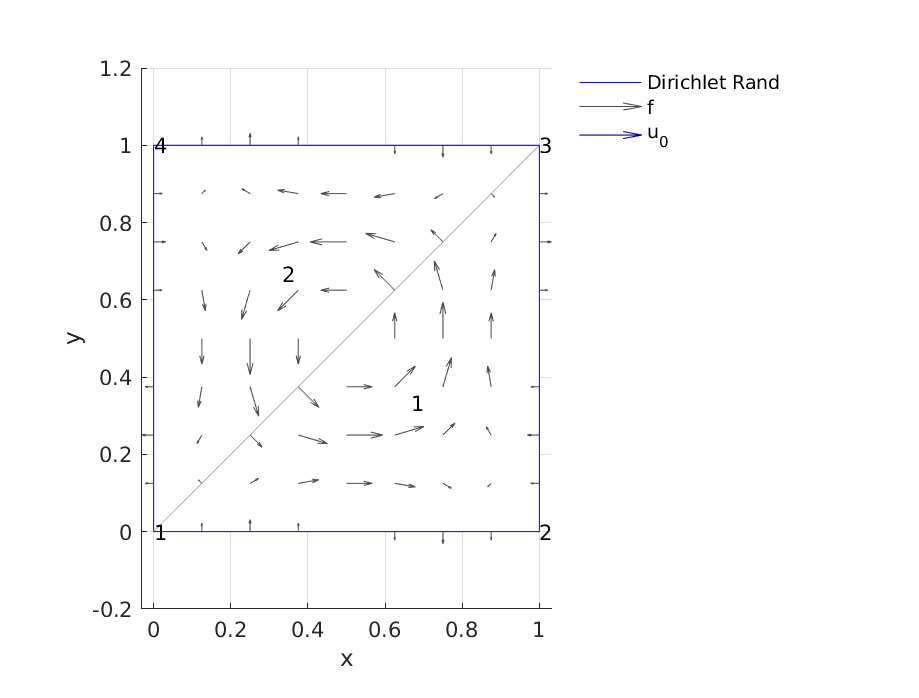
\includegraphics[width=\textwidth]{./Plots/SquareBenchmarkInitial1}
	    \caption{Anfangskonfiguration}
	\end{figure}
\end{frame}

\begin{frame}
	\begin{figure}[h]
	    \centering
	    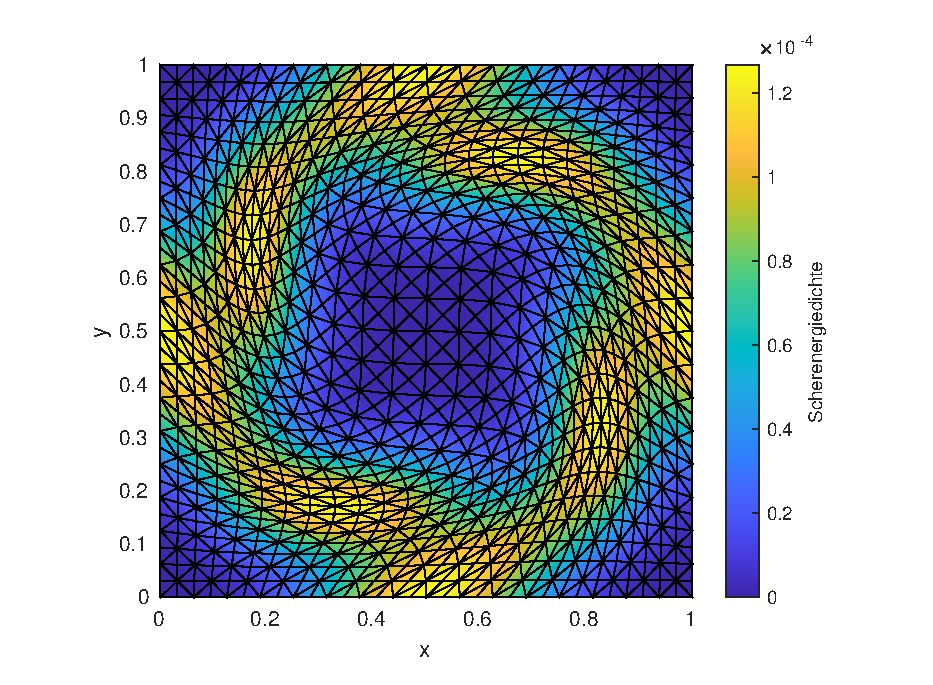
\includegraphics[width=\textwidth]{./Plots/SquareBenchmarkDeform2}
	    \caption{Mögliche Deformation des Gebiets}
	\end{figure}
\end{frame}

\begin{frame}
	\begin{figure}[h]
	    \centering
	    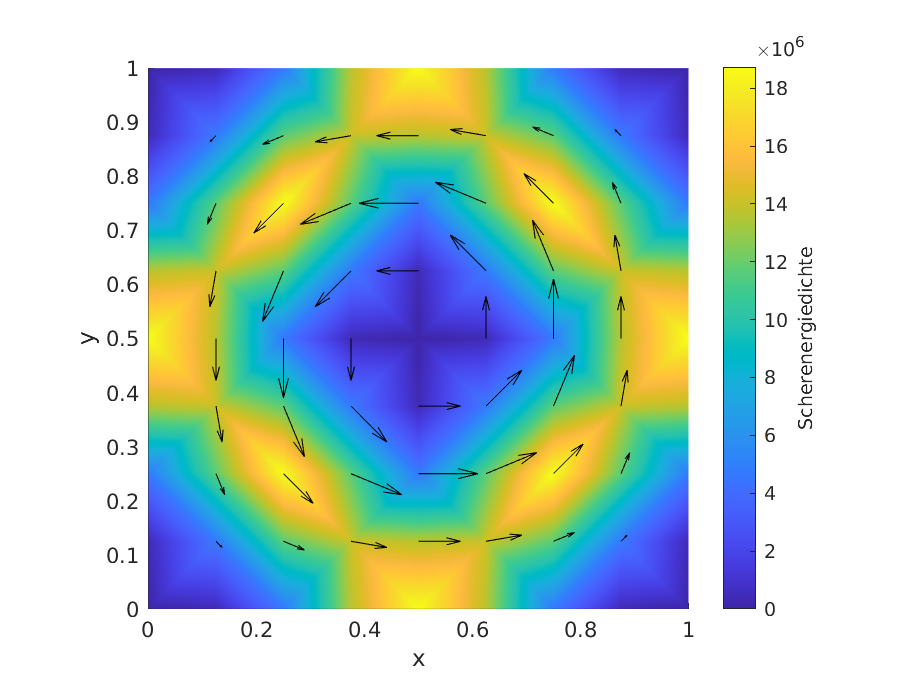
\includegraphics[width=\textwidth]{./Plots/SquareBenchmarkSoln1}
	    \caption{Lösung auf dem Gebiet}
	\end{figure}
\end{frame}

\begin{frame}
	\begin{figure}[h]
	    \centering
	    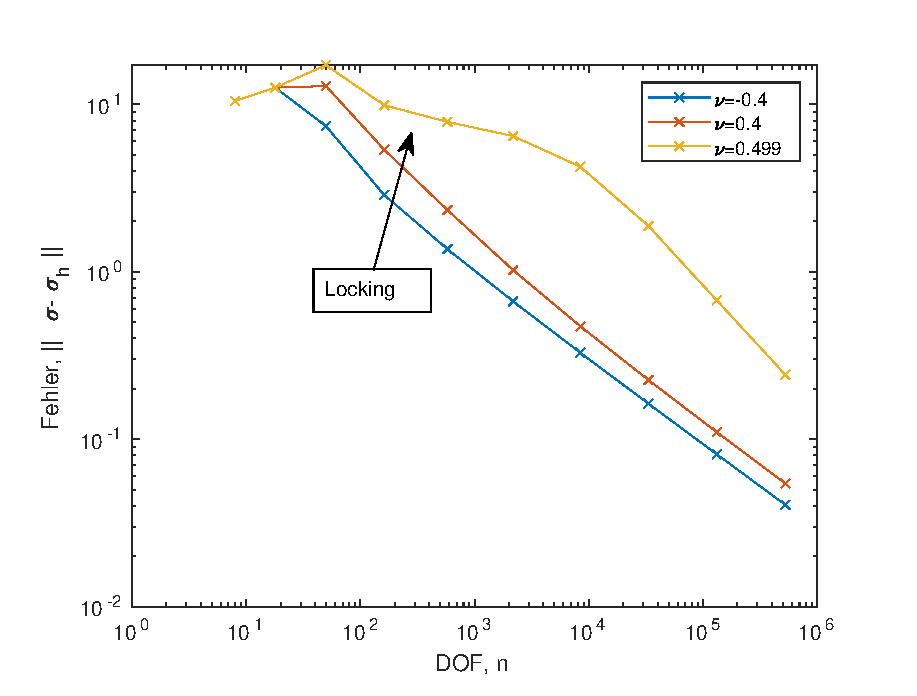
\includegraphics[width=\textwidth]{./Plots/SquareBenchmarkError1}
	    \caption{Fehler}
	\end{figure}
\end{frame}

\begin{frame}
	\begin{figure}[h]
	    \centering
	    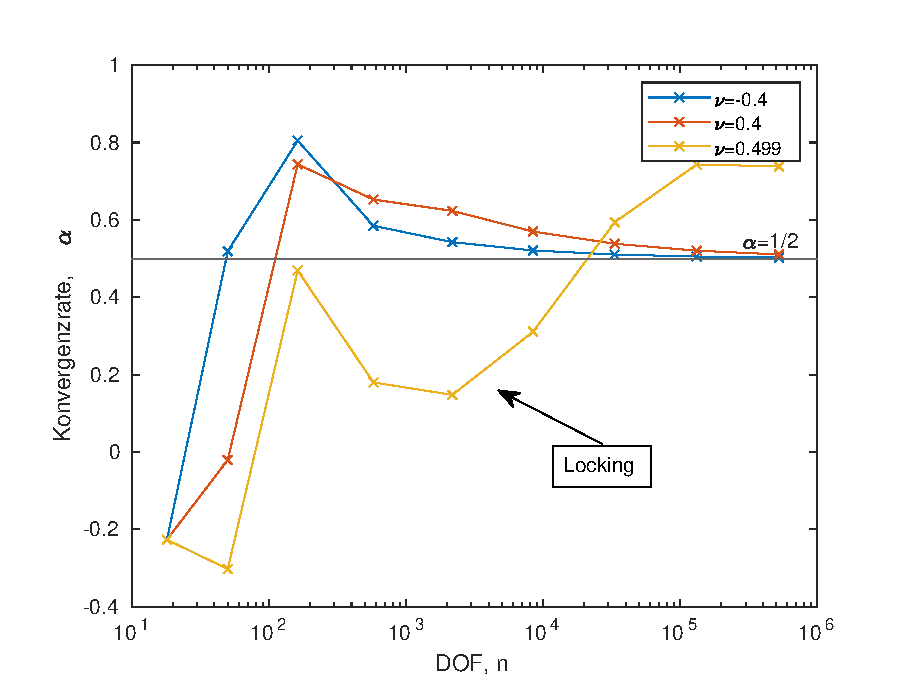
\includegraphics[width=\textwidth]{./Plots/SquareBenchmarkConvergenceRate1}
	    \caption{Konvergenzrate}
	\end{figure}
\end{frame}

\begin{frame}
	\begin{figure}[h]
	    \centering
	    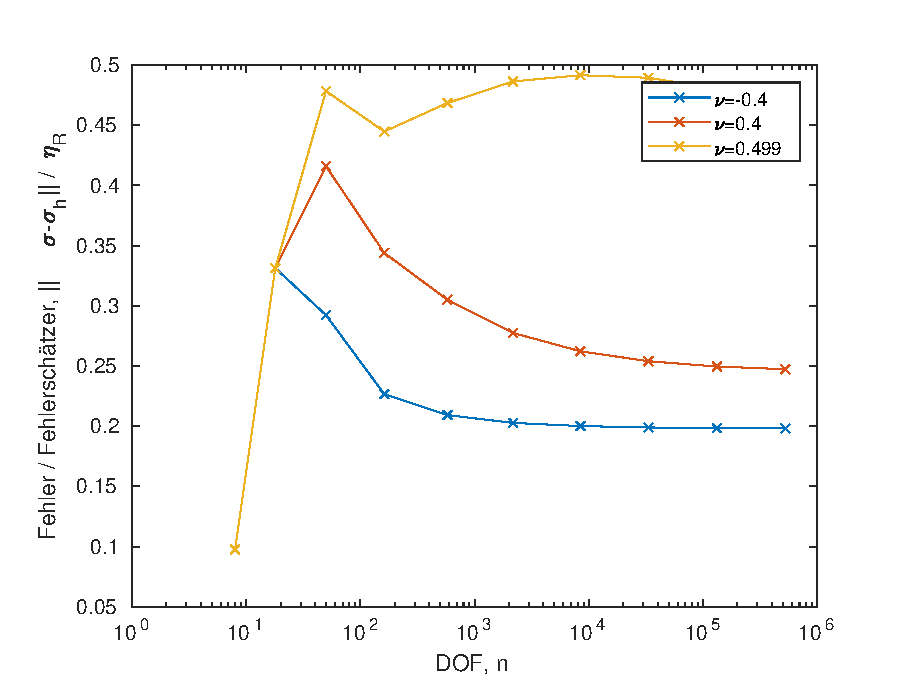
\includegraphics[width=\textwidth]{./Plots/SquareBenchmarkConsistency1}
	    \caption{Zuverlässigkeit}
	\end{figure}
\end{frame}

\begin{frame}
	\begin{figure}[h]
	    \centering
	    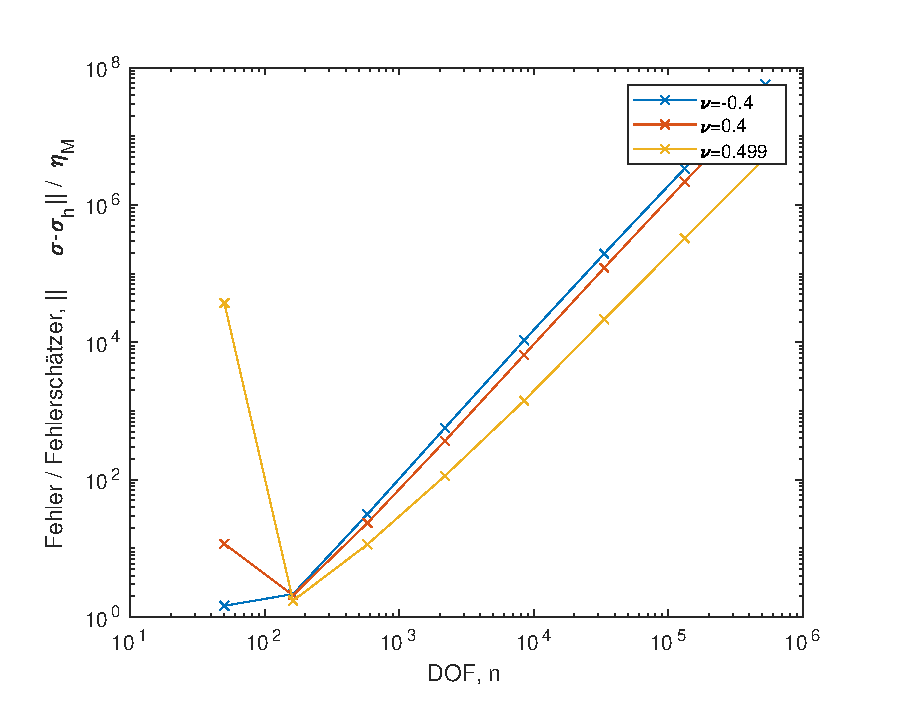
\includegraphics[width=\textwidth]{./Plots/SquareBenchmarkInconsistency1}
	    \caption{Auf eine andere Art zuverlässig?}
	\end{figure}
\end{frame}

\subsection*{Benchmark: L-förmiges Gebiet}
\begin{frame}
	Das Folgende Benchmark ist aus \cite{Car-2011,Alb-2002}
	\begin{block}{Benchmark: L-förmiges Gebiet}
	Wir verwenden ein L-förmiges gebiet mit reinem Dirichlet-Rand und Parameten $E=10^6$, $\nu=0.3$ und $\delta=0.7$. $u$ ist
	In Polarkoordinaten gegeben durch
	\begin{align*}
		u_r(r,\phi) &= \frac{r^\alpha}{2\mu}\big(-(\alpha+1)\cos\left((\alpha+1)\phi\right) \\
		&\qquad\qquad+(C_2-\alpha-1)C_1\cos\left((\alpha-1)\phi\right)\big) \\
		u_r(r,\phi) &= \frac{r^\alpha}{2\mu}\big((\alpha+1)\sin\left((\alpha+1)\phi\right) \\
		&\qquad\qquad+(C_2+\alpha-1)C_1\sin\left((\alpha-1)\phi\right)\big)
	\end{align*}
	mit speziellen Konstanten $C_1$, $C_2$ und $\alpha$. $f$ ist gegeben durch
	$f = 0$
	\end{block}
\end{frame}


\begin{frame}
	\begin{figure}[h]
	    \centering
	    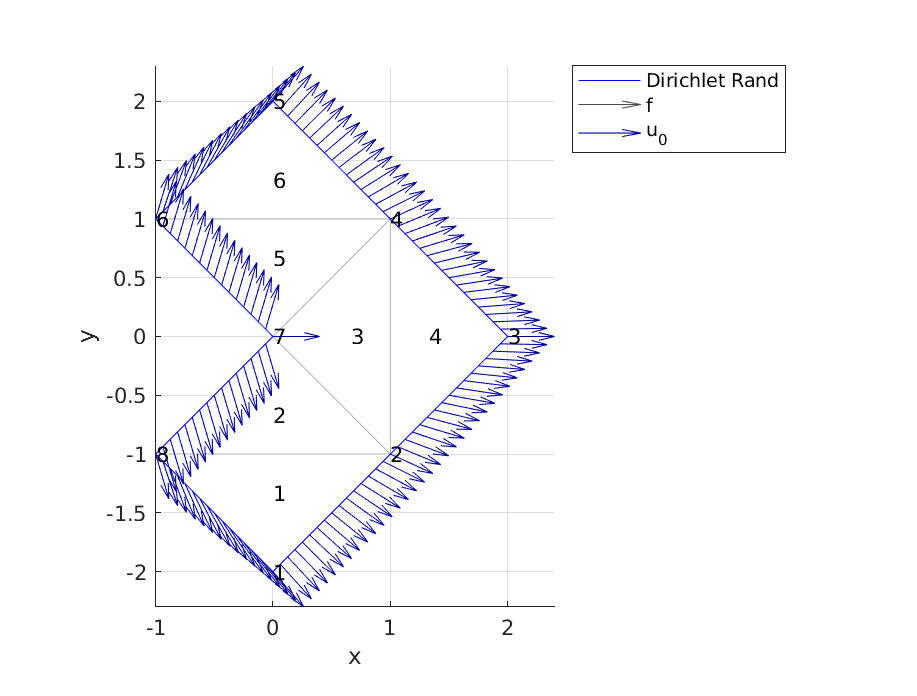
\includegraphics[width=\textwidth]{./Plots/LShapeBenchmarkInitial2}
	    \caption{Anfangskonfiguration}
	\end{figure}
\end{frame}

\begin{frame}
	\begin{figure}[h]
	    \centering
	    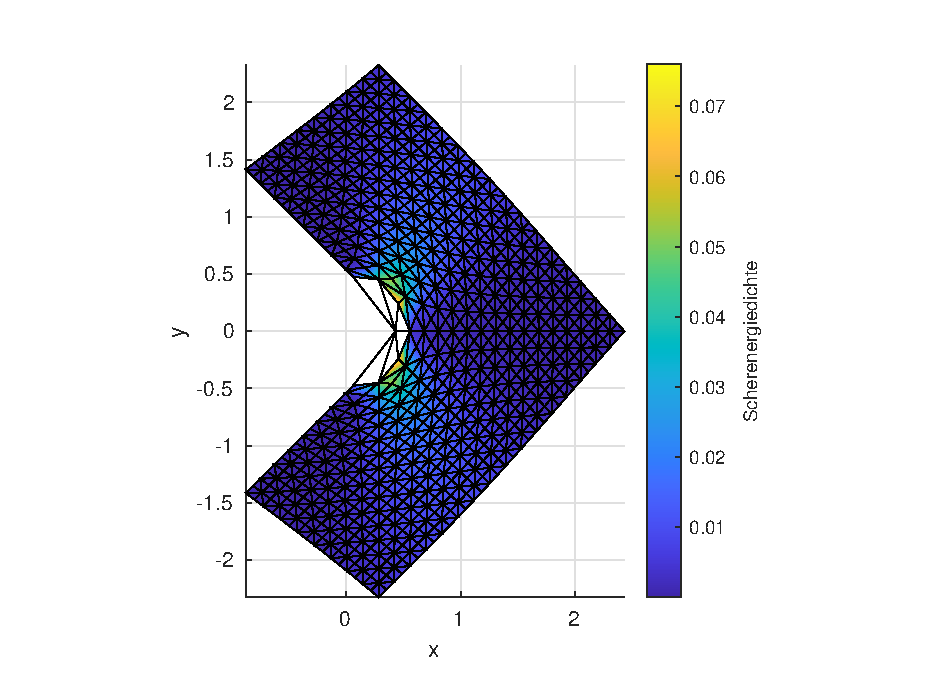
\includegraphics[width=\textwidth]{./Plots/LShapeBenchmarkDeform2}
	    \caption{Mögliche Deformation des Gebiets}
	\end{figure}
\end{frame}

\begin{frame}
	\begin{figure}[h]
	    \centering
	    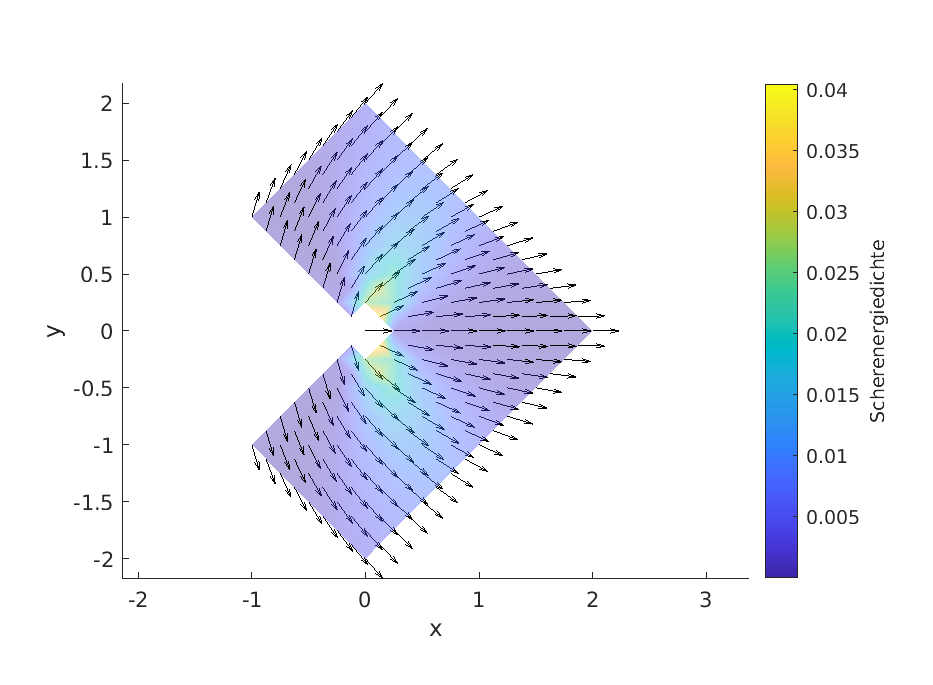
\includegraphics[width=\textwidth]{./Plots/LShapeBenchmarkSoln2}
	    \caption{Lösung auf dem Gebiet}
	\end{figure}
\end{frame}

\begin{frame}
	\begin{figure}[h]
	    \centering
	    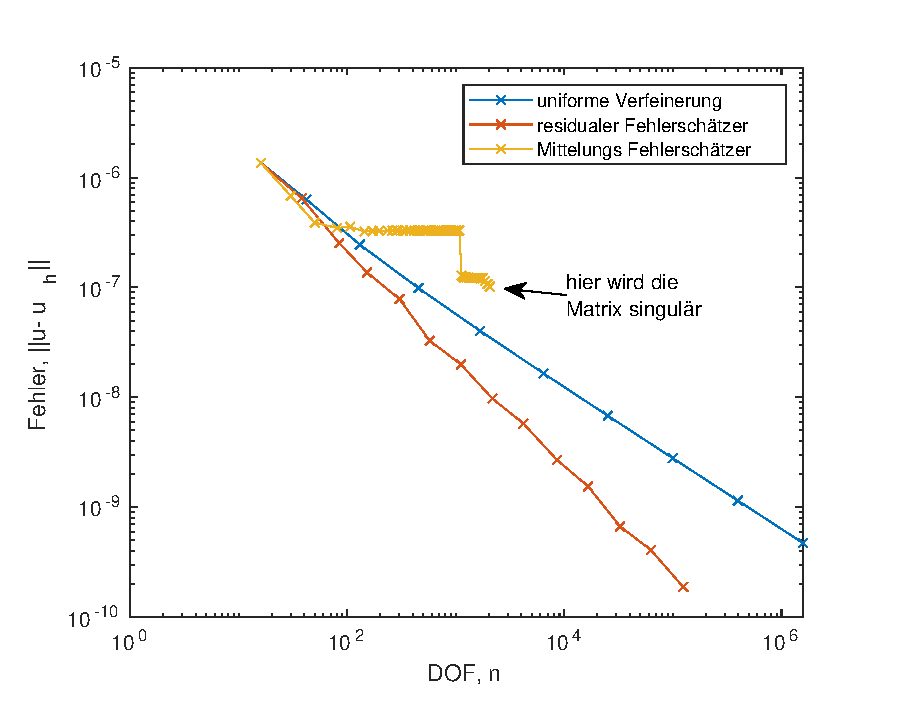
\includegraphics[width=\textwidth]{./Plots/LShapeBenchmarkError1}
	    \caption{Fehler}
	\end{figure}
\end{frame}

\begin{frame}
	\begin{figure}[h]
	    \centering
	    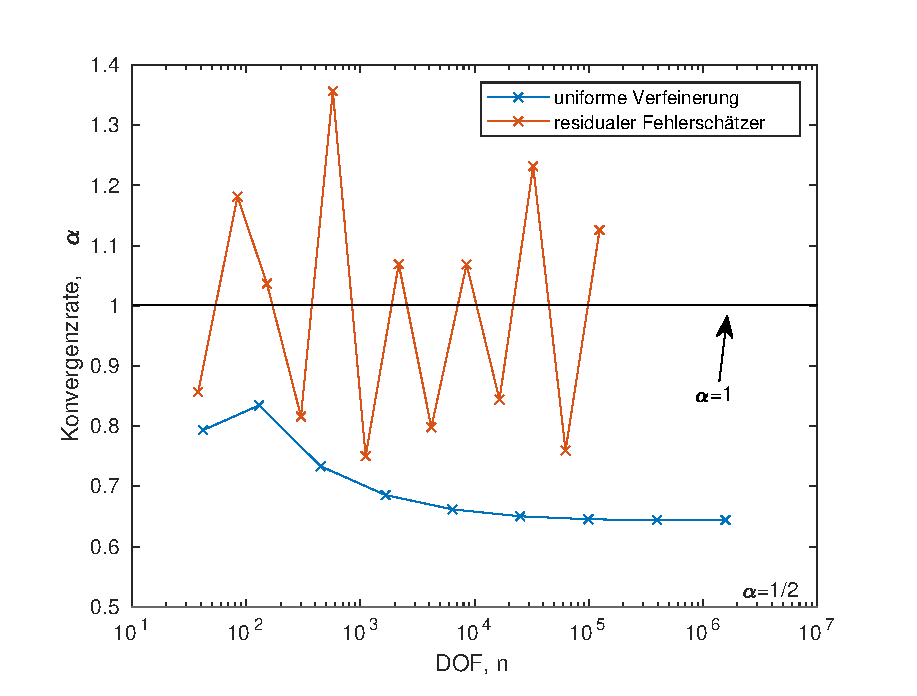
\includegraphics[width=\textwidth]{./Plots/LShapeBenchmarkConvergence1}
	    \caption{Konvergenzrate}
	\end{figure}
\end{frame}

\begin{frame}
	\begin{figure}
		\centering
		\begin{subfigure}[b]{0.45\textwidth}
	    \centering
	    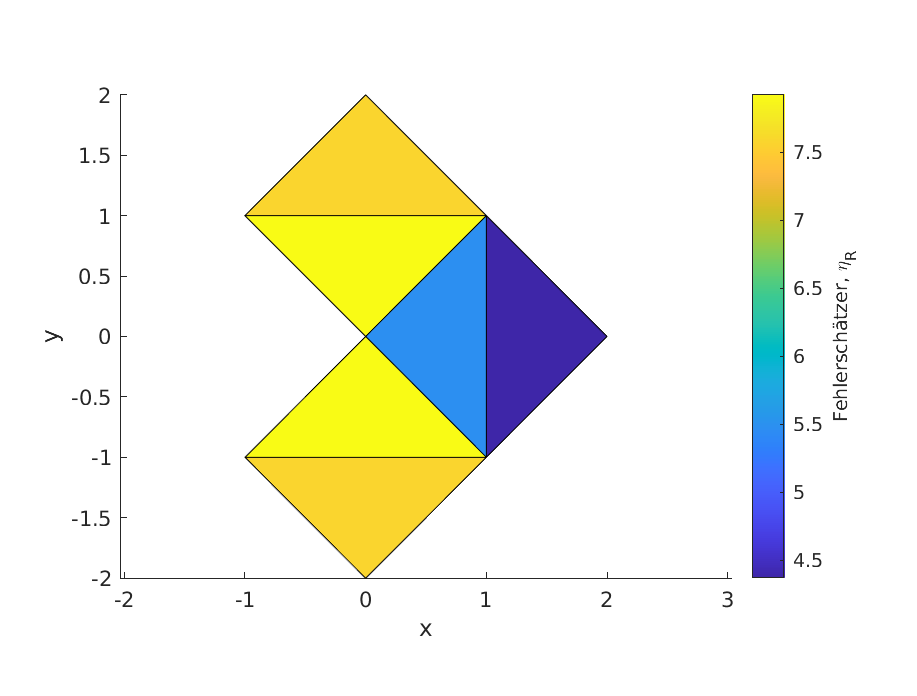
\includegraphics[width=\textwidth]{./Plots/LShapeBenchmarkUniformLocalEstim1}
	    \caption{Fehlerschätzer}
	    \end{subfigure}
	    \begin{subfigure}[b]{0.45\textwidth}
	    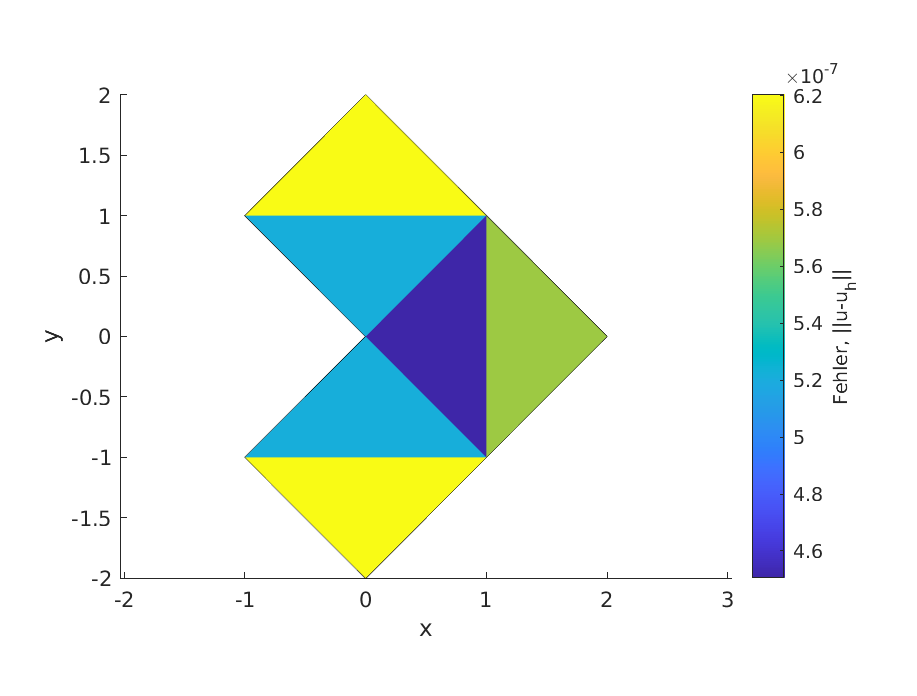
\includegraphics[width=\textwidth]{./Plots/LShapeBenchmarkUniformLocalError1}
	    \caption{Fehler}
	    \end{subfigure}
	    \caption{uniforme Triangulierung bei $DOF=16$}
	\end{figure}
\end{frame}

\begin{frame}
	\begin{figure}
		\centering
		\begin{subfigure}[b]{0.45\textwidth}
	    \centering
	    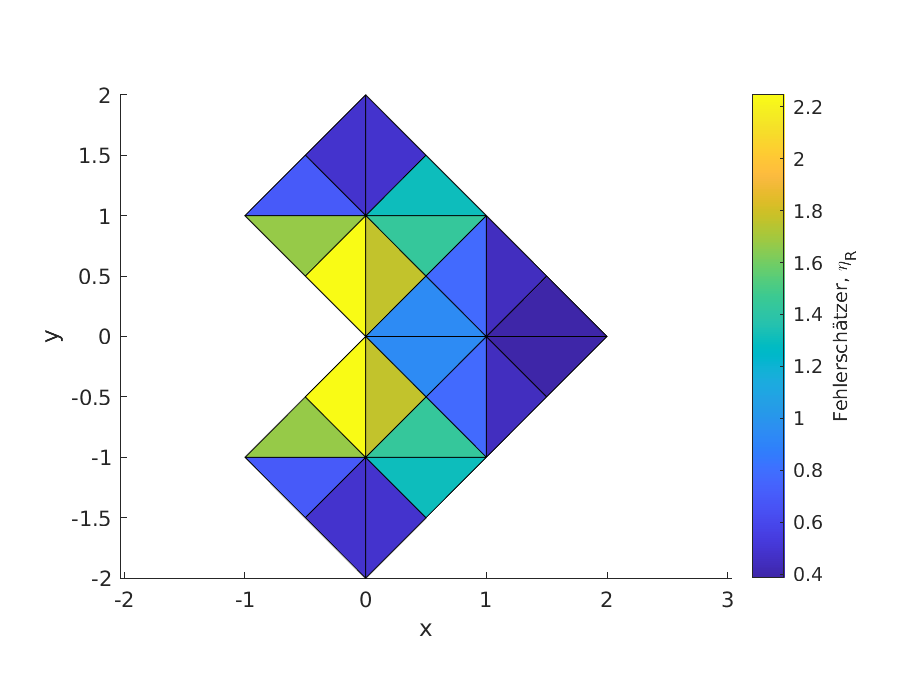
\includegraphics[width=\textwidth]{./Plots/LShapeBenchmarkUniformLocalEstim2}
	    \caption{Fehlerschätzer}
	    \end{subfigure}
	    \begin{subfigure}[b]{0.45\textwidth}
	    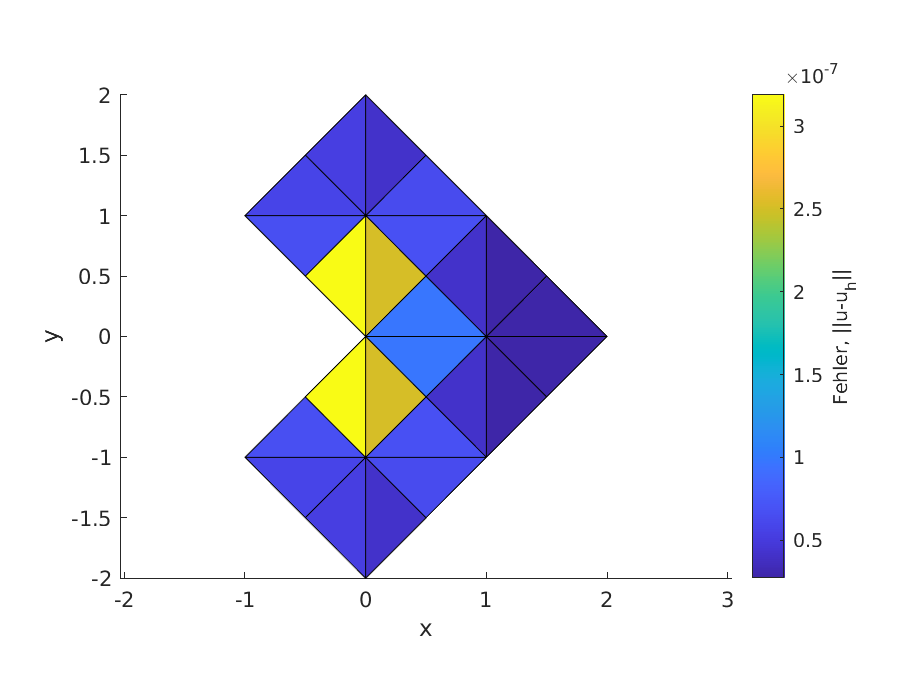
\includegraphics[width=\textwidth]{./Plots/LShapeBenchmarkUniformLocalError2}
	    \caption{Fehler}
	    \end{subfigure}
	    \caption{uniforme Triangulierung bei $DOF=42$}
	\end{figure}
\end{frame}

\begin{frame}
	\begin{figure}
		\centering
		\begin{subfigure}[b]{0.45\textwidth}
	    \centering
	    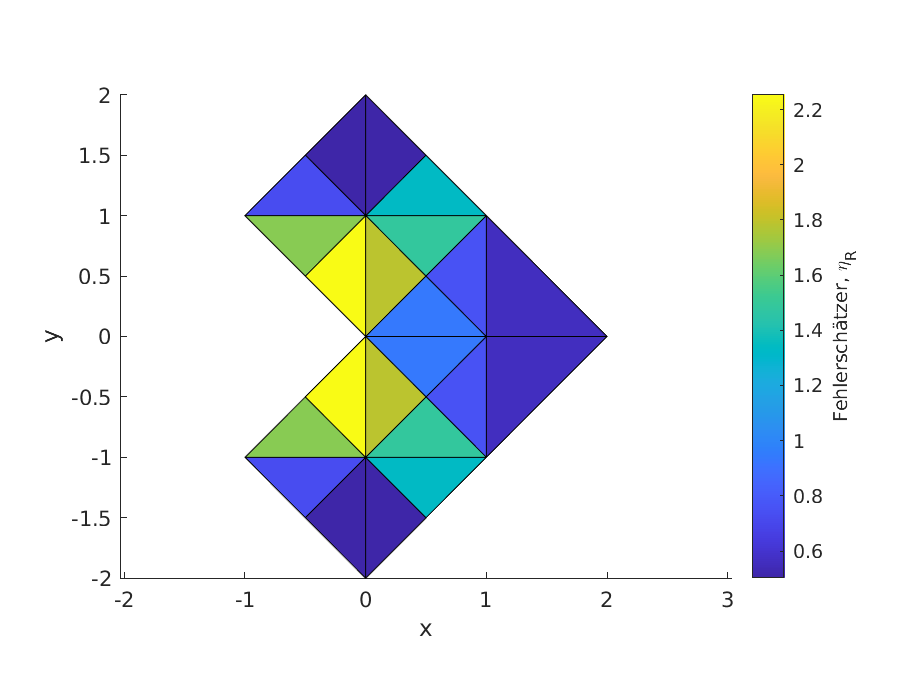
\includegraphics[width=\textwidth]{./Plots/LShapeBenchmarkResidualLocalEstim2}
	    \caption{Fehlerschätzer}
	    \end{subfigure}
	    \begin{subfigure}[b]{0.45\textwidth}
	    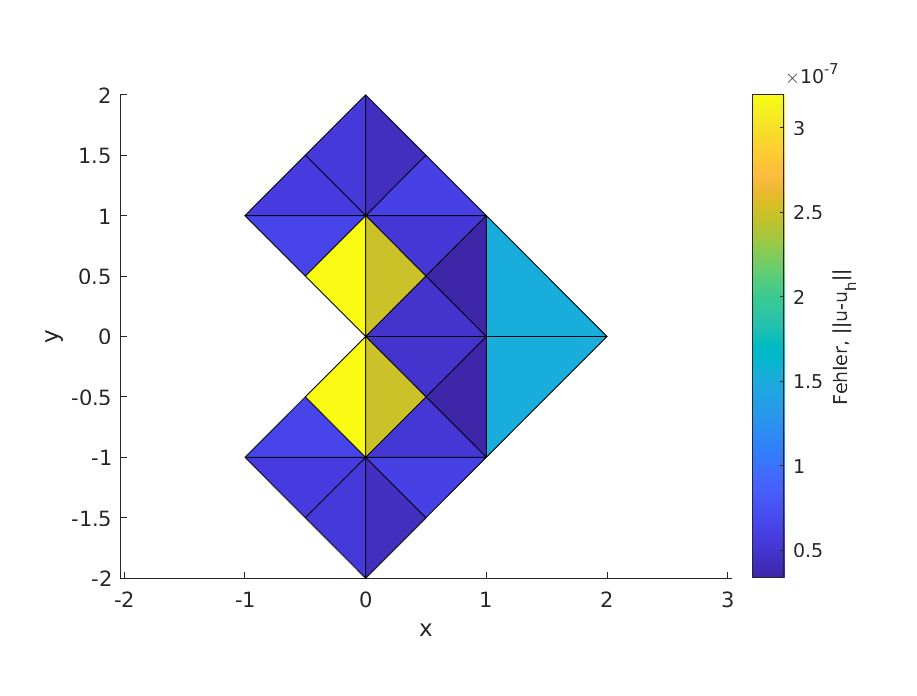
\includegraphics[width=\textwidth]{./Plots/LShapeBenchmarkResidualLocalError2}
	    \caption{Fehler}
	    \end{subfigure}
	    \caption{Triangulierung für den residualen Schätzer bei $DOF=38$}
	\end{figure}
\end{frame}
\begin{frame}
	\begin{figure}
		\centering
		\begin{subfigure}[b]{0.45\textwidth}
	    \centering
	    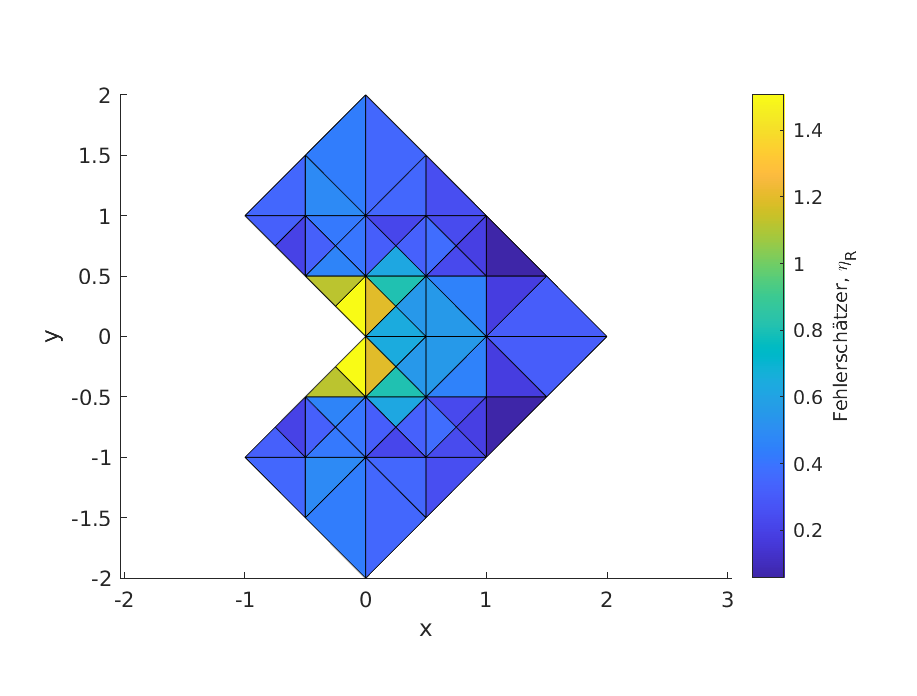
\includegraphics[width=\textwidth]{./Plots/LShapeBenchmarkResidualLocalEstim3}
	    \caption{Fehlerschätzer}
	    \end{subfigure}
	    \begin{subfigure}[b]{0.45\textwidth}
	    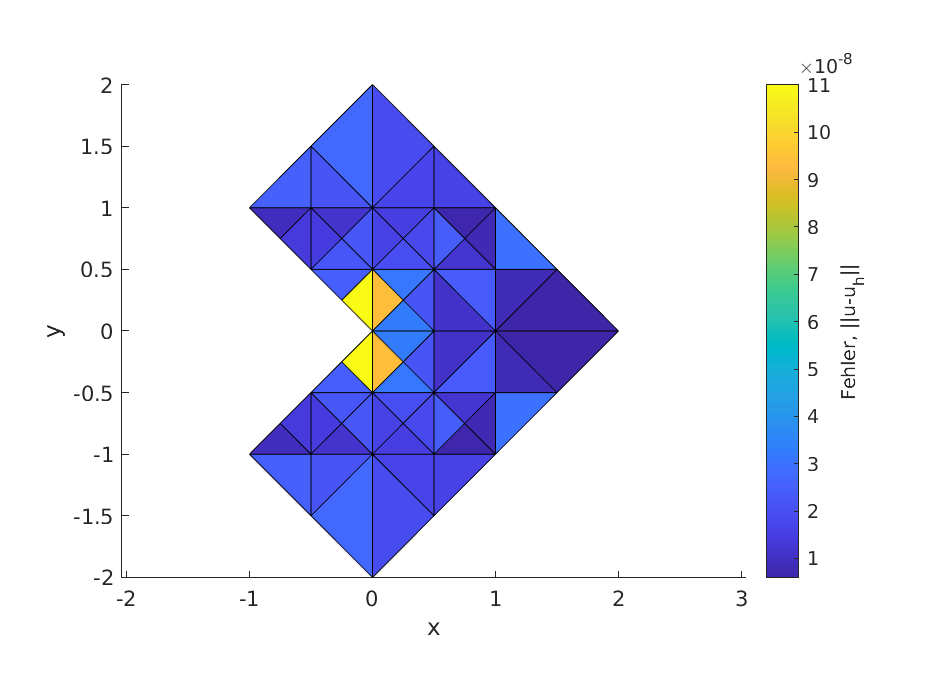
\includegraphics[width=\textwidth]{./Plots/LShapeBenchmarkResidualLocalError3}
	    \caption{Fehler}
	    \end{subfigure}
	    \caption{Triangulierung für den residualen Schätzer bei $DOF=84$}
	\end{figure}
\end{frame}


\begin{frame}
	\begin{figure}
		\centering
		\begin{subfigure}[b]{0.45\textwidth}
	    \centering
	    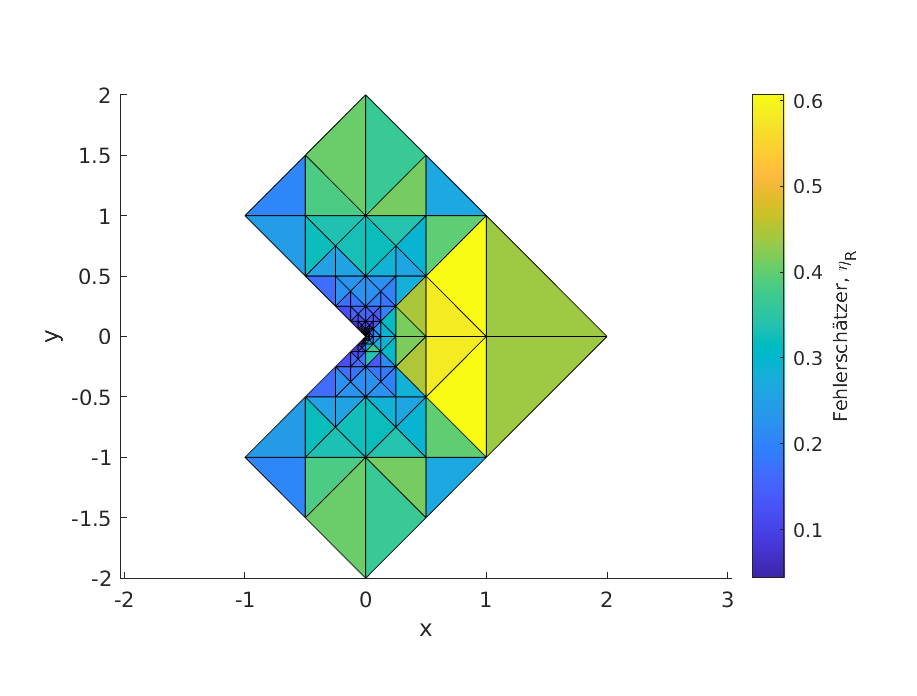
\includegraphics[width=\textwidth]{./Plots/LShapeBenchmarkAverageLocalEstim1}
	    \caption{Fehlerschätzer}
	    \end{subfigure}
	    \begin{subfigure}[b]{0.45\textwidth}
	    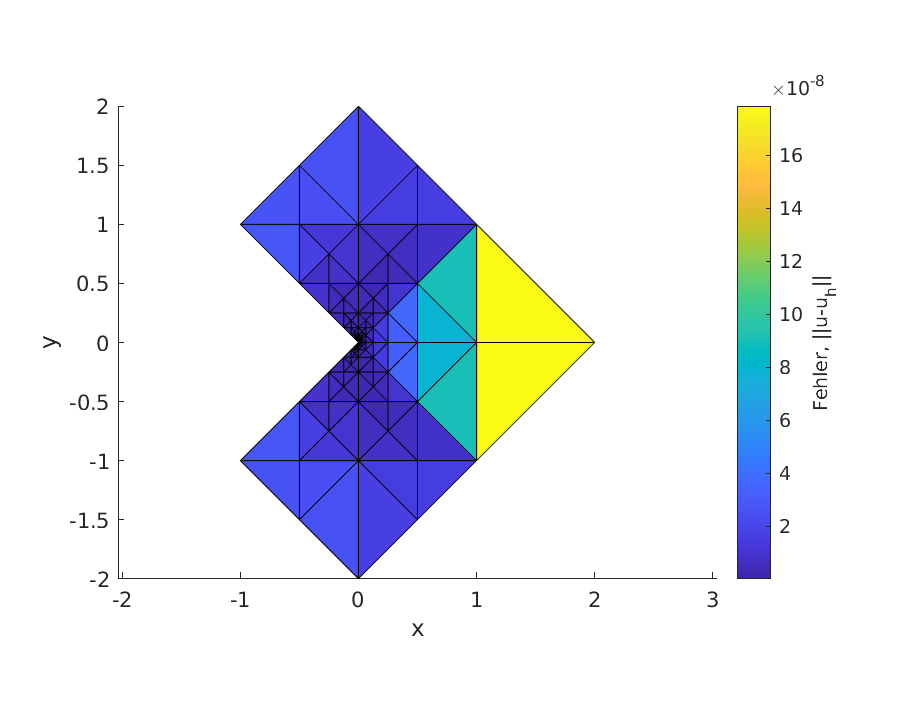
\includegraphics[width=\textwidth]{./Plots/LShapeBenchmarkAverageLocalError1}
	    \caption{Fehler}
	    \end{subfigure}
	    \caption{Triangulation für den Mittelungs Fehlerschätzer bei $DOF=196$}
	\end{figure}
\end{frame}
\begin{frame}
	\begin{figure}
		\centering
		\begin{subfigure}[b]{0.45\textwidth}
	    \centering
	    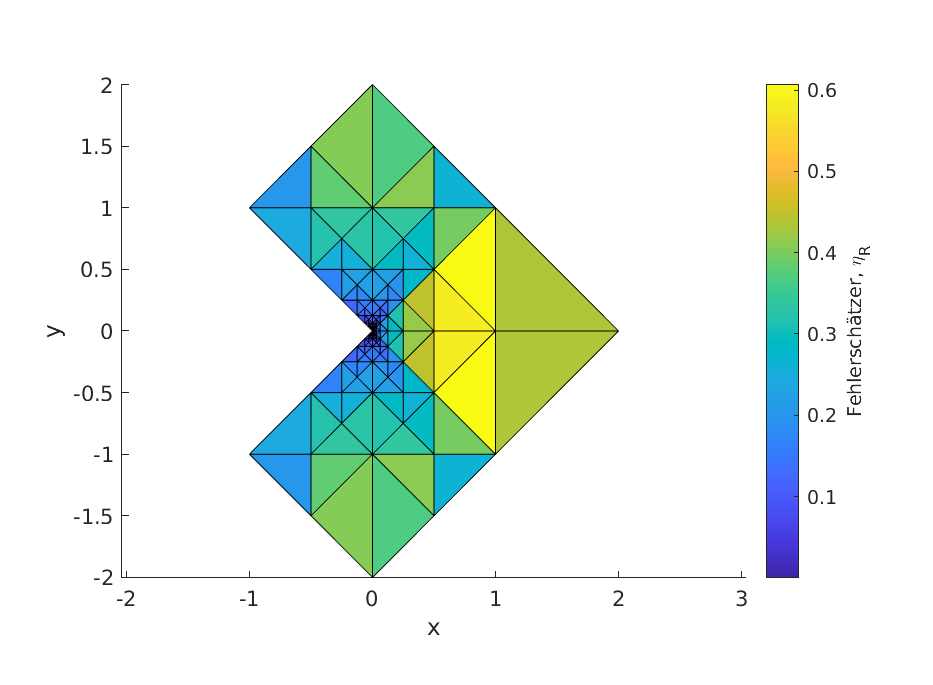
\includegraphics[width=\textwidth]{./Plots/LShapeBenchmarkAverageLocalEstim2}
	    \caption{Fehlerschätzer}
	    \end{subfigure}
	    \begin{subfigure}[b]{0.45\textwidth}
	    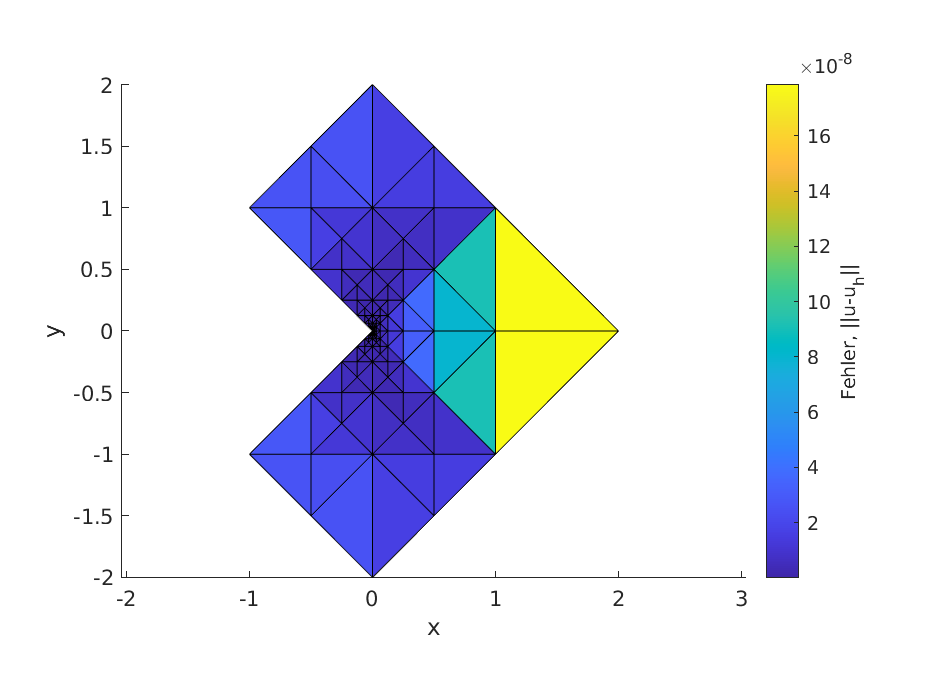
\includegraphics[width=\textwidth]{./Plots/LShapeBenchmarkAverageLocalError2}
	    \caption{Fehler}
	    \end{subfigure}
	    \caption{Triangulation für den Mittelungs Fehlerschätzer bei $DOF=1018$}
	\end{figure}
\end{frame}


\begin{frame}
	\begin{figure}
		\centering
		\begin{subfigure}[b]{0.45\textwidth}
	    \centering
	    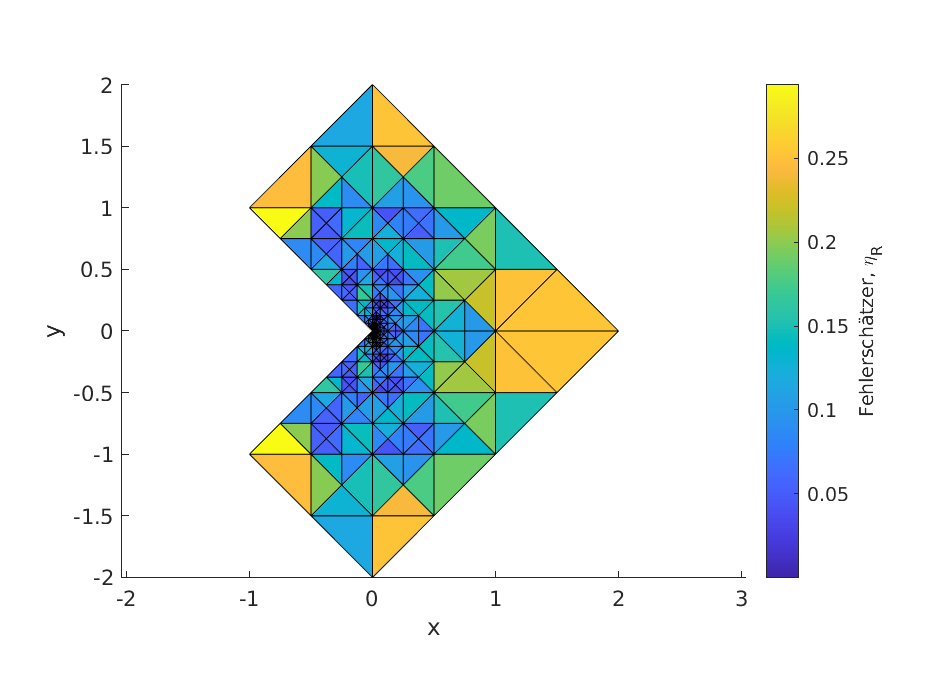
\includegraphics[width=\textwidth]{./Plots/LShapeBenchmarkAverageLocalEstim3}
	    \caption{Fehlerschätzer}
	    \end{subfigure}
	    \begin{subfigure}[b]{0.45\textwidth}
	    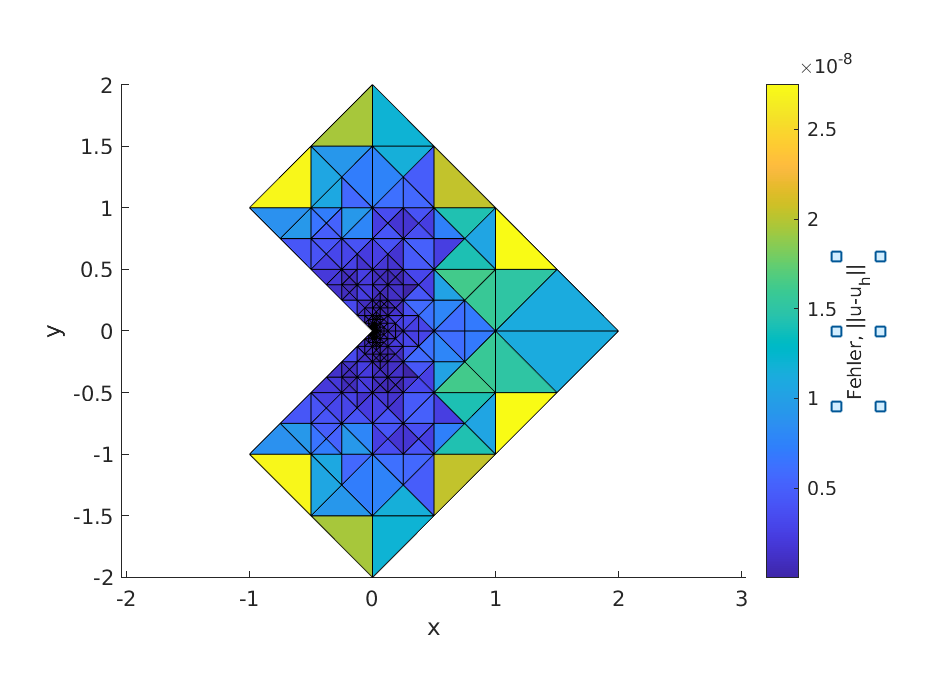
\includegraphics[width=\textwidth]{./Plots/LShapeBenchmarkAverageLocalError3}
	    \caption{Fehler}
	    \end{subfigure}
	    \caption{Triangulation für den Mittelungs Fehlerschätzer bei $DOF=1946$}
	\end{figure}
\end{frame}

\section{Zusammenfassung}
\begin{frame}[allowframebreaks]
	\frametitle{Zusammenfassung}
	
	Formulierungen des kontinuierlichen Problems: Finde $u\in V$, so dass
	\begin{itemize}
		\item
		Kräftegleichgewicht
		\begin{align*}
			\int_\omega f\dif x+\int_{\partial\omega}\sigma n\dif s&=0 &&\text{für alle }\omega\subseteq\Omega \\
			\sigma n&= g &&\text{auf }\Gamma_N \\
			Mu &= w &&\text{auf }\Gamma
		\end{align*}
		\item
		Differenzielles Problem
		\begin{align*}
			\qquad\qquad-\diver\sigma &= f &&\text{auf }\Omega\qquad\qquad\\
			\sigma n &= g &&\text{auf }\Gamma_N \\
			Mu &= w &&\text{auf }\Gamma
		\end{align*}
		\item
		Variationelles Problem (virtuelle Arbeit)
		\begin{align*}
			a(u,v)&= \ell(v) \qquad &&\text{für alle }v\in V^0\qquad\\
			Mu &= w &&\text{auf }\Gamma
		\end{align*}
		\item
		Optimierungsproblem (Energiefunktional)
		\begin{equation*}
			\begin{aligned}
				u\text{ minimiert }&&  &W=\frac{1}{2}a(\cdot,\cdot)-\ell \\
			\text{unter der Nebenbedingung }&&  &Mu\big\vert_\Gamma = w
			\end{aligned}
		\end{equation*}
	\end{itemize}
	Formulierungen des diskreten Problems: Finde $u_h\in V_h$, so dass
	\begin{itemize}
		\item
		Optimierungsproblem
		\begin{align*}
			\hu\text{ minimiert }&& \hW(\hv)&\coloneqq \frac{1}{2}\hv^\top A\hv-\hl^\top\hv \\
			\text{unter der Nebenbedingung }&& B\hu &= \hw
		\end{align*}
		\item
		LGS mit Lagrange-Multiplikatoren
		\begin{align*}
			\begin{bmatrix}
				A & B^\top \\
				B & 0
			\end{bmatrix}
			\vect{\hu \\ \hp}
			= \vect{\hl \\ \hw}
		\end{align*}
	\end{itemize}
	
	\begin{itemize}
		\item
		Man zeigt:
		
		
		Kornsche Ungleichung ohne Randbedinungen auf dem Ganzraum $\xrightarrow{\text{Erweiterungsoperator}}$ Kornsche Ungleichung ohne Randbedingungen $\xrightarrow{\text{Starrk"orperbewegungen}}$ Kornsche Ungleichung mit Randbedingungen $\rightarrow$ Positivdefinitheit von $a$
		\item
		Existenz und Eindeutigkeit
		\begin{itemize}
			\item 
			kontinuierliches Problem: Lax-Milgram-Lemma
			\item
			diskretes Problem: Resultate aus der quadratischen Optimierung
		\end{itemize}
		\item
		Der residuale Fehlerschätzer ist verlässlich (reliable) und effizient. Dies sieht man auch in numerischen Experimenten.
		\item
		Der residuale Fehlerschätzer wird verwendet, um das Gitter adaptiv zu verfeinern. Dies verbessert bei manchen Problemen die Konvergenz.
	\end{itemize}
\end{frame}

\begin{frame}
	\begin{center}
		\Large{{Danke für die Aufmerksamkeit.}}
	\end{center}
\end{frame}

\begin{frame}
	\begin{center}
		\Large{{Fragen?}}
	\end{center}
\end{frame}


\section{Quellen}
\begin{frame}[allowframebreaks]
	\frametitle{Quellen}
	\setbeamertemplate{bibliography item}[text]
	\begin{thebibliography}{0000}
		
		\bibitem{Alb-2002}
		Alberty, J., C. Carstensen, S. A. Funken, and R. Klose.
		"Matlab Implementation of the Finite Element Method in Elasticity."
		{\em Computing 69}, no. 3 (2002): 239-263. 
		
		\bibitem{Alt-2016}
		Alt, Hans Wilhelm.
		{\em Linear Functional Analysis: An Application-Oriented Introduction.}
		London: Springer London, 2016. 
		
		\bibitem{Ban-2003}
		Bangerth, Wolfgang, and Rolf Rannacher.
		{\em Adaptive Finite Element Methods for Differential Equations.}
		Basel [u.a.]: Birkhäuser, 2003. S.130f.
		
		\bibitem{Bra-2007}
		Braess, Dietrich.
		{\em Finite Elemente: Theorie, Schnelle Löser Und Anwendungen in Der Elastizitätstheorie.}
		4., überarb. und erw. Aufl.
		Berlin [u.a.]: Springer, 2007.
		
		\bibitem{Car-2011}
		Carstensen, C., M. Eigel, and J. Gedicke.
		''Computational Competition of Symmetric Mixed FEM in Linear Elasticity.''
		{\em Computer Methods in Applied Mechanics and Engineering 200}.41 (2011): 2903-2915.
		
		\bibitem{Cia-1988}
		Ciarlet, Philippe G.
		{\em Studies in Mathematics and Its Applications. Mathematical Elasticity. 1, Three-dimensional Elasticity.}
		Amsterdam [u.a.]: North-Holland, 1988.
		
		\bibitem{Cia-1997}
		Ciarlet, Philippe G.
		{\em Studies in Mathematics and Its Applications. Mathematical Elasticity. 2, Theory of Plates.}
		Amsterdam [u.a.]: North-Holland, 1997. 
		
		\bibitem{Con-2021}
		Conti, S.
		''Einführung in die Funktionanalysis''.
		Vorlesungsnotizen. Universität Bonn, Wintersemester 2021/2022.
		
		\bibitem{Duv-1976}
		Lions, Jacques Louis, and Georges Duvaut.
		{\em Inequalities in Mechanics and Physics.}
		Berlin, Heidelberg: Springer, 1976. 
		
		\bibitem{Gei-2002}
		Geiger, Carl.
		{\em Theorie Und Numerik Restringierter Optimierungsaufgaben.}
		1st ed. 2002. Berlin, Heidelberg: Springer Berlin Heidelberg, 2002.
		
		\bibitem{Ged-2021a}
		Gedicke, J.
		''Einführung in die Numerische Mathematik''.
		Vorlesungsnotizen. Universität Bonn, Sommersemester 2021.
		
		\bibitem{Ged-2021b}
		Gedicke, J.
		''Wissenschaftliches Rechnen I''.
		Vorlesungsnotizen. Universität Bonn, Wintersemester 2021/2022.
		
		\bibitem{Kik-1988}
		Kikuchi, Noboru, and John Tinsley Oden.
		{\em Contact Problems in Elasticity: A Study of Variational Inequalities and Finite Element Methods.}
		Philadelphia: SIAM, 1988. 
		
		\bibitem{Lif-1959}
		Lifshitz, Evgenii Mikhailovich, and Lev Davidovich Landau.
		{\em Course of Theoretical Physics.}
		Pergamon, 1959.
		
		\bibitem{Nit-1981}
		Nitsche, J. A.
		{\em On Korn's second inequality.}
		RAIRO Anal. Numér.  15  (1981),  no. 3, 237--248.

	\end{thebibliography}
\end{frame}
%		
%		\bibitem{Nei-2004}
%		Neittaanmäki, Pekka, and Sergey R. Repin.
%		{\em Reliable Methods for Computer Simulation: Error Control and Posteriori Estimates}.
%		Oxford: Elsevier Science \& Technology, 2004.


\frame[plain]

\end{document}
